% Options for packages loaded elsewhere
\PassOptionsToPackage{unicode}{hyperref}
\PassOptionsToPackage{hyphens}{url}
%
\documentclass[
]{book}
\title{A Minimal Book Example}
\author{John Doe}
\date{2022-06-08}

\usepackage{amsmath,amssymb}
\usepackage{lmodern}
\usepackage{iftex}
\ifPDFTeX
  \usepackage[T1]{fontenc}
  \usepackage[utf8]{inputenc}
  \usepackage{textcomp} % provide euro and other symbols
\else % if luatex or xetex
  \usepackage{unicode-math}
  \defaultfontfeatures{Scale=MatchLowercase}
  \defaultfontfeatures[\rmfamily]{Ligatures=TeX,Scale=1}
\fi
% Use upquote if available, for straight quotes in verbatim environments
\IfFileExists{upquote.sty}{\usepackage{upquote}}{}
\IfFileExists{microtype.sty}{% use microtype if available
  \usepackage[]{microtype}
  \UseMicrotypeSet[protrusion]{basicmath} % disable protrusion for tt fonts
}{}
\makeatletter
\@ifundefined{KOMAClassName}{% if non-KOMA class
  \IfFileExists{parskip.sty}{%
    \usepackage{parskip}
  }{% else
    \setlength{\parindent}{0pt}
    \setlength{\parskip}{6pt plus 2pt minus 1pt}}
}{% if KOMA class
  \KOMAoptions{parskip=half}}
\makeatother
\usepackage{xcolor}
\IfFileExists{xurl.sty}{\usepackage{xurl}}{} % add URL line breaks if available
\IfFileExists{bookmark.sty}{\usepackage{bookmark}}{\usepackage{hyperref}}
\hypersetup{
  pdftitle={A Minimal Book Example},
  pdfauthor={John Doe},
  hidelinks,
  pdfcreator={LaTeX via pandoc}}
\urlstyle{same} % disable monospaced font for URLs
\usepackage{color}
\usepackage{fancyvrb}
\newcommand{\VerbBar}{|}
\newcommand{\VERB}{\Verb[commandchars=\\\{\}]}
\DefineVerbatimEnvironment{Highlighting}{Verbatim}{commandchars=\\\{\}}
% Add ',fontsize=\small' for more characters per line
\usepackage{framed}
\definecolor{shadecolor}{RGB}{248,248,248}
\newenvironment{Shaded}{\begin{snugshade}}{\end{snugshade}}
\newcommand{\AlertTok}[1]{\textcolor[rgb]{0.94,0.16,0.16}{#1}}
\newcommand{\AnnotationTok}[1]{\textcolor[rgb]{0.56,0.35,0.01}{\textbf{\textit{#1}}}}
\newcommand{\AttributeTok}[1]{\textcolor[rgb]{0.77,0.63,0.00}{#1}}
\newcommand{\BaseNTok}[1]{\textcolor[rgb]{0.00,0.00,0.81}{#1}}
\newcommand{\BuiltInTok}[1]{#1}
\newcommand{\CharTok}[1]{\textcolor[rgb]{0.31,0.60,0.02}{#1}}
\newcommand{\CommentTok}[1]{\textcolor[rgb]{0.56,0.35,0.01}{\textit{#1}}}
\newcommand{\CommentVarTok}[1]{\textcolor[rgb]{0.56,0.35,0.01}{\textbf{\textit{#1}}}}
\newcommand{\ConstantTok}[1]{\textcolor[rgb]{0.00,0.00,0.00}{#1}}
\newcommand{\ControlFlowTok}[1]{\textcolor[rgb]{0.13,0.29,0.53}{\textbf{#1}}}
\newcommand{\DataTypeTok}[1]{\textcolor[rgb]{0.13,0.29,0.53}{#1}}
\newcommand{\DecValTok}[1]{\textcolor[rgb]{0.00,0.00,0.81}{#1}}
\newcommand{\DocumentationTok}[1]{\textcolor[rgb]{0.56,0.35,0.01}{\textbf{\textit{#1}}}}
\newcommand{\ErrorTok}[1]{\textcolor[rgb]{0.64,0.00,0.00}{\textbf{#1}}}
\newcommand{\ExtensionTok}[1]{#1}
\newcommand{\FloatTok}[1]{\textcolor[rgb]{0.00,0.00,0.81}{#1}}
\newcommand{\FunctionTok}[1]{\textcolor[rgb]{0.00,0.00,0.00}{#1}}
\newcommand{\ImportTok}[1]{#1}
\newcommand{\InformationTok}[1]{\textcolor[rgb]{0.56,0.35,0.01}{\textbf{\textit{#1}}}}
\newcommand{\KeywordTok}[1]{\textcolor[rgb]{0.13,0.29,0.53}{\textbf{#1}}}
\newcommand{\NormalTok}[1]{#1}
\newcommand{\OperatorTok}[1]{\textcolor[rgb]{0.81,0.36,0.00}{\textbf{#1}}}
\newcommand{\OtherTok}[1]{\textcolor[rgb]{0.56,0.35,0.01}{#1}}
\newcommand{\PreprocessorTok}[1]{\textcolor[rgb]{0.56,0.35,0.01}{\textit{#1}}}
\newcommand{\RegionMarkerTok}[1]{#1}
\newcommand{\SpecialCharTok}[1]{\textcolor[rgb]{0.00,0.00,0.00}{#1}}
\newcommand{\SpecialStringTok}[1]{\textcolor[rgb]{0.31,0.60,0.02}{#1}}
\newcommand{\StringTok}[1]{\textcolor[rgb]{0.31,0.60,0.02}{#1}}
\newcommand{\VariableTok}[1]{\textcolor[rgb]{0.00,0.00,0.00}{#1}}
\newcommand{\VerbatimStringTok}[1]{\textcolor[rgb]{0.31,0.60,0.02}{#1}}
\newcommand{\WarningTok}[1]{\textcolor[rgb]{0.56,0.35,0.01}{\textbf{\textit{#1}}}}
\usepackage{longtable,booktabs,array}
\usepackage{calc} % for calculating minipage widths
% Correct order of tables after \paragraph or \subparagraph
\usepackage{etoolbox}
\makeatletter
\patchcmd\longtable{\par}{\if@noskipsec\mbox{}\fi\par}{}{}
\makeatother
% Allow footnotes in longtable head/foot
\IfFileExists{footnotehyper.sty}{\usepackage{footnotehyper}}{\usepackage{footnote}}
\makesavenoteenv{longtable}
\usepackage{graphicx}
\makeatletter
\def\maxwidth{\ifdim\Gin@nat@width>\linewidth\linewidth\else\Gin@nat@width\fi}
\def\maxheight{\ifdim\Gin@nat@height>\textheight\textheight\else\Gin@nat@height\fi}
\makeatother
% Scale images if necessary, so that they will not overflow the page
% margins by default, and it is still possible to overwrite the defaults
% using explicit options in \includegraphics[width, height, ...]{}
\setkeys{Gin}{width=\maxwidth,height=\maxheight,keepaspectratio}
% Set default figure placement to htbp
\makeatletter
\def\fps@figure{htbp}
\makeatother
\setlength{\emergencystretch}{3em} % prevent overfull lines
\providecommand{\tightlist}{%
  \setlength{\itemsep}{0pt}\setlength{\parskip}{0pt}}
\setcounter{secnumdepth}{5}
\usepackage{booktabs}
\usepackage{amsthm}
\usepackage{zi4}
\usepackage[hangul]{kotex}
\usepackage{fontspec}
\makeatletter
\def\thm@space@setup{%
  \thm@preskip=8pt plus 2pt minus 4pt
  \thm@postskip=\thm@preskip
}
\makeatother
\ifLuaTeX
  \usepackage{selnolig}  % disable illegal ligatures
\fi
\usepackage[]{natbib}
\bibliographystyle{plainnat}

\usepackage{amsthm}
\newtheorem{theorem}{Theorem}[chapter]
\newtheorem{lemma}{Lemma}[chapter]
\newtheorem{corollary}{Corollary}[chapter]
\newtheorem{proposition}{Proposition}[chapter]
\newtheorem{conjecture}{Conjecture}[chapter]
\theoremstyle{definition}
\newtheorem{definition}{Definition}[chapter]
\theoremstyle{definition}
\newtheorem{example}{Example}[chapter]
\theoremstyle{definition}
\newtheorem{exercise}{Exercise}[chapter]
\theoremstyle{definition}
\newtheorem{hypothesis}{Hypothesis}[chapter]
\theoremstyle{remark}
\newtheorem*{remark}{Remark}
\newtheorem*{solution}{Solution}
\begin{document}
\maketitle

{
\setcounter{tocdepth}{1}
\tableofcontents
}
\hypertarget{about}{%
\chapter{About}\label{about}}

This is a \emph{sample} book written in \textbf{Markdown}. You can use anything that Pandoc's Markdown supports; for example, a math equation \(a^2 + b^2 = c^2\).

\hypertarget{usage}{%
\section{Usage}\label{usage}}

Each \textbf{bookdown} chapter is an .Rmd file, and each .Rmd file can contain one (and only one) chapter. A chapter \emph{must} start with a first-level heading: \texttt{\#\ A\ good\ chapter}, and can contain one (and only one) first-level heading.

Use second-level and higher headings within chapters like: \texttt{\#\#\ A\ short\ section} or \texttt{\#\#\#\ An\ even\ shorter\ section}.

The \texttt{index.Rmd} file is required, and is also your first book chapter. It will be the homepage when you render the book.

\hypertarget{render-book}{%
\section{Render book}\label{render-book}}

You can render the HTML version of this example book without changing anything:

\begin{enumerate}
\def\labelenumi{\arabic{enumi}.}
\item
  Find the \textbf{Build} pane in the RStudio IDE, and
\item
  Click on \textbf{Build Book}, then select your output format, or select ``All formats'' if you'd like to use multiple formats from the same book source files.
\end{enumerate}

Or build the book from the R console:

\begin{Shaded}
\begin{Highlighting}[]
\NormalTok{bookdown}\SpecialCharTok{::}\FunctionTok{render\_book}\NormalTok{()}
\end{Highlighting}
\end{Shaded}

To render this example to PDF as a \texttt{bookdown::pdf\_book}, you'll need to install XeLaTeX. You are recommended to install TinyTeX (which includes XeLaTeX): \url{https://yihui.org/tinytex/}.

\hypertarget{preview-book}{%
\section{Preview book}\label{preview-book}}

As you work, you may start a local server to live preview this HTML book. This preview will update as you edit the book when you save individual .Rmd files. You can start the server in a work session by using the RStudio add-in ``Preview book'', or from the R console:

\begin{Shaded}
\begin{Highlighting}[]
\NormalTok{bookdown}\SpecialCharTok{::}\FunctionTok{serve\_book}\NormalTok{()}
\end{Highlighting}
\end{Shaded}

\mainmatter

\hypertarget{intro}{%
\chapter{Introduction}\label{intro}}

이 책을 쓰게 된 계기는 간단하다. 약 6년간 서울대학교 산업인력개발 전공의 학부와 대학원 통계 수업을 진행하면서 인력개발 분야의 통계 서적의 필요성을 실감했기 떄문이다. 기존의 서적들을 각기 조합하여 수업을 진행하다보니, 학생들은 물론 교수자도 힘들었던 점들이 많았다. 수많은 서적들이 제각기의 시각으로 통계 관련 이론과 실무적인 내용들을 잘 풀어내고 있지만, 우리 분야에 적합한 책을 찾기는 어려웠다. 두번째 이유는 코로나로 인해 대부분의 출장과 회의가 온라인으로 이뤄지면서, 이동시간이 절약되어 집필에 필요한 시간이 확보되었다.

이 책은 일종의 조각 모음으로 집필이 진행되었다. 매년 수업을 진행하며 조각 조각 만들어냈던 자료들을 통합함으로서 하나의 스토리를 만들어내고자 노력했다. 개인적으로는 통계 전공자가 아니기 때문에 이 책을 쓰는데 부담이 없지 않았다. 따라서 오류를 최소화하기 위해 집필의 말미에는 각 분야별 전문가 분들께 크로스체크를 부탁하였다.

\hypertarget{ruxc744-uxc65c-uxc0acuxc6a9uxd574uxc57cuxd560uxae4c}{%
\section{R을 왜 사용해야할까?}\label{ruxc744-uxc65c-uxc0acuxc6a9uxd574uxc57cuxd560uxae4c}}

책의 제목에서 알 수 있듯이 기본이 되는 통계 패키지는 R을 사용하였다. 사실 교육학 분야의 많은 오래된 학자들은 SPSS가 익숙하고, 나 역시 첫 통계 공부는 SPSS로 시작했다. 관행은 계기가 없으면 바뀌기 어렵기 때문에, 학교에 부임한 이후에도 수년간은 SPSS를 이용한 수업을 진행하기도 했다. 하지만 다음과 같은 네 가지 이유로 SPSS는 나의 컴퓨터에서 사라지게 되었다.

\begin{itemize}
\item
  첫째, SPSSS는 비싼 라이센스를 사용해야 하기 떄문에 개인 연구자에 적합하지 않다. 서울대 역시 SPSS 제조사와 지리한 라이선스 가격 협상을 이어가고 있는 실정이다. 하물며 개인이 라이센스에 지갑을 열어야 하는 경우 SPSS는 좋은 선택이 아니다.
\item
  둘째, SPSS가 갖고 있는 직관적인 인터페이스와 간단한 분석방법은 종종 초보 연구자의 오류를 촉진한다. 모든 종류의 프로그램이 그렇듯이 이들은 분석의 적합성을 검토해주지 않는다. 자판기에 동전을 넣으면 음료수가 나오듯이 데이터를 입력하면 분석결과가 나오지만, 그것이 잘못된 선택인지 알수가 없다. 반면에 R 등의 스크립트 기반의 통계패키지는 적어도 내가 무엇을 분석하려고 하는지에 대한 기본적인 이해를 필요로 한다.
\item
  셋째, 복잡한 분석(이라 쓰고 삽질이라 읽는다)을 실시할 때 click to click 방식의 통계패키지는 삽질의 시간을 더 길게 만든다. 보통 우리가 마주하는 데이터는 다양한 변형(manipulation)을 요구하는데, 이때 (1) 어떠한 형태로 데이터를 변형할 것인지, (2) 변형을 위한 각 단계는 어떻게 구성해야 하는지에 대한 사전정보를 알고 있는 경우는 드물다. R과 같이 스크립트를 기반으로 데이터를 핸들링하고 분석할 수 있는 경우는 일주일간 작업한 내용의 오류를 발견했을 때, 그간 작성해놓은 코드에 일부만 수정하고 실행함으로서 간단히 오류를 고칠 수 있다. SPSS 같은 프로그램들은 데이터 변형 및 분석의 복원이 불가능하다는 점을 고려해보면 어마어마한 장점이 아닐 수 있다. 보통 이런 작업을 디버깅(debuging)이라고 하는데, 고통스러운 디버깅 작업을 10시간정도 하게 되면, R을 시작하는데 필요한 약간의 허들은 쉽게 느껴질 것이다.
\item
  넷째, R은 빠르게 변화하는 최신 분석기법들을 빠르게 설치, 활용할 수 있다. 종종 R을 스마트폰에 비유하곤하는데, ios나 android와 같은 플랫폼에 여러가지 어플을 설치하는 방식을 생각하면 간단하다. 플랫폼의 업데이트는 느리고 무겁지만, 각각의 어플은 가볍고, 빠르며, 쉽게 적용이 가능하다. 결국 확장성의 장점이 R이 갖고 있는 가장 큰 장점이라고 볼 수 있다.
\end{itemize}

R의 기본적인 설치, 구조 이해, 분석의 기초와 함께, 이 책에서는 통계학의 기본적인 내용들도 알기 쉽게 설명하고자 노력했다. 두 내용 모두 방대하기 때문에 보통 하나의 책에서 통계패키지의 분석 테크닉과 통계학 이론을 한꺼 번에 다루지는 않는다. 하지만 수년간 학생들을 가르치다보니 두 내용을 연결하는 책이 절실하게 필요했다. 두마리의 토끼를 과연 잡았을지는 모르겠지만, 부디 이 책이 의도한 바를 달성했기를 바란다.

\hypertarget{uxc774-uxcc45uxc758-uxad6cuxc131}{%
\section{이 책의 구성}\label{uxc774-uxcc45uxc758-uxad6cuxc131}}

이 책은 크게 3부로 구성된다.

\hypertarget{uxbd80.-ruxc758-uxae30uxcd08-uxc774uxd574}{%
\subsection*{1부. R의 기초 이해}\label{uxbd80.-ruxc758-uxae30uxcd08-uxc774uxd574}}
\addcontentsline{toc}{subsection}{1부. R의 기초 이해}

1부는 R이라는 데이터 분석 도구tool에 대해 이해하도록 한다. 앞서 언급했던것처럼 R은 특히 복잡한 데이터 전처리에서 진가를 발휘한다. 우리가 접하는 데이터들은 전처리가 거의 필요없는 유형(내 연구 가설에 딱 맞는 형태로 직접 수집한 데이터, 예를 들어 학위논문 등을 위해 직접 수집해서 코딩까지한 자료)부터 매우 복잡한 전처리를 해야만 분석이 가능한 유형(보통 행정 및 관리를 위해 조직에 축적된 chunky한 데이터들)까지 다양하다. 1부에서는 이러한 데이터 전처리를 용이하게 하기 위해 필요한 다양한 기법들에 대해 소개할 예정이다. 1부에서 다룰 내용들은 다음과 같다.

\begin{itemize}
\tightlist
\item
  1장. R설치, 작업환경 셋업과 R 환경이해하기
\item
  2장. R 자료 구조의 이해
\item
  3장. R을 활용한 데이터 전처리
\item
  4장. R을 활용한 데이터 시각화
\end{itemize}

\hypertarget{uxbd80.-ruxc744-uxd65cuxc6a9uxd55c-uxae30uxcd08-uxb2e4uxbcc0uxb7c9-uxbd84uxc11d}{%
\subsection*{2부. R을 활용한 기초 다변량 분석}\label{uxbd80.-ruxc744-uxd65cuxc6a9uxd55c-uxae30uxcd08-uxb2e4uxbcc0uxb7c9-uxbd84uxc11d}}
\addcontentsline{toc}{subsection}{2부. R을 활용한 기초 다변량 분석}

2부는 연구를 위해 활용되는 다양한 다변량 분석 기법의 이론에 대해 소개한다. 1부는 R이라는 분석도구를 사용하는 테크닉에 대한 소개일 뿐이다. 다시 말해 못을 박는 망치 사용법일뿐이지 어디에다 못을 박아야 하는지, 몇개를 박아야 하는지, 얼마나 깊숙히 박아야 하는지에 대한 답을 주지는 못한다. 2부에서는 추론통계와 가설 검정에 대한 이해를 바탕으로 t검정과 ANOVA, 상관분석, 회귀분석, 로지스틱, 매개분석과 조절분석에 대해 다룰 예정이다. 이 밖에 더 많은 다변량 분석기법들이 존재하지만, 산업인력개발 분야에서 가장 빈번하게 다루는 기초적인 분석기법들을 선택하였다. 각 장별로 개념이해, 결과 해석, R을 활용한 분석코드 순서로 기술되었다.

\begin{itemize}
\tightlist
\item
  5장. 추론통계와 가설검정
\item
  6장. t 검정과 ANOVA
\item
  7장. 상관분석
\item
  8장. 회귀분석
\item
  9장. 로지스틱 회귀분석
\item
  10장. 매개분석과 조절분석
\item
  11장. 구조방정식 (????)
\end{itemize}

\hypertarget{uxbd80.-uxc2e4uxc804uxb370uxc774uxd130uxb97c-uxd65cuxc6a9uxd55c-uxbd84uxc11d-uxc0acuxb840}{%
\subsection*{3부. 실전데이터를 활용한 분석 사례}\label{uxbd80.-uxc2e4uxc804uxb370uxc774uxd130uxb97c-uxd65cuxc6a9uxd55c-uxbd84uxc11d-uxc0acuxb840}}
\addcontentsline{toc}{subsection}{3부. 실전데이터를 활용한 분석 사례}

\hypertarget{uxbc30uxc6b0uxc9c0-uxc54auxb294-uxb0b4uxc6a9uxb4e4}{%
\section{배우지 않는 내용들}\label{uxbc30uxc6b0uxc9c0-uxc54auxb294-uxb0b4uxc6a9uxb4e4}}

\begin{verbatim}
what did you say ?    
\end{verbatim}

이 책에서 다루지 않는 내용은 그야말로 산더미 같이 많이 있다. 정확히 숫자로 표현 할수는 없겠지만 한 90\%정도는 책에 담지 못한 내용들일 것이다!! 아마 10년정도 후에는 99\% 정도로 늘어날지 모르겠다. 하지만 이 책에 담긴 내용들을 충분히 숙지하였다면 나머지 90\%의 내용은 여러분 스스로 학습할 수 있는 좋은 기본기를 갖췄다고 생각해도 무방하다. 개인적으로는 이 책이 (1) 여러분들의 통계포비아를 없애주고, (2) 새로운 개념, 기법에 대한 자기주도학습이 가능하도록 하는 일종의 밑바탕으로 기능했으면 하는 바램이다.

좀 더 구체적으로 이 책에서 제외된 내용은 다음과 같다. 우선 1부에서 R을 활용한 데이터 전처리의 맛보기만 기술하였기 때문에, 이른바 빅데이터라고 불리는 청키한 데이터를 다루는 기법까지 설명하지는 못했다. 특히 다양한 DB 등에서 데이터를 끌어와 분석에 용이한 형태로 만드는 것은 좀더 심화된 기법이 필요하다. 이와 관련해서는 관련한 기존 서적들을 충분히 참조했으면 하는 바람이다(물론 1부를 모두 이해한 후에)

2부에서도 다루지 못한 내용들이 많다. 특히 15년 전부터 사회과학분야에 거대한 유행으로 자리잡은 구조방정식structural equaation modeling, 다층선형모형hierarchical linear modeling 등 굵직한 기법들이 모두 빠져있다. 이러한 분석기법들은 각각의 대표적인 기본서들이 있으므로, 이를 참조하였으면 하는 바람이다. 이들 역시 일종의 회귀분석의 변형이기 때문에 기초를 탄탄하게 쌓았다면 이해를 확장하는데 어려움이 없을 것이라 생각한다. 이와 더불어 다양한 longitudinal data를 다루는 분석기법들도 생략되어 있다.

이밖에도 저자의 또 다른 강의인 ``직업연구''나 ``산업인력개발 노동시장분석론''에서 다루었던 다양한 통계기법에 대한 내용들도 빠져있다. 아마도 빠른 시간 안에 위의 두 강의에서 다루었던 내용을 별도의 책으로 출간할 수 있지 않을 까 기대한다(기대만 하고 있다\ldots.)

\hypertarget{uxb2f9uxbd80uxc758-uxb9d0}{%
\section{당부의 말}\label{uxb2f9uxbd80uxc758-uxb9d0}}

마지막으로 우연히 이 책을 접한 독자들에게 하고 싶은 말은 책의 내용을 이해하는 것을 포기 하지 말라는 것이다. 고등학교 때 '수학의 정석'의 첫 챕터인 집합 부분만 까맣게 손때가 묻어있던것을 기억할 것이다. 많은 사람들이 2부의 첫 챕터에서 흥미를 잃겠지만, 포기하지 않고 여러번 완독을 한다면 분명 많은 도움이 될 것이다. 설사 이해하지 못하는 내용이 있다하더라도 여러번 읽고, 손으로 문제를 풀어보는 버릇을 들이면 더 빠르게 이해할 수 있다.

또 간단한 소논문 등을 작성해보고 다시 책을 읽어보면 이해가 안되었던 부분들이 새롭게 보이는 날들이 있을 것이라 믿어 의심치 않는다. 또한 이 책이 정답이 아니므로, 설명이 부족한 부분들이 있다면 구글이나 유튜브 등에 키워드 검색을 통해 추가적인 설명자료와 강의등의 도움을 받길 바란다.

\hypertarget{data}{%
\chapter{R 자료 구조의 이해}\label{data}}

\hypertarget{uxba85uxb839uxc5b4uxc758-uxad6cuxc870uxc640-uxc790uxb8cc-uxc785uxb825}{%
\section{명령어의 구조와 자료 입력}\label{uxba85uxb839uxc5b4uxc758-uxad6cuxc870uxc640-uxc790uxb8cc-uxc785uxb825}}

R의 명령어는 일종의 언어laguage이기 때문에 나름의 문법을 갖고 있다. 처음 R의 언어를 접하는 독자들은 다소 어렵게 느껴지기때문에, 손에 익을때까지 자주 연습해볼 필요가 있다. 텅 비어있는 스크립트 창에 a라는 객체를 만드는 작업을 해보자. 이때 객체object는 다양한 형태의 자료를 담고있는 바구니라고 생각하자. a라는 객체에 2라는 데이터 하나를 삽입해보자. 명령어 구조를 보면 객체는 왼쪽, 넣을 데이터는 오른쪽에 위치시킨다. 중간의 화살표의 방향을 보면 직관적으로 이해가 가능하다. 스크립트 창에 있는 명령어를 실행시키기 위해서는 해당 명령어를 드래그 한후 ``run'' 버튼을 누르거나 Ctrl+Enter를 누르면 된다. 명령어로 실행시키고 싶지 않은 comment나 각주는 문장 앞에 \#을 삽입하면 된다. 회색 박스안에는 스크립트창, 흰색 박스 안에는 콘솔에 나타나는 output을 보여준다. 한 가지 주의해야 할 부분은 R의 실행 구조는 누적이 아니라 덮어쓰기 방식이라는 것이다. 객체 a에 다시 3이라는 데이터를 넣는다고 정의하면, 2의 데이터는 사라지게 된다. 만일 두 개 이상의 데이터를 하나의 객체에 삽입하고 싶다면 c(연결concatenate의 약자)라는 명령어를 사용하자.

\begin{Shaded}
\begin{Highlighting}[]
\NormalTok{a}\OtherTok{\textless{}{-}}\DecValTok{2} \CommentTok{\# a라는 객체에 2를 삽입}
\NormalTok{a }\CommentTok{\#a 객체를 출력}
\DocumentationTok{\#\# [1] 2}
\NormalTok{a}\OtherTok{\textless{}{-}}\DecValTok{3} 
\NormalTok{a}
\DocumentationTok{\#\# [1] 3}
\NormalTok{a}\OtherTok{\textless{}{-}}\FunctionTok{c}\NormalTok{(}\DecValTok{3}\NormalTok{,}\DecValTok{4}\NormalTok{,}\DecValTok{5}\NormalTok{)}
\NormalTok{a}
\DocumentationTok{\#\# [1] 3 4 5}
\end{Highlighting}
\end{Shaded}

이상의 설명을 요약하면 R의 언어는 다음과 같은 규칙이 있다

\begin{itemize}
\tightlist
\item
  화살표의 방향은 데이터 또는 함수로 객체를 정의하는 것을 뜻한다(객체 \textless- 데이터 또는 함수)
\item
  문장 앞에 \#을 붙이면 명령어로 실행되지 않는다(comment, 각주 등)
\item
  객체의 이름을 실행시키면, 객체에 담겨있는 데이터가 출력된다
\item
  R의 명령어 실행은 덮어쓰기 방식이다.
\item
  다수의 데이터를 연결하기 위해서는 c를 사용한다(c(1,2,3) 등)
\end{itemize}

\hypertarget{ruxc5d0uxc11c-uxc4f0uxc774uxb294-uxc790uxb8ccuxc758-uxc720uxd615}{%
\section{R에서 쓰이는 자료의 유형}\label{ruxc5d0uxc11c-uxc4f0uxc774uxb294-uxc790uxb8ccuxc758-uxc720uxd615}}

본격적으로 R의 자료구조를 살펴보기 전에 R에서 쓰이는 자료의 유형에 대해서 알아보자. 연구에서 쓰이는 자료들은 다양한 유형이 있다. 키(168cm, 170cm)와 같은 수치형 자료나, 이름(홍길동, 김영희)과 같은 문자형 자료 등이 여기에 포함된다. 자료의 유형이 중요한 이유는 특정 작업은 특정한 자료의 유형에만 작동하기 때문이다. 예를 들어 덧셈, 뺄셈 등의 연산 작업은 수치형 자료에서만 작동한다. 글자의 앞 한자리만 삭제하는 것은 문자형 자료에만 작동한다. 또한 숫자를 문자형으로 인식한다면 연산 작업은 작동을 하지 않을 것이다. R에서 쓰이는 자료의 유형은 다음과 같이 요약할 수 있다.

\begin{itemize}
\tightlist
\item
  수치형 값(numeric value) : 소수점을 포함하는 숫자값 (1, 2.2, pi)
\item
  문자형 값(character value) : 문자로 표현된 값, 큰따옴표로 표현 (``a'', ``work'', ``1'')
\item
  복소수형 값(complex value) : 실수와 허수(i)의 합으로 표현한 값(1+4i)
\item
  논리형 값(logical value) : 참(true) 혹은 거짓(false)으로 출력되는 논리형 값
\item
  정수형 값(integer value) : 수치형 자료의 특수한 형태, 정수로 표현되는 숫자 (1, 2, 10)
\end{itemize}

\hypertarget{ruxc5d0uxc11c-uxc4f0uxc774uxb294-uxc790uxb8ccuxc758-uxad6cuxc870}{%
\section{R에서 쓰이는 자료의 구조}\label{ruxc5d0uxc11c-uxc4f0uxc774uxb294-uxc790uxb8ccuxc758-uxad6cuxc870}}

이제 자료구조(data structure)에 대해 알아보자. 자료구조란 간단히 이야기해서 자료가 갖고 있는 골격, 형태를 의미한다. 사회과학에서 쓰이는 상당수의 자료는 행과 열의 구조를 갖고있는 2차원의 매트릭스 형태를 띈다. 간단히 이야기해서 엑셀의 데이터시트를 생각해보자. 행(row) 하나는 개인의 자료 set을 의미한다. 열(column)은 보통 각 개인의 특성을 나타내는 변수를 의미한다. 100명의 사례의 ID, 성별, 시험점수를 조사한 자료를 생각해보면 100 * 3의 매트릭스 형태가 될 것이다.
앞으로 설명할 자료 구조는 이처럼 자료가 갖고 있는 형태와 특성을 의미한다. SPSS나 STATA와 같은 통계 패키지에서는 엑셀 자료와 같은 매트릭스 형태(R에서는 dataframe이라 부른다)만을 사용하지만,R에서는 총 7개의 자료구조가 있다. 조금 복잡하지만 처음부터 제대로 이해해놓는 것이 중요하다.

\hypertarget{uxc2a4uxce7cuxb77c-scala}{%
\subsection{스칼라 scala}\label{uxc2a4uxce7cuxb77c-scala}}

구성인자element가 하나인 자료를 의미한다. 일반적으로 사회과학에서 구성인자가 하나인 데이터를 쓰는 경우는 많지 않다. 따라서 스칼라scala는 이후에 살펴볼 벡터vector의 하위구조로 생각해둘 필요가 있다. 자료를 입력할 때 문자형 자료는 큰따옴표로 정의해주는 것을 염두에 두자.

\begin{Shaded}
\begin{Highlighting}[]
\NormalTok{scalar}\OtherTok{\textless{}{-}}\DecValTok{1}
\NormalTok{scalar}
\DocumentationTok{\#\# [1] 1}
\NormalTok{scalar}\OtherTok{\textless{}{-}}\StringTok{"bts"}
\NormalTok{scalar}
\DocumentationTok{\#\# [1] "bts"}
\end{Highlighting}
\end{Shaded}

\hypertarget{uxbca1uxd130-vector}{%
\subsection{벡터 vector}\label{uxbca1uxd130-vector}}

구성인자element가 두 개 이상인 자료를 의미한다. 따라서 스칼라는 특수한 형태의 벡터이다. 벡터를 만들때는 c() 명령어를 주로 쓴다. 쉼표로 연결해주면 무한대로 복수의 스칼라를 연결할 수 있다.

\begin{Shaded}
\begin{Highlighting}[]
\NormalTok{vector }\OtherTok{\textless{}{-}}\FunctionTok{c}\NormalTok{(}\DecValTok{1}\NormalTok{,}\DecValTok{2}\NormalTok{,}\DecValTok{3}\NormalTok{)}
\NormalTok{vector}
\DocumentationTok{\#\# [1] 1 2 3}
\NormalTok{vector }\OtherTok{\textless{}{-}}\FunctionTok{c}\NormalTok{(}\StringTok{"v"}\NormalTok{, }\StringTok{"rm"}\NormalTok{, }\StringTok{"suga"}\NormalTok{)}
\NormalTok{vector}
\DocumentationTok{\#\# [1] "v"    "rm"   "suga"}
\end{Highlighting}
\end{Shaded}

\hypertarget{uxb9e4uxd2b8uxb9aduxc2a4-matrix}{%
\subsection{매트릭스 matrix}\label{uxb9e4uxd2b8uxb9aduxc2a4-matrix}}

매트릭스는 벡터를 여러 개의 row(행) 또는 column(열)으로 쌓은 자료를 의미한다. 2 by 2, 100 by 100 등의 행렬의 형태가 대표적이다. 벡터가 1차원이라면, 매트릭스는 2차원 형태의 데이터 구조를 띈다. 따라서 매트릭스부터는 생성을 위해 별도의 명령어가 필요하다.

\begin{itemize}
\tightlist
\item
  매트릭스를 만들기 위한 명령어는 matrix()이다. 대체로 R의 명령어는 이렇게 직관적이다. 괄호 안에 자료에 들어갈 값을 c()를 활용해 지정해주고, 행 또는 열의 개수를 nrow= , ncol= 의 옵션으로 지정해준다.
\item
  1열(by column)부터 값이 부여된다. 1행(by row)부터 값을 부여하고 싶다면 byrow=TRUE의 옵션을 사용한다.
\item
  matrix() 명령어를 찬찬히 살펴보면 R의 명령어 구조에 대한 힌트를 얻을 수 있다. 다시 말해, 부수적인 옵션들은 쉼표로 연결하는 구조이다. 당연하게도 옵션을 나열하는 순서도 변경가능하다.
\item
  c(1:10)은 1부터 10까지의 수를 차례대로 삽입하라는 뜻이다.
\end{itemize}

\begin{Shaded}
\begin{Highlighting}[]
\NormalTok{matrix }\OtherTok{\textless{}{-}}\FunctionTok{matrix}\NormalTok{(}\FunctionTok{c}\NormalTok{(}\DecValTok{1}\NormalTok{,}\DecValTok{2}\NormalTok{,}\DecValTok{3}\NormalTok{,}\DecValTok{4}\NormalTok{,}\DecValTok{5}\NormalTok{,}\DecValTok{6}\NormalTok{), }\AttributeTok{nrow=}\DecValTok{3}\NormalTok{)}
\NormalTok{matrix}
\DocumentationTok{\#\#      [,1] [,2]}
\DocumentationTok{\#\# [1,]    1    4}
\DocumentationTok{\#\# [2,]    2    5}
\DocumentationTok{\#\# [3,]    3    6}
\NormalTok{matrix }\OtherTok{\textless{}{-}}\FunctionTok{matrix}\NormalTok{(}\FunctionTok{c}\NormalTok{(}\DecValTok{1}\NormalTok{,}\DecValTok{2}\NormalTok{,}\DecValTok{3}\NormalTok{,}\DecValTok{4}\NormalTok{,}\DecValTok{5}\NormalTok{,}\DecValTok{6}\NormalTok{), }\AttributeTok{nrow=}\DecValTok{2}\NormalTok{)}
\NormalTok{matrix}
\DocumentationTok{\#\#      [,1] [,2] [,3]}
\DocumentationTok{\#\# [1,]    1    3    5}
\DocumentationTok{\#\# [2,]    2    4    6}
\NormalTok{matrix }\OtherTok{\textless{}{-}}\FunctionTok{matrix}\NormalTok{(}\FunctionTok{c}\NormalTok{(}\DecValTok{1}\SpecialCharTok{:}\DecValTok{20}\NormalTok{), }\AttributeTok{nrow=}\DecValTok{4}\NormalTok{, }\AttributeTok{ncol=}\DecValTok{5}\NormalTok{, }\AttributeTok{byrow=}\ConstantTok{TRUE}\NormalTok{)}
\NormalTok{matrix}
\DocumentationTok{\#\#      [,1] [,2] [,3] [,4] [,5]}
\DocumentationTok{\#\# [1,]    1    2    3    4    5}
\DocumentationTok{\#\# [2,]    6    7    8    9   10}
\DocumentationTok{\#\# [3,]   11   12   13   14   15}
\DocumentationTok{\#\# [4,]   16   17   18   19   20}
\end{Highlighting}
\end{Shaded}

매트릭스는 벡터를 행 또는 열로 쌓은 자료이기 때문에, 실제로 이러한 방식으로 데이터를 만들수도 있다. 즉, 벡터를 연결하는 방식으로 매트릭스를 만들 수 있다. 사회과학에서 쓰는 자료 구조에서 하나의 벡터는 하나의 변수(variable) 또는 하나의 케이스(case)로 이해할 수 있다.

\begin{itemize}
\tightlist
\item
  mat1과 mat2는 각각 1에서 3, 4에서 6의 값을 갖는 벡터이다. 이 벡터를 행 또는 열로 연결하면 매트릭스가 된다.
\item
  행으로 연결하기 위해서는 rbind(), 열로 연결하기 위해서는 cbind()의 명령어를 사용하면 된다. 행으로 연결한다면 몇 개의 case를 추가하는 것, 열로 연결한다면 몇 개의 변수를 추가하는 것으로 이해할 수 있다.
\item
  c(vector1, vector2)를 사용하게 되면 1차원의 벡터로 만들어진다는 점을 유념하자.
\end{itemize}

\begin{Shaded}
\begin{Highlighting}[]
\NormalTok{mat1 }\OtherTok{\textless{}{-}}\FunctionTok{c}\NormalTok{(}\DecValTok{1}\SpecialCharTok{:}\DecValTok{3}\NormalTok{)}
\NormalTok{mat2 }\OtherTok{\textless{}{-}}\FunctionTok{c}\NormalTok{(}\DecValTok{4}\SpecialCharTok{:}\DecValTok{6}\NormalTok{)}
\NormalTok{matrix1 }\OtherTok{\textless{}{-}}\FunctionTok{rbind}\NormalTok{(mat1, mat2)  }\CommentTok{\#rbind : row을 기준으로 종으로 붙이기}
\NormalTok{matrix1}
\DocumentationTok{\#\#      [,1] [,2] [,3]}
\DocumentationTok{\#\# mat1    1    2    3}
\DocumentationTok{\#\# mat2    4    5    6}
\NormalTok{matrix2 }\OtherTok{\textless{}{-}}\FunctionTok{cbind}\NormalTok{(mat1, mat2)  }\CommentTok{\#cbind : column을 기준으로 횡으로 붙이기}
\NormalTok{matrix2}
\DocumentationTok{\#\#      mat1 mat2}
\DocumentationTok{\#\# [1,]    1    4}
\DocumentationTok{\#\# [2,]    2    5}
\DocumentationTok{\#\# [3,]    3    6}
\NormalTok{matrix3}\OtherTok{\textless{}{-}}\FunctionTok{c}\NormalTok{(mat1, mat2) }\CommentTok{\#c()를 사용하면 벡터와 벡터를 하나의 차원으로 연결}
\NormalTok{matrix3}
\DocumentationTok{\#\# [1] 1 2 3 4 5 6}
\end{Highlighting}
\end{Shaded}

매트릭스에서 추가로 이해해야 할 개념은 특정 요소(element)의 위치를 행과 열의 자릿수로 설명할수 있다는 것이다. ``행렬''이라는 이름에서 직관적으로 이해할 수 있듯이 행렬의 원소의 위치는 {[}n번째 행, k번째 열{]}의 순서로 표기한다. 원소의 위치를 특정하는 것은 어떠한 작업과 연결될까? 예를 들어 내가 갖고 있는 데이터의 103번째 사례(행번호 103)의 3번째 변수(열번호 3번)를 수정하고 싶을 때 사용할 수 있다.

\begin{itemize}
\tightlist
\item
  매트릭스의 특정 위치의 원소 추출을 위해서는 대괄호{[}{]} 를 사용한다.
\item
  {[}1,2{]}는 1번째 행, 2번째 열에 위치를 의미한다
\item
  쉼표는 ``전체''를 의미한다 예를 들어 {[}1,{]}는 첫번째 행과 모든 열을 의미한다. 다시 이야기하면 첫번째 행의 모든 원소를 의미한다.
\item
  복수의 위치를 지정하고 싶다면 만능키인 c()를 사용한다. 행 또는 열 위치에 삽입하면 된다.
\item
  원소를 치환하고 싶으면 equal(=)을 사용하여 간단히 정의하면 된다.
\end{itemize}

\begin{Shaded}
\begin{Highlighting}[]
\NormalTok{matrix2[}\DecValTok{1}\NormalTok{,}\DecValTok{2}\NormalTok{]}
\DocumentationTok{\#\# mat2 }
\DocumentationTok{\#\#    4}
\NormalTok{matrix2[}\DecValTok{1}\NormalTok{,] }\CommentTok{\#첫번째 row의 모든 원소를 추출}
\DocumentationTok{\#\# mat1 mat2 }
\DocumentationTok{\#\#    1    4}
\NormalTok{matrix2[,}\DecValTok{1}\NormalTok{] }\CommentTok{\#첫번째 col의 모든 원소를 추출}
\DocumentationTok{\#\# [1] 1 2 3}
\NormalTok{matrix2[}\FunctionTok{c}\NormalTok{(}\DecValTok{1}\NormalTok{,}\DecValTok{2}\NormalTok{),] }\CommentTok{\#1,2번째 row의 모든 원소를 추출}
\DocumentationTok{\#\#      mat1 mat2}
\DocumentationTok{\#\# [1,]    1    4}
\DocumentationTok{\#\# [2,]    2    5}
\NormalTok{matrix2[}\DecValTok{1}\NormalTok{,}\DecValTok{2}\NormalTok{]}\OtherTok{=}\DecValTok{100} \CommentTok{\# 첫번째 행, 두 번째 열의 원소를 100으로 치환한다. }
\NormalTok{matrix2}
\DocumentationTok{\#\#      mat1 mat2}
\DocumentationTok{\#\# [1,]    1  100}
\DocumentationTok{\#\# [2,]    2    5}
\DocumentationTok{\#\# [3,]    3    6}
\end{Highlighting}
\end{Shaded}

\hypertarget{uxbc30uxc5f4-array}{%
\subsection{배열 array}\label{uxbc30uxc5f4-array}}

array는 matrix를 여러 층으로 쌓은 것이다. matrix가 2차원 구조이므로, array는 3차원 구조이다. 행렬로 표현된 데이터를 켜켜히 쌓아올린다고 생각하면 된다. 통상 사회과학연구에서 자주 볼수 없는 데이터 구조이나, 시계열적인 자료나 청키한 데이터들이 array의 형태를 띈다.

\begin{itemize}
\tightlist
\item
  array를 생성하는 명령어는 array()이다.
\item
  보통 2개 이상의 매트릭스를 연결하여 만든다(c(matrix1, matrix2, \ldots.))
\item
  matrix와 유사하게 dimension의 구조도 옵션으로 제시해준다. dim=c()의 명령어를 사용한다.
\end{itemize}

\begin{Shaded}
\begin{Highlighting}[]
\NormalTok{matrix1}\OtherTok{\textless{}{-}} \FunctionTok{matrix}\NormalTok{(}\FunctionTok{c}\NormalTok{(}\DecValTok{1}\SpecialCharTok{:}\DecValTok{9}\NormalTok{), }\AttributeTok{nrow=}\DecValTok{3}\NormalTok{)}
\NormalTok{matrix1}
\DocumentationTok{\#\#      [,1] [,2] [,3]}
\DocumentationTok{\#\# [1,]    1    4    7}
\DocumentationTok{\#\# [2,]    2    5    8}
\DocumentationTok{\#\# [3,]    3    6    9}
\NormalTok{matrix2}\OtherTok{\textless{}{-}} \FunctionTok{matrix}\NormalTok{(}\FunctionTok{c}\NormalTok{(}\DecValTok{10}\SpecialCharTok{:}\DecValTok{18}\NormalTok{), }\AttributeTok{nrow=}\DecValTok{3}\NormalTok{)}
\NormalTok{matrix3}\OtherTok{\textless{}{-}} \FunctionTok{matrix}\NormalTok{(}\FunctionTok{c}\NormalTok{(}\DecValTok{19}\SpecialCharTok{:}\DecValTok{27}\NormalTok{), }\AttributeTok{nrow=}\DecValTok{3}\NormalTok{)}
\NormalTok{matrix2}
\DocumentationTok{\#\#      [,1] [,2] [,3]}
\DocumentationTok{\#\# [1,]   10   13   16}
\DocumentationTok{\#\# [2,]   11   14   17}
\DocumentationTok{\#\# [3,]   12   15   18}
\NormalTok{matrix3}
\DocumentationTok{\#\#      [,1] [,2] [,3]}
\DocumentationTok{\#\# [1,]   19   22   25}
\DocumentationTok{\#\# [2,]   20   23   26}
\DocumentationTok{\#\# [3,]   21   24   27}
\NormalTok{array }\OtherTok{\textless{}{-}}\FunctionTok{array}\NormalTok{(}\FunctionTok{c}\NormalTok{(matrix1, matrix2, matrix3), }\AttributeTok{dim=}\FunctionTok{c}\NormalTok{(}\DecValTok{3}\NormalTok{,}\DecValTok{3}\NormalTok{,}\DecValTok{3}\NormalTok{))}
\NormalTok{array}
\DocumentationTok{\#\# , , 1}
\DocumentationTok{\#\# }
\DocumentationTok{\#\#      [,1] [,2] [,3]}
\DocumentationTok{\#\# [1,]    1    4    7}
\DocumentationTok{\#\# [2,]    2    5    8}
\DocumentationTok{\#\# [3,]    3    6    9}
\DocumentationTok{\#\# }
\DocumentationTok{\#\# , , 2}
\DocumentationTok{\#\# }
\DocumentationTok{\#\#      [,1] [,2] [,3]}
\DocumentationTok{\#\# [1,]   10   13   16}
\DocumentationTok{\#\# [2,]   11   14   17}
\DocumentationTok{\#\# [3,]   12   15   18}
\DocumentationTok{\#\# }
\DocumentationTok{\#\# , , 3}
\DocumentationTok{\#\# }
\DocumentationTok{\#\#      [,1] [,2] [,3]}
\DocumentationTok{\#\# [1,]   19   22   25}
\DocumentationTok{\#\# [2,]   20   23   26}
\DocumentationTok{\#\# [3,]   21   24   27}
\end{Highlighting}
\end{Shaded}

\hypertarget{uxb370uxc774uxd130uxd504uxb808uxc784-dataframe}{%
\subsection{데이터프레임 dataframe}\label{uxb370uxc774uxd130uxd504uxb808uxc784-dataframe}}

지금까지 살펴본 vector, matrix, array는 모두 같은 유형의 데이터로만 구성되어 있다. 즉 문자형(character), 논리형(logic), 숫자형(numeric) 등 통일된 한종류로만 구성이 되어 있다. 우리가 일반적으로 쓰는 데이터는 문자형 변수, 숫자형 변수 등이 혼재되어 하나의 데이터셋에 담겨있다. 이러한 경우 R은 데이터 프레임(dataframe)이라는 별도의 데이터 구조를 사용한다. 앞으로 우리가 사용할 대부분의 데이터는 데이터프레임일 것이다.

간단한 형태의 데이터 프레임을 직접 만들어 보자. 저자가 좋아하는 방탄소년단의 정보를 하나의 자료로 구성해보겠다. 방탄소년단 멤버들의 이름(문자형변수), 생년(숫자형 변수), 포지션(``반복''되는 문자형변수) 등 이다.

\begin{itemize}
\tightlist
\item
  데이터 프레임을 만드는 명령어는 data.frame()이다.
\item
  통상적으로 c(원소1, 원소2\ldots)로 벡터를 만들면 횡이 아니라 종의 방향의 벡터가 만들어진다 따라서, 각각의 벡터는 하나의 열(column)이 된다. 사회과학분야에서는 주로 변수(variable)가 된다.
\item
  bts라는 데이터 프레임을 만들면, R studio의 오른쪽 상단의 Environment 패널에 해당 데이터 프레임이 생성된다. 더블클릭하게 되면 명령어 창에 우리게 친숙한 형태의 데이터시트가 나타난다.
\item
  str()은 데이터 프레임의 구조(structure)를 보여준다. 3개의 변수를 가진 7개의 관측치(observation)를 가지고 있으며, 각각의 변수들을 요약해서 보여주고 있다.
\item
  bts라는 데이터 프레임의 3개의 변수명 앞에 \$ 표시가 있는것을 기억하자. \$ 는 변수를 의미하는 표시로 앞으로 자주 사용하게 될 것이다.
\item
  변수별로 chr, num 등의 약어가 제시되는데, 이는 자료의 유형(문자형(character), 수치형(numeric) 등)을 의미한다.
\item
  어떠한 데이터프레임이던 분석을 시작하기 전에 반드시 str()를 사용해서 자료 구조를 확인하는 것이 좋다.
\item
  stringAsFactors=FALSE는 문자형(string) 변수를 factor 변수로 처리하지 말라는 뜻이다. factor 변수에 대해서는 아래에서 설명할 예정이다.
\end{itemize}

\begin{Shaded}
\begin{Highlighting}[]
\NormalTok{btsname }\OtherTok{\textless{}{-}}\FunctionTok{c}\NormalTok{(}\StringTok{"RM"}\NormalTok{, }\StringTok{"Jin"}\NormalTok{, }\StringTok{"Suga"}\NormalTok{,}\StringTok{"Jhope"}\NormalTok{, }\StringTok{"Jimin"}\NormalTok{, }\StringTok{"V"}\NormalTok{, }\StringTok{"JK"}\NormalTok{)}
\NormalTok{btsyear }\OtherTok{\textless{}{-}}\FunctionTok{c}\NormalTok{(}\DecValTok{1994}\NormalTok{, }\DecValTok{1992}\NormalTok{, }\DecValTok{1993}\NormalTok{, }\DecValTok{1994}\NormalTok{, }\DecValTok{1995}\NormalTok{, }\DecValTok{1995}\NormalTok{, }\DecValTok{1997}\NormalTok{)}
\NormalTok{btsposition }\OtherTok{\textless{}{-}}\FunctionTok{c}\NormalTok{(}\StringTok{"rap"}\NormalTok{, }\StringTok{"vocal"}\NormalTok{, }\StringTok{"rap"}\NormalTok{, }\StringTok{"rap"}\NormalTok{, }\StringTok{"vocal"}\NormalTok{, }\StringTok{"vocal"}\NormalTok{,}\StringTok{"vocal"}\NormalTok{)}
\NormalTok{bts }\OtherTok{\textless{}{-}}\FunctionTok{data.frame}\NormalTok{(btsname, btsyear, btsposition, }\AttributeTok{stringsAsFactors =} \ConstantTok{FALSE}\NormalTok{)}
\NormalTok{bts  }
\DocumentationTok{\#\#   btsname btsyear btsposition}
\DocumentationTok{\#\# 1      RM    1994         rap}
\DocumentationTok{\#\# 2     Jin    1992       vocal}
\DocumentationTok{\#\# 3    Suga    1993         rap}
\DocumentationTok{\#\# 4   Jhope    1994         rap}
\DocumentationTok{\#\# 5   Jimin    1995       vocal}
\DocumentationTok{\#\# 6       V    1995       vocal}
\DocumentationTok{\#\# 7      JK    1997       vocal}
\FunctionTok{str}\NormalTok{(bts)}
\DocumentationTok{\#\# \textquotesingle{}data.frame\textquotesingle{}:    7 obs. of  3 variables:}
\DocumentationTok{\#\#  $ btsname    : chr  "RM" "Jin" "Suga" "Jhope" ...}
\DocumentationTok{\#\#  $ btsyear    : num  1994 1992 1993 1994 1995 ...}
\DocumentationTok{\#\#  $ btsposition: chr  "rap" "vocal" "rap" "rap" ...}
\end{Highlighting}
\end{Shaded}

\hypertarget{factor-uxbcc0uxc218}{%
\section{factor 변수}\label{factor-uxbcc0uxc218}}

bts 데이터 프레임에서 btsname변수와 btsposition 변수는 모두 문자형 변수이지만 차이점이 있다. btsposition 변수는 ``rap''과 ``vocal''이라는 두개의 값(value)이 반복된다. 이러한 형태의 변수를 R에서는 요인(factor)라는 특별한 데이터유형으로 취급한다. 사회과학연구에서 주로 사용하는 요인분석에서의 요인과는 구별되는 개념이다. R에서의 factor 변수는 주로 범주형 변수이다. 흔히 사용되는 변수 중에 성별(``남'', ``여''), 학년(``1학년'',``2학년'', ``3학년''), 학업성취도(``상'', ``중'', ``하'') 등이 factor 변수의 대표적인 예다. 범주변수를 factor로 변환하기 위해서는 다음의 사항을 기억하자.

\begin{itemize}
\tightlist
\item
  factor 변수로 지정하기 위해서는 factor() 명령어를 사용한다.
\item
  factor 변수는 ``값(일반 벡터)''에 ``level''이라는 정보를 추가한 것이다. default로 level의 값이 부여되지만 이를 수정할 수도 있다.
\item
  level의 순서는 알파벳 순서가 default이다.
\item
  경우에 따라서는 level의 순서를 바꾸고 싶을 때가 있다. 예를 들어 성별의 경우 알파벳 순서에 따라 female, male의 순서가 default이다. 이후에 그래프 등을 그릴 때 이 순서를 따르기 때문에 levels=c() 명령어를 사용해서 새롭게 지정이 가능하다.
\end{itemize}

factor() 명령어를 활용하여 btspostiion 변수를 문자형 변수에서 factor 변수로 변환을 해보자. str()를 활용하여 자료의 구조를 살펴보면 factor로 잘 변환되어 있는것을 확인할 수 있다. factor로 변환하는 순간 원래의 데이터가 숫자의 정보로 변하고(1, 2,1,1,2,2,2), level(1=rap, 2=vocal)의 정보가 추가로 생성된다. 만약에 1=vocal, 2=rap의 순서로 바꾸고 싶다면, levels=c(``vocal'', ``rap'')의 옵션을 추가하면 된다.

\begin{Shaded}
\begin{Highlighting}[]
\NormalTok{bts}\SpecialCharTok{$}\NormalTok{btsposition }\OtherTok{\textless{}{-}}\FunctionTok{factor}\NormalTok{(btsposition)}
\FunctionTok{str}\NormalTok{(bts}\SpecialCharTok{$}\NormalTok{btsposition)}
\DocumentationTok{\#\#  Factor w/ 2 levels "rap","vocal": 1 2 1 1 2 2 2}
\FunctionTok{levels}\NormalTok{(bts}\SpecialCharTok{$}\NormalTok{btsposition)}
\DocumentationTok{\#\# [1] "rap"   "vocal"}
\NormalTok{bts}\SpecialCharTok{$}\NormalTok{btsposition }\OtherTok{\textless{}{-}}\FunctionTok{factor}\NormalTok{(btsposition, }\AttributeTok{levels=}\FunctionTok{c}\NormalTok{(}\StringTok{"vocal"}\NormalTok{, }\StringTok{"rap"}\NormalTok{))}
\FunctionTok{str}\NormalTok{(bts}\SpecialCharTok{$}\NormalTok{btsposition)}
\DocumentationTok{\#\#  Factor w/ 2 levels "vocal","rap": 2 1 2 2 1 1 1}
\FunctionTok{summary}\NormalTok{(bts}\SpecialCharTok{$}\NormalTok{btsposition)}
\DocumentationTok{\#\# vocal   rap }
\DocumentationTok{\#\#     4     3}
\end{Highlighting}
\end{Shaded}

factor 변수를 활용할 때 조심해야할 것들이 있다. 문자형변수를 수치형변수 +level의 정보로 축약하기 때문이다. 아래와 같이 as.numeric() 명령어를 활용해서 변수를 팩터에서 숫자형으로 변환해보면, 팩터의 원래값이 나타난다.

\begin{Shaded}
\begin{Highlighting}[]
\NormalTok{bts}\SpecialCharTok{$}\NormalTok{btsposition }\OtherTok{\textless{}{-}} \FunctionTok{as.numeric}\NormalTok{(bts}\SpecialCharTok{$}\NormalTok{btsposition)}
\FunctionTok{str}\NormalTok{(bts}\SpecialCharTok{$}\NormalTok{btsposition)}
\DocumentationTok{\#\#  num [1:7] 2 1 2 2 1 1 1}
\end{Highlighting}
\end{Shaded}

이러한 특징은 가끔 팩터형 자료를 붙이거나 자를때 문제를 일으키는 경우가 많다. 따라서 전처리 과정에서는 계속해서 문자형 변수로 두다가, 통계적 분석 과정 직전에(즉, 데이터 전처리가 모두 끝난 후에) 팩터형 변수로 바꾸는 것을 권장한다.
팩터형 변수를 다루는 것이 까다롭기 때문에 종종 별도의 패키지를 쓰곤한다. 대표적인것이 FORCAT 패키지인데, 이는 3장에서 다시 구체적으로 다루도록 하겠다.

\hypertarget{nauxc640-null}{%
\section{NA와 NULL}\label{nauxc640-null}}

마지막으로 R에서 결측치를 표현하는 두가지 방식에 대해 이해해보도록 하자. 어떠한 데이터든지 결측치는 흔하게 존재한다. 특히 다른 곳에서 수집된 자료를 2차 가공을 하는 경우에는 더욱 빈번하게 출현한다. R에서 벡터 또는 데이터 프레임에서 비어있는 값, 결측치를 표현하는 방식은 다음과 같다.

\begin{itemize}
\tightlist
\item
  NA는 not available의 약자로, 결측치를 의미한다.\\
\item
  NA는 우리가 사용하는 데이터에서 흔히 볼 수 있는 결측치이기 때문에 특정 변수(벡터)의 한 요소(element)로 존재한다.원래 있어야하는 값이 기 떄문에 NA는 평균 등 통계량 산출에 영향을 미친다.
\item
  NA를 무시하고 통계량을 계산하고 싶다면 na.rm=TRUE 옵션을 명령어 뒤에 붙이면 된다. na.rm은 NA를 제거(removing)하라는 뜻이다.
\item
  NULL은 원래 존재하지 않는 값을 의미한다. NA와 달리 벡터 자체가 정의되지 않은 것이라는 점을 이해해야 한다. 일반적으로는 특정한 목적으로 데이터를 담지 않은(``즉, 텅 비어있는'') 객체(object)를 만들어야 할 때 사용된다.
\end{itemize}

데이터 분석시 자주 활용하게 될 NA를 중심으로 살펴보면 아래와 같다. age 변수의 첫번째 값을 결측치(NA)로 변경하면, 평균값을 산출할때 조심할 필요가 있다. na.rm=FALSE가 기본옵션(default)이기 때문에 mean() 함수를 사용하면 NA가 산출된다. 반면에 na.rm=TRUE 옵션을 사용하게 되면 결측치를 제거하고 6개의 자료의 평균을 산출해준다.

\begin{Shaded}
\begin{Highlighting}[]
\CommentTok{\#btsyear 변수를 활용(computation)해서 age 변수를 새로 만든다}
\NormalTok{bts}\SpecialCharTok{$}\NormalTok{age }\OtherTok{\textless{}{-}} \DecValTok{2021}\SpecialCharTok{{-}}\NormalTok{bts}\SpecialCharTok{$}\NormalTok{btsyear}\SpecialCharTok{+}\DecValTok{1}
\NormalTok{bts}
\DocumentationTok{\#\#   btsname btsyear btsposition age}
\DocumentationTok{\#\# 1      RM    1994         rap  28}
\DocumentationTok{\#\# 2     Jin    1992       vocal  30}
\DocumentationTok{\#\# 3    Suga    1993         rap  29}
\DocumentationTok{\#\# 4   Jhope    1994         rap  28}
\DocumentationTok{\#\# 5   Jimin    1995       vocal  27}
\DocumentationTok{\#\# 6       V    1995       vocal  27}
\DocumentationTok{\#\# 7      JK    1997       vocal  25}
\NormalTok{bts[}\DecValTok{1}\NormalTok{,}\DecValTok{4}\NormalTok{] }\OtherTok{\textless{}{-}}\ConstantTok{NA}
\NormalTok{bts}
\DocumentationTok{\#\#   btsname btsyear btsposition age}
\DocumentationTok{\#\# 1      RM    1994         rap  NA}
\DocumentationTok{\#\# 2     Jin    1992       vocal  30}
\DocumentationTok{\#\# 3    Suga    1993         rap  29}
\DocumentationTok{\#\# 4   Jhope    1994         rap  28}
\DocumentationTok{\#\# 5   Jimin    1995       vocal  27}
\DocumentationTok{\#\# 6       V    1995       vocal  27}
\DocumentationTok{\#\# 7      JK    1997       vocal  25}
\FunctionTok{mean}\NormalTok{(bts}\SpecialCharTok{$}\NormalTok{age)}
\DocumentationTok{\#\# [1] NA}
\FunctionTok{mean}\NormalTok{(bts}\SpecialCharTok{$}\NormalTok{age, }\AttributeTok{na.rm=}\ConstantTok{TRUE}\NormalTok{)}
\DocumentationTok{\#\# [1] 27.66667}
\end{Highlighting}
\end{Shaded}

\hypertarget{r-uxb0b4uxc7a5uxd568uxc218uxb97c-uxd65cuxc6a9uxd55c-uxae30uxc220uxd1b5uxacc4uxb7c9-uxc0b0uxcd9c}{%
\section{R 내장함수를 활용한 기술통계량 산출}\label{r-uxb0b4uxc7a5uxd568uxc218uxb97c-uxd65cuxc6a9uxd55c-uxae30uxc220uxd1b5uxacc4uxb7c9-uxc0b0uxcd9c}}

장을 마무리하기 전에 데이터의 간단한 통계량을 산출하는 방법을 알아보자. 좀 더 복잡한 분석은 다음 장에서 다룰 dplyr 패키지를 활용하는 것이 좋다. 그러나 R에 내장되어 있는 함수를 활용해서도 내가 갖고 있는 데이터 프레임의 구조를 확인하고, 간단한 통계량을 확인할 수 있다. R 내장함수중에 빈번하게 사용되는 명령어를 정리해보면 아래와 같다.

\textbf{데이터 구조 및 요약}

\begin{itemize}
\tightlist
\item
  str() : 데이터 프레임의 사례수, 변수, 변수별 자료 유형등을 제시해준다
\item
  summary() : 데이터프레임의 각 변수별 최솟값, 최대값, 길이, 평균, 사분위 수등을 제시해준다.
\end{itemize}

\textbf{기술통계량 확인}

\begin{itemize}
\tightlist
\item
  mean() : 데이터 프레임, 또는 데이터 프레임의 특정변수(dataframe\$variable)의 평균값
\item
  median(): 데이터 프레임, 또는 데이터 프레임의 특정변수의 중앙값
\item
  min(), max() : 데이터프레임 또는 특정변수의 최솟값, 최대값
\item
  var(), sd() : 데이터 프레임 또는 특정변수의 분산, 표준편차
\item
  sum() : 데이터 프레임 또는 특정변수의 합
\item
  length() : 길이, 관측값의 갯수
\end{itemize}

\textbf{테이블 또는 교차표 산출}

\begin{itemize}
\tightlist
\item
  table(): 데이터 프레임의 각 변수별 분할표를 제시
\item
  table(변수, 변수) : \$인자를 활용해서 특정변수간의 교차표 생성\\
\item
  addmargin() : 마진에 소계값을 계산
\item
  prop.table() : 테이블의 비율 계산
\item
  margin= : prop.table()의 옵션, 1의 값인 경우 행(row)의 비율 합을 1로, 2의 값인 경우 열(colomun)의 비율 합을 1로 계산
\end{itemize}

\begin{Shaded}
\begin{Highlighting}[]
\FunctionTok{summary}\NormalTok{(bts)}
\DocumentationTok{\#\#    btsname             btsyear     btsposition      age       }
\DocumentationTok{\#\#  Length:7           Min.   :1992   vocal:4     Min.   :25.00  }
\DocumentationTok{\#\#  Class :character   1st Qu.:1994   rap  :3     1st Qu.:27.00  }
\DocumentationTok{\#\#  Mode  :character   Median :1994               Median :28.00  }
\DocumentationTok{\#\#                     Mean   :1994               Mean   :27.71  }
\DocumentationTok{\#\#                     3rd Qu.:1995               3rd Qu.:28.50  }
\DocumentationTok{\#\#                     Max.   :1997               Max.   :30.00}
\FunctionTok{str}\NormalTok{(bts)}
\DocumentationTok{\#\# \textquotesingle{}data.frame\textquotesingle{}:    7 obs. of  4 variables:}
\DocumentationTok{\#\#  $ btsname    : chr  "RM" "Jin" "Suga" "Jhope" ...}
\DocumentationTok{\#\#  $ btsyear    : num  1994 1992 1993 1994 1995 ...}
\DocumentationTok{\#\#  $ btsposition: Factor w/ 2 levels "vocal","rap": 2 1 2 2 1 1 1}
\DocumentationTok{\#\#  $ age        : num  28 30 29 28 27 27 25}
\FunctionTok{table}\NormalTok{(bts}\SpecialCharTok{$}\NormalTok{age)}
\DocumentationTok{\#\# }
\DocumentationTok{\#\# 25 27 28 29 30 }
\DocumentationTok{\#\#  1  2  2  1  1}
\CommentTok{\#소숫점 두번째에서 반올림}
\FunctionTok{round}\NormalTok{(}\FunctionTok{prop.table}\NormalTok{(}\FunctionTok{table}\NormalTok{(bts}\SpecialCharTok{$}\NormalTok{age)),}\DecValTok{2}\NormalTok{)}
\DocumentationTok{\#\# }
\DocumentationTok{\#\#   25   27   28   29   30 }
\DocumentationTok{\#\# 0.14 0.29 0.29 0.14 0.14}
\CommentTok{\#분할표를 백분율로 계산}
\FunctionTok{round}\NormalTok{(}\FunctionTok{prop.table}\NormalTok{(}\FunctionTok{table}\NormalTok{(bts}\SpecialCharTok{$}\NormalTok{age)),}\DecValTok{2}\NormalTok{)}\SpecialCharTok{*}\DecValTok{100}
\DocumentationTok{\#\# }
\DocumentationTok{\#\# 25 27 28 29 30 }
\DocumentationTok{\#\# 14 29 29 14 14}
\CommentTok{\#마진에 소계값을 계산}
\FunctionTok{addmargins}\NormalTok{(}\FunctionTok{table}\NormalTok{(bts}\SpecialCharTok{$}\NormalTok{age))}
\DocumentationTok{\#\# }
\DocumentationTok{\#\#  25  27  28  29  30 Sum }
\DocumentationTok{\#\#   1   2   2   1   1   7}
\CommentTok{\# 변수 * 변수의 교차표를 산출}
\FunctionTok{table}\NormalTok{(bts}\SpecialCharTok{$}\NormalTok{age, bts}\SpecialCharTok{$}\NormalTok{btsposition)}
\DocumentationTok{\#\#     }
\DocumentationTok{\#\#      vocal rap}
\DocumentationTok{\#\#   25     1   0}
\DocumentationTok{\#\#   27     2   0}
\DocumentationTok{\#\#   28     0   2}
\DocumentationTok{\#\#   29     0   1}
\DocumentationTok{\#\#   30     1   0}
\CommentTok{\# 교차표의 셀별 비율 계산(열의 합을 1로)}
\FunctionTok{prop.table}\NormalTok{(}\FunctionTok{table}\NormalTok{(bts}\SpecialCharTok{$}\NormalTok{age, bts}\SpecialCharTok{$}\NormalTok{btsposition), }\AttributeTok{margin=}\DecValTok{2}\NormalTok{)}
\DocumentationTok{\#\#     }
\DocumentationTok{\#\#          vocal       rap}
\DocumentationTok{\#\#   25 0.2500000 0.0000000}
\DocumentationTok{\#\#   27 0.5000000 0.0000000}
\DocumentationTok{\#\#   28 0.0000000 0.6666667}
\DocumentationTok{\#\#   29 0.0000000 0.3333333}
\DocumentationTok{\#\#   30 0.2500000 0.0000000}
\end{Highlighting}
\end{Shaded}

\hypertarget{literature}{%
\chapter{데이터 전처리}\label{literature}}

\hypertarget{uxb4e4uxc5b4uxac00uxba70}{%
\section{들어가며}\label{uxb4e4uxc5b4uxac00uxba70}}

R 명령어와 데이터 구조에 대한 기본적인 이해를 마쳤다면, 이제 실제 데이터를 다뤄보자. 데이터를 다룬다는 말에는 여러가지 절차가 포함되어 있다. 첫번째는 데이터를 불러와야(import)한다. 두 번째는 데이터를 예쁘게 정리해야 한다. R에 엄청난 기여를 해 온 해들리 위컴은 이러한 작업을 타이디하게(tidy, 깔끔한) 만든다고 표현한다. 데이터셋을 예쁘게 정리한다는 것은 연구의 목적에 맞게 데이터를 자르고, 붙이고, 조정한다는 뜻을 의미한다. 해들리 위컴의 정의에 따르면 타이디한 데이터는 다음과 같다.

\begin{itemize}
\tightlist
\item
  데이터의 각 열은 변수(variable)이다.
\item
  데이터의 각 행은 관측값(observations)이다.
\end{itemize}

혹자는 이러한 정의가 무슨 뜻인지 의아할 것이다. 왜냐하면 타이디하지 못한 데이터를 본적이 없기 때문이다. 일반적으로 연구 목적이 아닌 방식으로 수집된 자료(일반적인 행정데이터들이 대표적이다)가 대표적으로 언타이디 데이터이다. 연구자 인생에서 언타이디 데이터를 가급적 마주치지 않는 것이 정신건강에 이롭지만, 세상일이 그렇게 호락호락하지 않는다. 다양한 조직에서 언타이디 데이터를 그것도 어마어마한 사이즈로 보유하고 있기 때문이다. 많은 사람들이 엑셀을 사용해서 수작업(!!!)으로 데이터를 정리하다가 포기한다. 이 장에서는 언타이디 데이터를 정리하는 방법까지 포함해서 다룰 예정이다.

세번째 단계는 데이터의 변형이다. 행과 열이 변수와 관측값으로 정리된 타이디 데이터를 나의 연구의 목적에 맞게 정리하는 것이다. 불필요한 관측값을 삭제하고(예: 취업자만 선택), 불필요한 변수값을 삭제하고(예: 1\textasciitilde10번째 변수만 선택하고 나머지는 drop), 결측치 를 처리하고, 새로운 변수를 생성하고(1\textasciitilde3의 변수의 평균값을 4번쨰 변수로 생성), 범주형 변수를 더미화하거나(), 또는 factor형 변수로 변환하여 level 정보를 추가한다.

통상적으로 이 장에서 다루는 데이터 전처리 과정은 통계 분석 과정에서 투입되는 시간의 70\% 이상을 차지한다. 특히 원자료가 untidy 할 수록 그 시간은 늘어난다. 개인적으로 학생들이 가장 어려워하고, 중간에 포기하기 쉬운 장이라고 생각한다. 그러나 데이터 전처리 스킬이 연구자의 통계분석역량의 바로미터이기 때문에 꾸준히 공부하는 것이 중요하다. 이 장을 잘 마치게 되면, 이후의 다양한 분석들이 너무 쉽게 느껴질 것이다.

데이터 전처리는 R의 강점을 피부로 느낄 수 있는 단계중 하나이다. 통상 데이터 전처리의 전 단계는 약 50\textasciitilde100줄정도의 코드로 구성이 된다. 각 단계별로 작업중에 문제가 생기면 간단히 이전의 코드를 수정함으로서 재작업이 용이하다.
만일 데이터 전처리를 GUI 방식의 통계패키지로 작업하게 되면 한순간의 실수로 그간의 작업을 통째로 날리는 경험을 할 수 있다. 이보다 더 끔찍한 일은 내가 어느 단계에서 실수했는지 확인이 안된다는 사실이다!(물론 로그를 리뷰하면 알 수 있지만, GUI를 쓰는 사람이 로그를 볼 가능성은 0프로에 가깝다). 이러한 실패(라쓰고 삽질이라 읽는다)를 몇번하고 나면, R을 배우는데 필요한 약간의 허들은 가볍게 느껴질 것이다.

\hypertarget{uxd328uxd0a4uxc9c0-uxc900uxbe44uxd558uxae30}{%
\subsection{패키지 준비하기}\label{uxd328uxd0a4uxc9c0-uxc900uxbe44uxd558uxae30}}

데이터 전처리는 R의 내장함수로도 어느정도 작업이 가능하지만, 이 책에서는 해들리 위컴이 개발한 tidyver 패키지를 활용하여 데이터 전처리와 시각화 작업을 수행할 예정이다.
R은 일종의 플랫폼과 같기 때문에 다양한 분석/작업에 특화된 패키지를 설치(install)하고, 실행(library)할 수 있다. 스마트폰에 기본 카메라와 어플에서 다운받은 필터 카메라를 실행시키는 작업과 매우 유사하다. 기본 카메라로도 사진을 찍을 수 있지만, 특화된 카메라 어플은 더 나은 기능을 제공한다는 점을 유념하라. 따라서 데이터 전처리부터는 별도의 패키지를 R에 설치하고 실행하는 단계부터 시작하도록 하겠다.

\textbf{tidyverse 패키지 설치 및 실행}

R에서 패키지를 설치하는 방법은 크게 두가지이다. 콘솔창에 install.packages(``패키지 이름'')를 사용하거나, R studio menu -\textgreater{} tools -\textgreater{} install pacakges에서 패키지 이름을 찾거나 입력해서 설치하는 방법이다. 통상적으로는 콘솔창에 install.packages(````) 명령어를 활용한다.
데이터 전처리에 주로 사용할 패키지는 dplyr 이다. 이 패키지를 단독으로 설치해줘도 좋지만, 앞으로 R을 사용할때 자주 활용할 패밀리 패키지를 한꺼번에 설치해보도록 하겠다. tidyvere라는 이름의 패키지는 데이터 시각화의 필수 패키지인''ggplot2''를 비롯해서 ``tibble'', ``tidyr'', ``readr'', ``purrr'', ``dplyr'', ``stringr'', ``forcats'' 등이 포함되어 있다.

\begin{itemize}
\tightlist
\item
  install.packages(``\,``)를 입력하고 cntrl+R을 누르면 자동으로 패키지가 실행된다. 콘솔창에 빨간버튼(stop)이 사라질때까지 기다린다.
\item
  복수의 패키지를 한꺼번에 설치하고 싶으면 c 명령어를 이용한다: install.packages(c(``A package'', ``B package''))
\item
  패키지를 인스톨할때 error 메시지가 뜨면 해당 메시지를 복사해서 구글링하는 것이 가장 간편한 해결방법이다. 대체로 dependency 문제일 가능성이 높다. R의 패키지들은 종종 선행해서 설치되야하는 패키지들을 갖고 있는 종속된 관계이기 때문이다. 이에 대해 더욱 잘 알고 싶다면 **를 참조하길 바란다. 이러한 문제 해결을 위해서는 처음부터 R, R studio, R tools 설치를 꼼꼼히 하는 것이 필요하다.
\item
  급하게 해결하기 위해서는 다음의 옵션을 사용하자.
  install.packages(``패키지 이름'', dependencies=TRUE, repos=``\url{https://cran.rstudio.com}'')
\item
  패키지가 설치된 후에는 library() 명령어를 사용하여 실행시키자. 패키지 설치는 처음에만, library는 해당 스크립트 또는 프로젝트를 실행시킬때마다 수행이 필요하다.
\end{itemize}

\begin{Shaded}
\begin{Highlighting}[]
\FunctionTok{install.packages}\NormalTok{(}\StringTok{"tidyverse"}\NormalTok{)}
\FunctionTok{library}\NormalTok{(tidyverse)}
\end{Highlighting}
\end{Shaded}

\hypertarget{uxc791uxc5c5uxacf5uxac04-uxc124uxc815uxd558uxae30}{%
\subsection{작업공간 설정하기}\label{uxc791uxc5c5uxacf5uxac04-uxc124uxc815uxd558uxae30}}

패키지 설치가 완료되었다면 작업공간을 설정하는 것이 필요하다. 작업공간(workspace)란 내가 사용할 데이터, 작성한 코드, 아웃풋 파일 등을 저장할 폴더를 지정하는 것을 의미한다. R에서 작업공간을 지정하는 방식은 크게 두 가지가 있다.

\textbf{R poject 생성 방식}

첫번째는 폴더 자체를 하나의 프로젝트(project)로 sync시키는 방법이다. 대부분의 작업을 이 방식으로 수행하는 것을 강력히 권한다. 프로젝트는 하나의 폴더와 동일해지는 개념으로 생각하면 쉽다.

\begin{itemize}
\tightlist
\item
  프로젝트 생성은 R studio -\textgreater{} File -\textgreater{} New project를 클릭
\item
  프로젝트는 1) 내컴퓨터 안에 새로운 폴더를 생성하는 방법, 2) 기존의 폴더를 프로젝트로 지정하는 방법 3) version control 방법으로 세가지가 존재한다. version control은 github 등과 연결하는 방법으로 부록을 참조하라
\item
  내컴퓨터 안에 새로운 폴더를 생성하는 방법을 기준으로 설명해보겠다. New Project -\textgreater{} New Directory -\textgreater{} New Project -\textgreater{} project 이름 입력 및 폴더 생성을 누르면 완성된다.
\item
  프로젝트를 생성하면 projectname.Rprj이라는 파일이 해당 폴더 안에 생성된다. 이 프로젝트 안에서 생성되는 script, output 파일들이 해당 폴더 안에서 내보내기/가져오기가 자유롭게 된다.
\end{itemize}

\begin{figure}
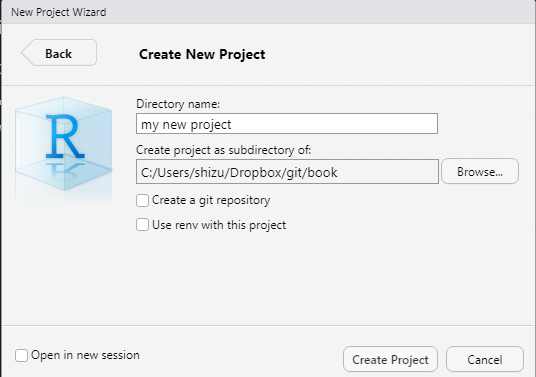
\includegraphics[width=0.4\linewidth]{images/project3} 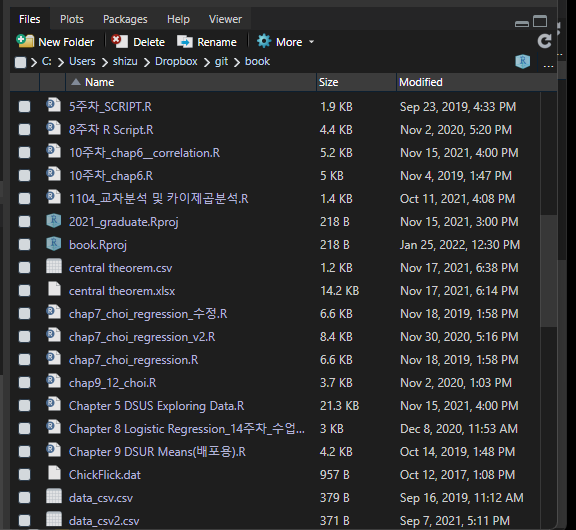
\includegraphics[width=0.4\linewidth]{images/project4} \caption{R prject 생성}\label{fig:unnamed-chunk-19}
\end{figure}

\textbf{work space 설정 방식}

두번째는 간단하게 나의 로컬 디렉토리(내컴퓨터안의 폴더)를 지정하는 방식이다. 간단한 작업을 수행할때 사용한다. 강력한 권고에도 불구하고 간단한 방식을 쓰고 싶은 사람들은 아래의 코드를 참고하라. (하지 말라는 뜻)
* getwd()를 실행하면 현재 working directory를 보여준다.
* setwd()를 실행하면 괄호안의 경로의 폴더가 working directory로 지정된다. 내가 작성한 R script나 output이 이 폴더에 저장됨을 뜻한다. 또한 working directory안의 파일들은 별도의 경로를 지정하지 않아도 파일이름만 쓰면 알아서 R이 인지한다.

\begin{Shaded}
\begin{Highlighting}[]
\FunctionTok{getwd}\NormalTok{()}
\FunctionTok{setwd}\NormalTok{(}\StringTok{"C:}\SpecialCharTok{\textbackslash{}\textbackslash{}}\StringTok{Users}\SpecialCharTok{\textbackslash{}\textbackslash{}}\StringTok{Owner}\SpecialCharTok{\textbackslash{}\textbackslash{}}\StringTok{Documents}\SpecialCharTok{\textbackslash{}\textbackslash{}}\StringTok{new"}\NormalTok{) }
\end{Highlighting}
\end{Shaded}

\hypertarget{uxb370uxc774uxd130-uxbd88uxb7ecuxc624uxae30}{%
\subsection{데이터 불러오기}\label{uxb370uxc774uxd130-uxbd88uxb7ecuxc624uxae30}}

패키지 설치가 완료되었다면 데이터를 불러와보자. 엑셀, txt, spss 파일 등 외부데이터를 불러오기 위해서는 가져오기(import)를 실행해야 한다. 데이터를 불러온다는 뜻은 외부데이터를 불러와서 R의 dataframe으로 재저장을 한다는 것을 의미한다. 대표적인 import 명령어는 다음과 같다.

\begin{itemize}
\tightlist
\item
  read.table()은 엑셀파일(.csv)을 불러올때 활용한다. 일반적인 엑셀파일 확장자명은 xlsx이지만, 이 파일형식을 불러오면 에러가 많다. 쉼표로 셀이 구분되는 .csv 파일로 재저장하여 불러오기를 하자. .xlsx를 불러오는 명령어도 따로 있지만 개인적으로 추천하지는 않는다.
\item
  read.spss()은 spss로 저장된 파일(.sav)을 불러올때 활용한다.
\item
  read.delim()은 텍스트파일(.dat)을 불러올때 활용한다.
\item
  데이터를 불러올때는 반드시 옵션을 잘 지정해두어야 한다. 1번째 행(row)이 머릿행(이름, 성별 등 변수명)인 경우에는 header=T, 구분자가 쉼표일때는 sep=``,''의 옵션 등을 사용하도록 하자.
\item
  spss파일의 경우 변수별 라벨(예: 남자=1, 여자=2)를 살리는 옵션(use.value.labels=T)이 있다. 필요에 따라 활용하라
\end{itemize}

아래의 코드를 좀더 자세히 살펴보자. 첫번째 코드는 나의 프로젝트 또는 작업공간안에 있는 data\_csv.csv파일을 불러와서 data\_csv라는 데이터 프레임 객체를 생성하라는 뜻이다. 마찬가지로 두번째 코드는 spss 파일을 불러오는 코드이다.
개인적으로는 거의 모든 파일을 csv 파일 형태로 전환하여 R에서 import하는 것을 추천한다. spss 등의 파일은 잡다한 정보들이 많이 붙어있어서 간혹 꼬이거나 행/열이 밀리는 경우가 존재한다. 만일 내가 spss 파일만 갖고 있다면 해당 패키지 -\textgreater{} 다른이름으로 저장을 누르고 저장방식을 csv로 바꾸는 것이 좋다.

\begin{Shaded}
\begin{Highlighting}[]
\NormalTok{data\_csv }\OtherTok{\textless{}{-}} \FunctionTok{read.table}\NormalTok{(}\StringTok{"data\_csv.csv"}\NormalTok{, }\AttributeTok{header =}\NormalTok{ T, }\AttributeTok{sep=}\StringTok{","}\NormalTok{) }
\NormalTok{data\_spss }\OtherTok{\textless{}{-}} \FunctionTok{read.spss}\NormalTok{(}\StringTok{"data\_sav.sav"}\NormalTok{, }\AttributeTok{use.value.labels=}\NormalTok{T, }\AttributeTok{to.data.frame=}\NormalTok{T)}
\end{Highlighting}
\end{Shaded}

\hypertarget{dplyr-uxd328uxd0a4uxc9c0uxc758-uxc774uxd574}{%
\section{dplyr 패키지의 이해}\label{dplyr-uxd328uxd0a4uxc9c0uxc758-uxc774uxd574}}

앞서서 데이터 전처리는 크게 두가지 단계 1) untidy한 데이터를 tidy 데이터로 만들기, 2) 데이터의 변형(연구목적에 맞게 데이터의 관측치 및 변수를 삭제, 조합하는 것)으로 나뉜다고 설명하였다. 이 장에서는 먼저 데이터의 변형에 대해 다루도록 하겠다. 그 이유는 untidy 데이터를 다루는 것이 더 높은 난이도이기 때문이다. 먼저 데이터 변형을 손쉽게 하는 수준에 오르게 되면, 그 다음 tidy화에 대해 배우는게 좋다. 다시말하면 이 챕터에서는 행에는 관측치가, 열에는 변수가 들어있는 데이터를 연구 목적에 맞게 변형하는것에 초점을 맞추도록 하겠다.

데이터 전처리 과정에서 주로 사용할 패키지는 dplyr다. tidyverse패키지 안에 들어있는 패키지로 단독설치도 가능하다. dplyr의 강점은 다음과 같다.

\begin{itemize}
\tightlist
\item
  R의 내장함수보다 직관적인 명령어 구조를 갖고 있다.
\item
  R보다 복잡한 자료변형이 가능하다.
\item
  chain operator(\%\%)를 사용하여 코드를 심플하게 짤 수 있다.
\end{itemize}

\hypertarget{chain-operator}{%
\subsection{chain operator}\label{chain-operator}}

먼저 chain operator에 대해 이해하면 dplyr의 강점을 십분 이해할 수 있다. 남이 짜둔 코드를 보다보면 마치 에러메시지와 같은 형태의 \%\textgreater\% 가 자주 등장한다. \%\textgreater\% 은 chain operator라 불리며 ``and then''의 문법과 같은 의미로 사용된다. 원래 R의 기본 코드는 괄호()가 이 기능을 수행한다.
빠른 이해를 위해 다음과 같은 짧은 코드를 살펴보자. x라는 객체를 만들고, 이 안에 30,20,10,0이라는 4개의 값을 지정한다. 만일 객체 x의 절대값(abs)을 구하고, 4개의 절대값의 평균값을 구한다음(mean), 다시 이 평균값의 제곱근(sqrt)을 구하고 싶다면 아래와 같이 코드를 짜야한다. 결국 괄호의 가장 안쪽부터 바깥쪽 까지 and then의 문법으로 계산이 이루어지는 것이다. 절대값을 구하고 and then 평균값을 구하고 and then 제곱근을 구하라는 명령이 sqrt(mean(abs()))의 코드로 구현된다.

\begin{Shaded}
\begin{Highlighting}[]
\NormalTok{x}\OtherTok{\textless{}{-}}\FunctionTok{c}\NormalTok{(}\DecValTok{30}\NormalTok{, }\DecValTok{20}\NormalTok{, }\DecValTok{10}\NormalTok{, }\DecValTok{0}\NormalTok{)}
\FunctionTok{sqrt}\NormalTok{(}\FunctionTok{mean}\NormalTok{(}\FunctionTok{abs}\NormalTok{(x)))}
\end{Highlighting}
\end{Shaded}

문제는 코드가 조금만 복잡해져도 괄호 갯수 등의 실수가 자주 발생한다는 것이다. 또한 가장 나중에 수행해야할 명령이 가장 먼저 코딩되야하기 때문에 직관적으로도 이해가 쉽지 않다. chain operator는 이러한 R코드의 문법구조를 좀더 직관적으로 바꾸는 역할을 한다. 위의 코드를 chain operator를 활용해서 바꿔보면 아래와 같다

\begin{Shaded}
\begin{Highlighting}[]
\NormalTok{x }\SpecialCharTok{\%\textgreater{}\%} 
  \FunctionTok{abs}\NormalTok{() }\SpecialCharTok{\%\textgreater{}\%} 
  \FunctionTok{mean}\NormalTok{() }\SpecialCharTok{\%\textgreater{}\%} 
  \FunctionTok{sqrt}\NormalTok{()}
\end{Highlighting}
\end{Shaded}

위의 코드에서 chain operator를 and then으로 바꾸어보면 마치 구어로 설명하듯이 편안하게 코드를 짤수 있다는 점을 확인할 수 있다. X를 가지고 와서 and then 절대값을 구하고, and then 평균값을 구하고, and then 제곱근값을 구하라는 뜻이다. chain operator는 코드가 복잡해지고, ggplot2 등을 활용하여 그래프를 그릴 때 강점이 잘 드러난다. 앞으로 이 책에서는 chain operator를 최대한 활용하여 코드를 설명할 예정이다. 다만 dplyr 패키지가 설치(install)되고 실행(library)된 상태에서만 chain operator가 정상적으로 실행된다는 점을 주의하자.

\hypertarget{dplyruxc758-uxc8fcuxc694-uxae30uxb2a5}{%
\section{dplyr의 주요 기능}\label{dplyruxc758-uxc8fcuxc694-uxae30uxb2a5}}

지금부터 dplyr의 가장 기본적이고 대표적인 기능을 하나하나 알아보도록 하겠다.

\hypertarget{filter}{%
\subsection{filter}\label{filter}}

filter 함수는 특정한 행(row)을 선택하는 기능이다. 시각적으로 생각하면 데이터를 횡의 방향으로 절단 또는 선택하는 기능이다. 예를 들어 데이터 중에 취업한 사람의 케이스만 선택하고 싶다면 filter 함수를 쓰면 된다.

코드 시현에 앞서서 R에 내장된 데이터를 불러와보자. R에는 연구자가 코드를 연습해볼 수 있는 다양한 종류의 데이터가 많이 있다. 여기서는 nycflights13이라는 데이터를 사용해보겠다. 이 데이터는 뉴욕공항에 1년동안 이륙/착륙한 비행기의 각종 정보가 담겨있다. 데이터를 불러오기 위해서는 nycflights13이라는 패키지를 설치하고 실행하면 된다.

\begin{Shaded}
\begin{Highlighting}[]
\FunctionTok{install.packages}\NormalTok{(}\StringTok{"nycflights13"}\NormalTok{, }\AttributeTok{repos =} \StringTok{"http://cran.us.r{-}project.org"}\NormalTok{)}
\DocumentationTok{\#\# package \textquotesingle{}nycflights13\textquotesingle{} successfully unpacked and MD5 sums checked}
\DocumentationTok{\#\# }
\DocumentationTok{\#\# The downloaded binary packages are in}
\DocumentationTok{\#\#  C:\textbackslash{}Users\textbackslash{}shizu\textbackslash{}AppData\textbackslash{}Local\textbackslash{}Temp\textbackslash{}Rtmp6XYOs5\textbackslash{}downloaded\_packages}
\FunctionTok{library}\NormalTok{(nycflights13)}
\DocumentationTok{\#\# Warning: 패키지 \textquotesingle{}nycflights13\textquotesingle{}는 R 버전 4.1.3에서 작성되었습니다}
\FunctionTok{head}\NormalTok{(flights) }\CommentTok{\# head 자료 수개를 보여줌}
\DocumentationTok{\#\# \# A tibble: 6 x 19}
\DocumentationTok{\#\#    year month   day dep\_time sched\_dep\_time dep\_delay arr\_time sched\_arr\_time}
\DocumentationTok{\#\#   \textless{}int\textgreater{} \textless{}int\textgreater{} \textless{}int\textgreater{}    \textless{}int\textgreater{}          \textless{}int\textgreater{}     \textless{}dbl\textgreater{}    \textless{}int\textgreater{}          \textless{}int\textgreater{}}
\DocumentationTok{\#\# 1  2013     1     1      517            515         2      830            819}
\DocumentationTok{\#\# 2  2013     1     1      533            529         4      850            830}
\DocumentationTok{\#\# 3  2013     1     1      542            540         2      923            850}
\DocumentationTok{\#\# 4  2013     1     1      544            545        {-}1     1004           1022}
\DocumentationTok{\#\# 5  2013     1     1      554            600        {-}6      812            837}
\DocumentationTok{\#\# 6  2013     1     1      554            558        {-}4      740            728}
\DocumentationTok{\#\# \# ... with 11 more variables: arr\_delay \textless{}dbl\textgreater{}, carrier \textless{}chr\textgreater{}, flight \textless{}int\textgreater{},}
\DocumentationTok{\#\# \#   tailnum \textless{}chr\textgreater{}, origin \textless{}chr\textgreater{}, dest \textless{}chr\textgreater{}, air\_time \textless{}dbl\textgreater{}, distance \textless{}dbl\textgreater{},}
\DocumentationTok{\#\# \#   hour \textless{}dbl\textgreater{}, minute \textless{}dbl\textgreater{}, time\_hour \textless{}dttm\textgreater{}}
\NormalTok{flight\_df }\OtherTok{\textless{}{-}}\FunctionTok{data.frame}\NormalTok{(flights)}\CommentTok{\#data frame으로 변환}
\FunctionTok{str}\NormalTok{(flight\_df)}
\DocumentationTok{\#\# \textquotesingle{}data.frame\textquotesingle{}:    336776 obs. of  19 variables:}
\DocumentationTok{\#\#  $ year          : int  2013 2013 2013 2013 2013 2013 2013 2013 2013 2013 ...}
\DocumentationTok{\#\#  $ month         : int  1 1 1 1 1 1 1 1 1 1 ...}
\DocumentationTok{\#\#  $ day           : int  1 1 1 1 1 1 1 1 1 1 ...}
\DocumentationTok{\#\#  $ dep\_time      : int  517 533 542 544 554 554 555 557 557 558 ...}
\DocumentationTok{\#\#  $ sched\_dep\_time: int  515 529 540 545 600 558 600 600 600 600 ...}
\DocumentationTok{\#\#  $ dep\_delay     : num  2 4 2 {-}1 {-}6 {-}4 {-}5 {-}3 {-}3 {-}2 ...}
\DocumentationTok{\#\#  $ arr\_time      : int  830 850 923 1004 812 740 913 709 838 753 ...}
\DocumentationTok{\#\#  $ sched\_arr\_time: int  819 830 850 1022 837 728 854 723 846 745 ...}
\DocumentationTok{\#\#  $ arr\_delay     : num  11 20 33 {-}18 {-}25 12 19 {-}14 {-}8 8 ...}
\DocumentationTok{\#\#  $ carrier       : chr  "UA" "UA" "AA" "B6" ...}
\DocumentationTok{\#\#  $ flight        : int  1545 1714 1141 725 461 1696 507 5708 79 301 ...}
\DocumentationTok{\#\#  $ tailnum       : chr  "N14228" "N24211" "N619AA" "N804JB" ...}
\DocumentationTok{\#\#  $ origin        : chr  "EWR" "LGA" "JFK" "JFK" ...}
\DocumentationTok{\#\#  $ dest          : chr  "IAH" "IAH" "MIA" "BQN" ...}
\DocumentationTok{\#\#  $ air\_time      : num  227 227 160 183 116 150 158 53 140 138 ...}
\DocumentationTok{\#\#  $ distance      : num  1400 1416 1089 1576 762 ...}
\DocumentationTok{\#\#  $ hour          : num  5 5 5 5 6 5 6 6 6 6 ...}
\DocumentationTok{\#\#  $ minute        : num  15 29 40 45 0 58 0 0 0 0 ...}
\DocumentationTok{\#\#  $ time\_hour     : POSIXct, format: "2013{-}01{-}01 05:00:00" "2013{-}01{-}01 05:00:00" ...}
\end{Highlighting}
\end{Shaded}

nycflights13을 실행시키면 flights라는 데이터를 사용할 수 있게 된다. 가장 먼저 데이터의 구조를 판단하고, dataframe으로 변환하는 작업이 필요하다.

\begin{itemize}
\tightlist
\item
  head()는 자료의 첫 행 6개와 첫 열 6개를 보여준다. 출력결과를 살펴보면 year, month, day, dep\_time 등의 변수에 정수형 자료들이 예시로 제시되어 있다.
\item
  data.frame()은 tibble의 자료 구조를 dataframe으로 바꾸는 명령어이다.
\item
  str()은 데이터 프레임의 구조(행과 열의 갯수, 변수명, 변수의 자료 유형 등)를 보여준다.
\end{itemize}

dataframe으로 변환한 flight\_df라는 객체는 R studio의 오른쪽 상단 environment창에 뜨게 된다. 이를 더블 클릭하게 되면 script 창에 우리에게 친숙한 데이터시트가 뜬다. 콘솔창에 나타난 결과를 보면 flight\_df는 336776개의 관측치(=행의 갯수가 336,776개)와 19개의 변수(=열의 갯수가 19개)인 것을 확인할 수 있다. 대부분의 변수가 정수 또는 수치형 자료이고, 출발지(origin), 도착지(dest) 등은 문자형 변수이다.

본격적으로 filter 함수에 대해 알아보자. filter는 자료를 횡으로 자르는 것이다. 바꿔말하면 어떠한 변수가 특정값인 관측치만 선택하는 것이다. 예를 들어 month가 1인 자료만 선택하고 싶다면 month=1로 필터링을 하는 것이다.

\begin{Shaded}
\begin{Highlighting}[]
\DocumentationTok{\#\#month=2인 자료만 필터링}
\NormalTok{flight\_df }\SpecialCharTok{\%\textgreater{}\%} 
  \FunctionTok{filter}\NormalTok{(month}\SpecialCharTok{==}\DecValTok{2}\NormalTok{) }\SpecialCharTok{\%\textgreater{}\%}
\DocumentationTok{\#\#month=2 or day=1 자료만 필터링}
\NormalTok{flight\_df }\SpecialCharTok{\%\textgreater{}\%} 
  \FunctionTok{filter}\NormalTok{(month}\SpecialCharTok{==}\DecValTok{2} \SpecialCharTok{|}\NormalTok{ day}\SpecialCharTok{==}\DecValTok{1}\NormalTok{) }\SpecialCharTok{\%\textgreater{}\%}  \CommentTok{\#shift+\textbackslash{}}
\DocumentationTok{\#\#month=2 and day=1 자료만 필터링}
\NormalTok{flight\_df }\SpecialCharTok{\%\textgreater{}\%} 
  \FunctionTok{filter}\NormalTok{(month}\SpecialCharTok{==}\DecValTok{2}\NormalTok{, day}\SpecialCharTok{==}\DecValTok{1}\NormalTok{) }\SpecialCharTok{\%\textgreater{}\%}  \CommentTok{\#쉼표나 \& 모두 사용 가능}

\DocumentationTok{\#\#month=2가 아닌 자료만 필터링}
\NormalTok{flight\_df }\SpecialCharTok{\%\textgreater{}\%} 
  \FunctionTok{filter}\NormalTok{(month}\SpecialCharTok{!=}\DecValTok{2}\NormalTok{) }\SpecialCharTok{\%\textgreater{}\%}  \CommentTok{\#느낌표는 not의 의미}
\DocumentationTok{\#\#month가 5이상인 자료만 필터링}
\NormalTok{flight\_df }\SpecialCharTok{\%\textgreater{}\%} 
  \FunctionTok{filter}\NormalTok{(month }\SpecialCharTok{\textgreater{}=}\DecValTok{5}\NormalTok{) }\SpecialCharTok{\%\textgreater{}\%}  
\DocumentationTok{\#\#month가 5, 7, 10인 자료만(복수의 조건) 필터링}
\NormalTok{flight\_df }\SpecialCharTok{\%\textgreater{}\%} 
  \FunctionTok{filter}\NormalTok{(month }\SpecialCharTok{\%in\%} \FunctionTok{c}\NormalTok{(}\DecValTok{5}\NormalTok{,}\DecValTok{7}\NormalTok{,}\DecValTok{10}\NormalTok{))}
\DocumentationTok{\#\#na 값 표시 또는 제거 해서 필터링}
\NormalTok{flight\_df }\SpecialCharTok{\%\textgreater{}\%} 
  \FunctionTok{filter}\NormalTok{(}\FunctionTok{is.na}\NormalTok{(month)) }\CommentTok{\#na인 row만 표시}
\NormalTok{flight\_df }\SpecialCharTok{\%\textgreater{}\%} 
  \FunctionTok{filter}\NormalTok{(}\SpecialCharTok{!}\FunctionTok{is.na}\NormalTok{(month)) }\CommentTok{\#na가 아닌 row만 표시}
\end{Highlighting}
\end{Shaded}

\begin{itemize}
\tightlist
\item
  주로 equal(==), and(\&), or(\textbar), not equal(!=), greater than or equal to(\textgreater=), greater than(\textgreater), less than(\textless), less than or equal to(\textless=) 를 사용하여 관측치를 필터링한다.
\item
  na값만 필터링하기 위해서는 is.na(), na값을 제외하여 필터링하기 위해서는 !is.na()를 사용한다.
\item
  복수의 조건을 사용하여 필터링하기 위해서는 \%in\% c()의 구문을 사용한다.
\item
  dplyr의 모든 명령어는 tibble을 활용하여 임시적으로 데이터를 변형한다. 다시 말해 원래의 dataframe을 변형시키지는 않는다. 따라서 별도의 데이터 셋으로 저장하는 절차가 필요하다.
\item
  만일 변형한 데이터를 저장하고 싶다면 새로운 데이터 프레임 또는 기존의 데이터 프레임에 저장하는 명령어를 추가해야한다. 저장은 아주 간단하게 \textless- 를 사용하면된다. summary 명령어를 통해 데이터 변형이 잘 이루어졌는지 꼭 확인이 필요하다.
\end{itemize}

\begin{Shaded}
\begin{Highlighting}[]
\NormalTok{filter\_df2 }\OtherTok{\textless{}{-}}
\NormalTok{  flight\_df }\SpecialCharTok{\%\textgreater{}\%} 
  \FunctionTok{filter}\NormalTok{(month }\SpecialCharTok{\%in\%} \FunctionTok{c}\NormalTok{(}\DecValTok{5}\NormalTok{,}\DecValTok{7}\NormalTok{,}\DecValTok{10}\NormalTok{))}
\FunctionTok{summary}\NormalTok{(filter\_df2}\SpecialCharTok{$}\NormalTok{month)}
\end{Highlighting}
\end{Shaded}

\hypertarget{select}{%
\subsection{select}\label{select}}

select는 특정 변수(열, column)을 선택하는 명령어이다. filter와는 정반대로 dataset을 종으로 절단하는 기능이다. 1차 자료를 연구 목적에 맞게 간추릴때 필요없는 변수를 삭제하거나 필요한 변수만을 선택해야하는 경우가 있다. 이때 select가 유용하게 사용된다.

\begin{itemize}
\tightlist
\item
  select() 명령어의 괄호안에 선택할 변수명을 쉼표로 이어가며 작성하는 방식이 일반적이다.
\item
  콜론(:)은 연속적인 변수를 선택할때 사용한다.
\item
  느낌표(!)는 해당 변수를 제외한 변수들을 선택할때 사용한다. 복수의 변수를 제외하고 싶다면 c()로 연결하면 된다.
  *startsWith, endsWith, one\_of를 활용하면 변수명을 조합하여 선택도 가능하다.
\end{itemize}

\begin{Shaded}
\begin{Highlighting}[]
\CommentTok{\#month, day 변수만 선택}
\NormalTok{flight\_df }\SpecialCharTok{\%\textgreater{}\%}
  \FunctionTok{select}\NormalTok{(month, day)}
\CommentTok{\#year에서 day까지의 변수만 선택}
\NormalTok{flight\_df }\SpecialCharTok{\%\textgreater{}\%}
  \FunctionTok{select}\NormalTok{(year}\SpecialCharTok{:}\NormalTok{day) }
\CommentTok{\#year에서 day까지의 변수만 제외해서 선택}
\NormalTok{flight\_df }\SpecialCharTok{\%\textgreater{}\%}
  \FunctionTok{select}\NormalTok{(}\SpecialCharTok{!}\NormalTok{ year}\SpecialCharTok{:}\NormalTok{day)}
\CommentTok{\#복수의 변수를 제외하고 싶은 경우 {-}c()를 사용}
\NormalTok{flight\_df }\SpecialCharTok{\%\textgreater{}\%}
  \FunctionTok{select}\NormalTok{(}\SpecialCharTok{{-}}\FunctionTok{c}\NormalTok{(year, month)) }
\CommentTok{\#dep이라는 단어로 시작하는 변수들 선택}
\NormalTok{flight\_df }\SpecialCharTok{\%\textgreater{}\%} 
  \FunctionTok{select}\NormalTok{(}\FunctionTok{startsWith}\NormalTok{(}\StringTok{"dep"}\NormalTok{))}
\CommentTok{\#time이라는 단어로 끝나는 변수들 선택}
\NormalTok{flight\_df }\SpecialCharTok{\%\textgreater{}\%} 
  \FunctionTok{select}\NormalTok{(}\FunctionTok{endsWith}\NormalTok{(}\StringTok{"time"}\NormalTok{))}
\CommentTok{\#time 또는 delay 중 하나라도 포함되어 있는 변수들 선택}
\NormalTok{flight\_df }\SpecialCharTok{\%\textgreater{}\%} 
  \FunctionTok{select}\NormalTok{(}\FunctionTok{one\_of}\NormalTok{(}\FunctionTok{c}\NormalTok{(}\StringTok{"time"}\NormalTok{, }\StringTok{"delay"}\NormalTok{)))}
\end{Highlighting}
\end{Shaded}

\hypertarget{arrange}{%
\subsection{arrange}\label{arrange}}

arrange는 특정한 변수를 기준으로 정렬을 할때 사용하는 명령어이다. 오름차순과 내림차순, 그리고 두개 이상의 변수를 활용한 2차 이상의 정렬도 가능하다.

\begin{Shaded}
\begin{Highlighting}[]

\DocumentationTok{\#\#month, day 순으로 오름차순}
\NormalTok{flight\_df }\SpecialCharTok{\%\textgreater{}\%}
  \FunctionTok{arrange}\NormalTok{(month, day) }
\DocumentationTok{\#\#month는 오름차순, day는 내림차순}
\NormalTok{flight\_df }\SpecialCharTok{\%\textgreater{}\%}
  \FunctionTok{arrange}\NormalTok{(month, }\SpecialCharTok{{-}}\NormalTok{day) }
\NormalTok{flight\_df }\SpecialCharTok{\%\textgreater{}\%}
  \FunctionTok{arrange}\NormalTok{(month, }\FunctionTok{desc}\NormalTok{(day))}
\DocumentationTok{\#\#month, day 순으로 내림차순}
\NormalTok{flight\_df }\SpecialCharTok{\%\textgreater{}\%}
  \FunctionTok{arrange}\NormalTok{(}\SpecialCharTok{{-}}\NormalTok{month, }\SpecialCharTok{{-}}\NormalTok{day) }
\NormalTok{flight\_df }\SpecialCharTok{\%\textgreater{}\%}
  \FunctionTok{arrange}\NormalTok{(}\FunctionTok{desc}\NormalTok{(month), }\FunctionTok{desc}\NormalTok{(day))}
\end{Highlighting}
\end{Shaded}

\hypertarget{mutate}{%
\subsection{mutate}\label{mutate}}

mutate는 기존의 변수를 활용하여 새로운 변수를 만드는 명령어이다. 보통 이런 변수를 파생변수(derived variables)라고 부른다. 예를 들어 소요시간(time)과 거리(distance)라는 원변수가 있다면, 거리/소요시간으로 속력(speed)이라는 새로운 변수를 만드는 방식이다. 또는 x1\textasciitilde x5의 5개의 문항의 평균값을 의미하는 새로운 변수를 만드는 것도 mutate 명령어를 활용할 수 있다. mutate는 크게 두가지 방식이 있다. 첫째는 덧셈, 뺄셈, 곱셈, 나눗셈, 로그, 제곱근 등 다양한 연산을 통해 파생변수를 만드는 방식, 둘째는 ifelse 구문을 활용하여 조건을 만족하는 경우 특정 값을 부여하는 방식(dummy coding) 이다.

\begin{itemize}
\tightlist
\item
  mutate(새로운변수명=수식 또는 논리식)의 구조를 띈다.
\item
  연산의 경우 +, -, *, /, log, sqrt 등 대부분의 연산자를 활용하여 수식을 작성한다.
\item
  더미 코딩을 위해 ifelse를 사용하는 경우 mutate(새로운변수명 = ifelse(조건, TRUE값, FALSE값))의 구조를 띈다.
\item
  mutate의 경우 반드시 새로운 데이터 프레임으로 저장하는 명령어(-\textgreater newdataframename)를 추가하는 것이 필요하다.
\item
  만일 기존 변수를 삭제(drop)하고 싶은 경우에는 mutate대신에 transmute를 사용한다.
\item
  변수의 이름을 바꾸고 싶다면 rename(새로운변수=기존변수)를 사용한다.
\end{itemize}

\begin{Shaded}
\begin{Highlighting}[]
\CommentTok{\#평균 또는 ratio로 연산하여 새로운 변수를 생성}
\NormalTok{flight\_df }\SpecialCharTok{\%\textgreater{}\%}
  \FunctionTok{mutate}\NormalTok{(}\AttributeTok{mean\_distance=}\NormalTok{distance}\SpecialCharTok{/}\NormalTok{hour, }
         \AttributeTok{ratio\_delay=}\NormalTok{arr\_delay}\SpecialCharTok{/}\NormalTok{(hour}\SpecialCharTok{*}\DecValTok{60}\SpecialCharTok{+}\NormalTok{minute)) }\OtherTok{{-}\textgreater{}}\NormalTok{ flght\_df\_mutate}
\CommentTok{\#ifelse를 활용하여 category변수 생성, ifelse(조건, 조건이 true일때, 조건이 false)}
\NormalTok{flight\_df }\SpecialCharTok{\%\textgreater{}\%}
  \FunctionTok{mutate}\NormalTok{(}\AttributeTok{arr\_delay\_group=}\FunctionTok{ifelse}\NormalTok{(arr\_delay}\SpecialCharTok{\textgreater{}}\DecValTok{0}\NormalTok{, }\StringTok{"delay"}\NormalTok{, }\StringTok{"no delay"}\NormalTok{)) }\OtherTok{{-}\textgreater{}}\NormalTok{flight\_df\_mutate}
\CommentTok{\#사용한 변수를 삭제하고 새로운 변수만 남기는 경우}
\NormalTok{flight\_df }\SpecialCharTok{\%\textgreater{}\%} 
  \FunctionTok{transmute}\NormalTok{(}\AttributeTok{total\_min=}\NormalTok{hour}\SpecialCharTok{*}\DecValTok{60}\SpecialCharTok{+}\NormalTok{minute) }\OtherTok{{-}\textgreater{}}\NormalTok{ flight\_df\_mutate}
\end{Highlighting}
\end{Shaded}

\hypertarget{group_byuxc640-summarise}{%
\subsection{group\_by와 summarise}\label{group_byuxc640-summarise}}

데이터의 전처리 단계에서는 집단별 평균값이나 빈도를 비교해야 하는 경우가 종종 발생한다. 예를 들어 성별에 따라 특정변수에 값에 차이가 있는지? 연도에 따라 평균값이 어떻게 변하는지? 학년별로 결측치 빈도가 어떻게 다른지? 등이 이에 해당된다.
이러한 상황을 시각적으로 생각해보면 데이터가 일종의 축소 또는 요약되는 것을 쉽게 이해할 수 있다.
예를 들어 남성 50명, 여성 50명의 IQ, GPA, 학습시간의 데이터가 있다고 생각해보자. dataframe의 형태로 생각해보면 100개의 행(row, 관측치 갯수)과 4개의 열(column, 변수의 갯수)의 100x4의 매트릭스일 것이다. 만일 성별에 따라 IQ, GPA, 학습시간의 평균값을 비교하고 싶다면 2개의 행(group의 수)과 3개의 열(변수의 수)의 2x3의 새로운 매트릭스로 결과가 제시된다.
dplyr는 이러한 과정을 group\_by(집단으로 데이터를 쪼개서 비교하고)와 summarise(데이터를 요약)의 두개의 명령어 조합으로 수행한다. 통상 group\_by와 summarise는 짝꿍처럼 뗄레야 뗄수없는 사이로 표현된다. 왜냐하면 summarise 없이 group\_by는 의미가 거의 없기 때문이다.

다시 flight 데이터로 돌아와보자. group\_by 변수로 쓸만한 것들은 무엇이 있을까? 연속적인 수치형 변수보다는 factor 변수나 값의 갯수에 제한이 있는 수치형 자료가 group 변수로 적절하다는 것을 직감했을 거라 생각한다. 왜냐하면 출발시간(dep\_time)처럼 수천개의 값을 가진 연속형 변수들을 기준으로 집단을 구분하는 것은 의미가 없기 때문이다.
앞서 mutate에서 도착 시간 지연여부(arr\_delay\_group)를 만들어낸 것을 기억하자.
도착시간보다 지연 도착한 비행기는 delay, 그렇지 않은 경우는 no delay로 변형을 시켰다. 먼저 summary 명령어를 활용하여 arr\_delay\_group 변수의 현황을 살펴보자. 어떤 변수의 빈도를 확인하고 싶다면 r 내장함수인 table()을 써도 좋지만, dplyr에서 제공하는 count() 함수가 훨씬 간편하다. 아래 코드를 보면 (1)mutate1\_flihgt\_df 데이터프레임을 불러와서, (2) arr\_delay\_group 변수의 빈도를 count 하라는 뜻이다.

\begin{Shaded}
\begin{Highlighting}[]
\NormalTok{mutate1\_flight\_df }\SpecialCharTok{\%\textgreater{}\%} 
  \FunctionTok{count}\NormalTok{(arr\_delay\_group)}
\DocumentationTok{\#\# Error in count(., arr\_delay\_group): 객체 \textquotesingle{}mutate1\_flight\_df\textquotesingle{}를 찾을 수 없습니다}
\end{Highlighting}
\end{Shaded}

결과를 살펴보면 delay인 사례는 133,004개, no delay는 194,342개, 그리고 na값이 9,430개이다. 만일 na값을 그대로 두고 group\_by와 summarise 함수를 적용하면 어떻게 될까? 아래 코드는 arr\_delay\_group별로 arr\_delay 변수의 최대값(max), 최솟값(min), 평균값(mean), 중위값(median), 4분위값(quantile)을 산출하라는 뜻이다.

\begin{itemize}
\tightlist
\item
  group\_by는 반드시 summarise 전에 코드가 작성되어야 한다.
\item
  summrise는 새로운 tibble을 만들어내는 방식이다. 다시이야기하면 observation x variables의 데이터 프레임을 활용해서 변수 x 통계값의 새로운 요약된 데이터 프레임을 만들어내는 방식이다. 따라서 각 통계값에 해당되는 일종의 변수명을 지정해주는 것이 필요하다.
\item
  mean(x,na.rm=TRUE) : 결측값제외하고 평균
\item
  median(x,na.rm=TRUE) : 중앙값
\item
  sd(x,na.rm=TRUE) : 표준편차
\item
  min(x,na.rm=TRUE) : 최솟값
\item
  max(x,na.rm=TRUE) : 최대값
\item
  IQR(x,na.rm=TRUE) : 사분위수 : Q3-Q1
\item
  sum(x,na.rm=TRUE) : 합
\item
  n() 관측치 개수 계산, x변수 입력 하지 않음
\item
  n\_disinct(x) : 중복없는 유일한 관측치 개수 계산
\end{itemize}

\begin{Shaded}
\begin{Highlighting}[]
\NormalTok{mutate1\_flight\_df }\SpecialCharTok{\%\textgreater{}\%} 
  \FunctionTok{group\_by}\NormalTok{(arr\_delay\_group) }\SpecialCharTok{\%\textgreater{}\%} 
  \FunctionTok{summarise}\NormalTok{(}\AttributeTok{max=}\FunctionTok{max}\NormalTok{(arr\_delay),}
            \AttributeTok{min=}\FunctionTok{min}\NormalTok{(arr\_delay), }
            \AttributeTok{mean=}\FunctionTok{mean}\NormalTok{(arr\_delay), }
            \AttributeTok{med=}\FunctionTok{median}\NormalTok{(arr\_delay), }
            \AttributeTok{per25=}\FunctionTok{quantile}\NormalTok{(arr\_delay, }\DecValTok{0}\NormalTok{,}\DecValTok{25}\NormalTok{))}
\DocumentationTok{\#\# Error in group\_by(., arr\_delay\_group): 객체 \textquotesingle{}mutate1\_flight\_df\textquotesingle{}를 찾을 수 없습니다}
\end{Highlighting}
\end{Shaded}

결과값을 살펴보면 no delay 집단의 경우 arr\_delay 값이 음수값을 가지기 때문에 통계값 역시 음수값을 갖는 것으로 확인되었다. 문제는 na 집단이다. na 집단을 제외하고 다시 summarise를 해보도록 하자. 앞에서 쓴 코드에 filter 명령어만 삽입하면 간단하게 해결된다. !is.na()가 na가 아닌 row만 표시하는 옵션임을 기억하자. 마지막으로 summarise 함수의 작동방식을 제대로 이해하기 위해 아웃풋을 final이라는 dataframe으로 별도로 저장해보자.

\begin{Shaded}
\begin{Highlighting}[]
\NormalTok{flight\_df }\SpecialCharTok{\%\textgreater{}\%}
  \FunctionTok{filter}\NormalTok{(}\SpecialCharTok{!}\FunctionTok{is.na}\NormalTok{(arr\_delay)) }\SpecialCharTok{\%\textgreater{}\%}  \CommentTok{\#na가 아닌 row만 표시}
  \FunctionTok{mutate}\NormalTok{(}\AttributeTok{arr\_delay\_group=}\FunctionTok{ifelse}\NormalTok{(arr\_delay}\SpecialCharTok{\textgreater{}}\DecValTok{0}\NormalTok{, }\StringTok{"delay"}\NormalTok{, }\StringTok{"no delay"}\NormalTok{)) }\SpecialCharTok{\%\textgreater{}\%} 
  \FunctionTok{group\_by}\NormalTok{(arr\_delay\_group) }\SpecialCharTok{\%\textgreater{}\%} 
  \FunctionTok{summarise}\NormalTok{(}\AttributeTok{max=}\FunctionTok{max}\NormalTok{(arr\_delay),}
            \AttributeTok{min=}\FunctionTok{min}\NormalTok{(arr\_delay), }
            \AttributeTok{mean=}\FunctionTok{mean}\NormalTok{(arr\_delay), }
            \AttributeTok{med=}\FunctionTok{median}\NormalTok{(arr\_delay), }
            \AttributeTok{per20=}\FunctionTok{quantile}\NormalTok{(arr\_delay, }\DecValTok{0}\NormalTok{,}\DecValTok{25}\NormalTok{),}
            \AttributeTok{n=}\FunctionTok{n}\NormalTok{())}\OtherTok{{-}\textgreater{}}\NormalTok{final}
\NormalTok{final}
\DocumentationTok{\#\# \# A tibble: 2 x 7}
\DocumentationTok{\#\#   arr\_delay\_group   max   min  mean   med per20      n}
\DocumentationTok{\#\#   \textless{}chr\textgreater{}           \textless{}dbl\textgreater{} \textless{}dbl\textgreater{} \textless{}dbl\textgreater{} \textless{}dbl\textgreater{} \textless{}dbl\textgreater{}  \textless{}int\textgreater{}}
\DocumentationTok{\#\# 1 delay            1272     1  40.3    21     1 133004}
\DocumentationTok{\#\# 2 no delay            0   {-}86 {-}16.0   {-}15   {-}86 194342}
\end{Highlighting}
\end{Shaded}

\hypertarget{uxb370uxc774uxd130-uxacb0uxd569uxd558uxae30}{%
\section{데이터 결합하기}\label{uxb370uxc774uxd130-uxacb0uxd569uxd558uxae30}}

연구를 진행하다보면 두개 이상의 데이터를 결합해야 하는 경우가 종종 발생한다. 시계열 데이터를 연결하는 것이 가장 대표적인 사례다. 또는 몇개의 변수를 더 추가하거나, 몇 개의 사례를 더 추가하는 등의 간단한 결합도 자주 발생한다. dplyr는 다양한 종류의 데이터 결합에 탁월한 기능을 갖고 있다. 혹자는 엑셀로 데이터를 붙이는 무모한 시도를 하는 경우가 있는데 대체로 많은 오류를 발생시킨다. 특히 데이터에 빈 구멍이 있는 경우에는 더욱 그러하다. 예를 들어 어떤 패널 데이터의 1차년도 자료와 2차년도 자료를 결합하는 상황을 생각해보자. 종단데이터의 경우 각 관측치(사례)를 연결하는 key 변수인 ID를 제공한다. 하지만 1차년도 자료와 2차년도 자료는 완전히 동일한 ID가 아닌 경우가 많다. 1차년도에는 응답하였지만 2차년도에는 응답하지 않은 사람은 어떻게 처리해야할까? 또 1차년도 자료와 2차년도 자료와 동일한 변수는 어떻게 drop 해야 할까? dplyr는 이러한 다양한 데이터 결합에 최적의 기능을 제공한다. 이 챕터에서는 아주 간단한 결합(단순히 coloums과 rows를 추가하는 형태)부터 복잡한 결합(두 자료의 교집합 또는 한자료의 여집합만 결합하는 형태 등)을 구분하여 설명해보도록 하겠다.

\hypertarget{bind_colsuxc640-bind_rowsuxb85c-uxb370uxc774uxd130-uxacb0uxd569uxd558uxae30}{%
\subsection{bind\_cols와 bind\_rows로 데이터 결합하기}\label{bind_colsuxc640-bind_rowsuxb85c-uxb370uxc774uxd130-uxacb0uxd569uxd558uxae30}}

bind 명령어는 말그대로 두개의 벡터를 결합하는 기능이다. 좀더 손쉬운 이해를 위해 간단한 데이터 셋 두개를 직접 만들어서 붙여보자. 2장을 복습할 겸 BTS 데이터를 다시 만들어보자. BTS 멤버 7명의(row 7개) 이름, 출생년도, 포지션의 3개의 변수(column 3개)로 구성되어 있는 bts1이라는 데이터 프레임을 생성해보았다. 다음으로는 각 멤버별 솔로곡의 이름을 문자형 변수로 지정한 bts2라는 데이터 프레임을 추가로 생성하였다. 두 데이터 프레임을 결합한다는 것은 변수를 한개 추가하는 것이기 때문에 bind\_cols의 명령어를 사용한다. 결합해야하는 2개 이상의 데이터 프레임 이름을 쉼표를 활용하여 연결시켜준다.

\begin{Shaded}
\begin{Highlighting}[]
\CommentTok{\#bts1 dataframe 만들기}
\NormalTok{btsname }\OtherTok{\textless{}{-}}\FunctionTok{c}\NormalTok{(}\StringTok{"RM"}\NormalTok{, }\StringTok{"Jin"}\NormalTok{, }\StringTok{"Suga"}\NormalTok{,}\StringTok{"Jhope"}\NormalTok{, }\StringTok{"Jimin"}\NormalTok{, }\StringTok{"V"}\NormalTok{, }\StringTok{"JK"}\NormalTok{)}
\NormalTok{btsyear }\OtherTok{\textless{}{-}}\FunctionTok{c}\NormalTok{(}\DecValTok{1994}\NormalTok{, }\DecValTok{1992}\NormalTok{, }\DecValTok{1993}\NormalTok{, }\DecValTok{1994}\NormalTok{, }\DecValTok{1995}\NormalTok{, }\DecValTok{1995}\NormalTok{, }\DecValTok{1997}\NormalTok{)}
\NormalTok{btsposition }\OtherTok{\textless{}{-}}\FunctionTok{c}\NormalTok{(}\StringTok{"rap"}\NormalTok{, }\StringTok{"vocal"}\NormalTok{, }\StringTok{"rap"}\NormalTok{, }\StringTok{"rap"}\NormalTok{, }\StringTok{"vocal"}\NormalTok{, }\StringTok{"vocal"}\NormalTok{,}\StringTok{"vocal"}\NormalTok{)}
\NormalTok{bts1 }\OtherTok{\textless{}{-}}\FunctionTok{data.frame}\NormalTok{(btsname, btsyear, btsposition, }\AttributeTok{stringsAsFactors =} \ConstantTok{FALSE}\NormalTok{)}
\CommentTok{\#bts2 dataframe 만들기}
\NormalTok{soloSong }\OtherTok{\textless{}{-}}\FunctionTok{c}\NormalTok{(}\StringTok{"her"}\NormalTok{, }\StringTok{"epiphany"}\NormalTok{, }\StringTok{"seesaw"}\NormalTok{, }\StringTok{"justDance"}\NormalTok{, }\StringTok{"serendipity"}\NormalTok{, }\StringTok{"singularity"}\NormalTok{, }\StringTok{"euphoria"}\NormalTok{)}
\NormalTok{bts2}\OtherTok{\textless{}{-}}\FunctionTok{data.frame}\NormalTok{(soloSong)}
\CommentTok{\#bts1과 bts2를 횡으로 결합하기 (변수추가)}
\FunctionTok{bind\_cols}\NormalTok{(bts1, bts2)}
\DocumentationTok{\#\#   btsname btsyear btsposition    soloSong}
\DocumentationTok{\#\# 1      RM    1994         rap         her}
\DocumentationTok{\#\# 2     Jin    1992       vocal    epiphany}
\DocumentationTok{\#\# 3    Suga    1993         rap      seesaw}
\DocumentationTok{\#\# 4   Jhope    1994         rap   justDance}
\DocumentationTok{\#\# 5   Jimin    1995       vocal serendipity}
\DocumentationTok{\#\# 6       V    1995       vocal singularity}
\DocumentationTok{\#\# 7      JK    1997       vocal    euphoria}
\end{Highlighting}
\end{Shaded}

결과를 살펴보면 bts1 데이터 프레임에 soloSong이라는 변수가 잘 결합되어 있는것을 볼 수 있다. 만일 새로 추가하는 변수에 missing 값이 있다면 어떻게 될까? NA가 포함되어 있는 bts3, bts4의 데이터 프레임을 추가로 생성하여 bind\_cols를 사용하여 결합해보았다. 결과에서 볼 수 있듯이 NA가 포함되어 잘 연결되어 있는 것을 볼 수 있다.

\begin{Shaded}
\begin{Highlighting}[]
\NormalTok{singularity }\OtherTok{\textless{}{-}}\FunctionTok{c}\NormalTok{(}\ConstantTok{NA}\NormalTok{, }\StringTok{"vocal"}\NormalTok{, }\ConstantTok{NA}\NormalTok{, }\ConstantTok{NA}\NormalTok{, }\StringTok{"vocal"}\NormalTok{, }\StringTok{"vocal"}\NormalTok{, }\StringTok{"vocal"}\NormalTok{)}
\NormalTok{tear }\OtherTok{\textless{}{-}}\FunctionTok{c}\NormalTok{(}\StringTok{"rap"}\NormalTok{, }\ConstantTok{NA}\NormalTok{, }\StringTok{"rap"}\NormalTok{, }\StringTok{"rap"}\NormalTok{, }\ConstantTok{NA}\NormalTok{, }\ConstantTok{NA}\NormalTok{, }\ConstantTok{NA}\NormalTok{)}
\NormalTok{bts3}\OtherTok{\textless{}{-}}\FunctionTok{data.frame}\NormalTok{(singularity)}
\NormalTok{bts4}\OtherTok{\textless{}{-}}\FunctionTok{data.frame}\NormalTok{(tear)}
\FunctionTok{bind\_cols}\NormalTok{(bts1, bts2, bts3, bts4)}\OtherTok{{-}\textgreater{}}\NormalTok{bts}
\end{Highlighting}
\end{Shaded}

bind\_cols를 사용할때 유의할 점과 강점은 다음과 같다.

\begin{itemize}
\tightlist
\item
  bind\_cols(dataframe1, dataframe 2,\ldots.)의 명령어 구조를 사용한다.
\item
  NA가 포함되어 있는 셀들은 이상없이 결합된다.
\item
  데이터 프레임의 행(rows)의 갯수가 서로 다르면 작동이 되지 않는다. 예를들어 bts1의 행의 갯수가 7개, bts2의 행의 갯수가 6개이면 결합되지 않는다.
\end{itemize}

두번째로 rows를 추가하는 방식은 bind\_rows를 사용한다. 이를 위해 제8의 멤버로 army를 추가해보도록 하겠다. 이름에만 army를 추가하고 나머지 변수에는 NA값을 할당하였다. bind\_rows 역시 bind\_cols와 유사하게 괄호안에 데이터프레임명을 쉼표로 연결하면 된다.

\begin{Shaded}
\begin{Highlighting}[]
\NormalTok{army }\OtherTok{\textless{}{-}}\FunctionTok{data.frame}\NormalTok{(}\AttributeTok{btsname=}\StringTok{"army"}\NormalTok{, }\AttributeTok{btsyear=}\ConstantTok{NA}\NormalTok{, }\AttributeTok{btsposition=}\ConstantTok{NA}\NormalTok{, }\AttributeTok{soloSong=}\ConstantTok{NA}\NormalTok{, }\AttributeTok{singularity=}\ConstantTok{NA}\NormalTok{, }\AttributeTok{tear=}\ConstantTok{NA}\NormalTok{)}
\FunctionTok{bind\_rows}\NormalTok{(bts, army)}
\DocumentationTok{\#\#   btsname btsyear btsposition    soloSong singularity tear}
\DocumentationTok{\#\# 1      RM    1994         rap         her        \textless{}NA\textgreater{}  rap}
\DocumentationTok{\#\# 2     Jin    1992       vocal    epiphany       vocal \textless{}NA\textgreater{}}
\DocumentationTok{\#\# 3    Suga    1993         rap      seesaw        \textless{}NA\textgreater{}  rap}
\DocumentationTok{\#\# 4   Jhope    1994         rap   justDance        \textless{}NA\textgreater{}  rap}
\DocumentationTok{\#\# 5   Jimin    1995       vocal serendipity       vocal \textless{}NA\textgreater{}}
\DocumentationTok{\#\# 6       V    1995       vocal singularity       vocal \textless{}NA\textgreater{}}
\DocumentationTok{\#\# 7      JK    1997       vocal    euphoria       vocal \textless{}NA\textgreater{}}
\DocumentationTok{\#\# 8    army      NA        \textless{}NA\textgreater{}        \textless{}NA\textgreater{}        \textless{}NA\textgreater{} \textless{}NA\textgreater{}}
\end{Highlighting}
\end{Shaded}

bind\_rows는 comlumn이 서로 동일하지 않아도 결합된다. 즉, 두개의 데이터 프레임이 서로 동일한 변수가 아니어도 결합이 된다는 의미이다. 예를 들어 ARMY의 국적이라는 변수를 하나 추가해보자. army2에는 bts 데이터 프레임에 없는 변수(nations)가 존재하지만 두 데이터 프레임이 종의 방향으로 잘 결합된 것을 확인할 수 있다.

\begin{Shaded}
\begin{Highlighting}[]
\NormalTok{army2 }\OtherTok{\textless{}{-}}\FunctionTok{data.frame}\NormalTok{(}\AttributeTok{btsname=}\StringTok{"army"}\NormalTok{, }\AttributeTok{btsyear=}\ConstantTok{NA}\NormalTok{, }\AttributeTok{btsposition=}\ConstantTok{NA}\NormalTok{, }\AttributeTok{soloSong=}\ConstantTok{NA}\NormalTok{, }\AttributeTok{singularity=}\ConstantTok{NA}\NormalTok{, }\AttributeTok{tear=}\ConstantTok{NA}\NormalTok{, }\AttributeTok{nations=}\StringTok{"worldwide"}\NormalTok{)}
\FunctionTok{bind\_rows}\NormalTok{(bts, army2)}
\DocumentationTok{\#\#   btsname btsyear btsposition    soloSong singularity tear   nations}
\DocumentationTok{\#\# 1      RM    1994         rap         her        \textless{}NA\textgreater{}  rap      \textless{}NA\textgreater{}}
\DocumentationTok{\#\# 2     Jin    1992       vocal    epiphany       vocal \textless{}NA\textgreater{}      \textless{}NA\textgreater{}}
\DocumentationTok{\#\# 3    Suga    1993         rap      seesaw        \textless{}NA\textgreater{}  rap      \textless{}NA\textgreater{}}
\DocumentationTok{\#\# 4   Jhope    1994         rap   justDance        \textless{}NA\textgreater{}  rap      \textless{}NA\textgreater{}}
\DocumentationTok{\#\# 5   Jimin    1995       vocal serendipity       vocal \textless{}NA\textgreater{}      \textless{}NA\textgreater{}}
\DocumentationTok{\#\# 6       V    1995       vocal singularity       vocal \textless{}NA\textgreater{}      \textless{}NA\textgreater{}}
\DocumentationTok{\#\# 7      JK    1997       vocal    euphoria       vocal \textless{}NA\textgreater{}      \textless{}NA\textgreater{}}
\DocumentationTok{\#\# 8    army      NA        \textless{}NA\textgreater{}        \textless{}NA\textgreater{}        \textless{}NA\textgreater{} \textless{}NA\textgreater{} worldwide}
\end{Highlighting}
\end{Shaded}

또한 id 변수를 추가하여 데이터프레임의 소스를 알 수 있는 방법도 있다. 여러개의 데이터 프레임을 붙이다보면 어떤 케이스가 어떤 데이터 프레임에서 왔는지를 알아야 하는 경우가 있다. column을 추가하는 경우에는 변수명에 기입이 가능하지면 row를 추가하는 경우에는 새로운 flag 변수를 만들어주는 방법이 필요하다.

\begin{Shaded}
\begin{Highlighting}[]
\FunctionTok{bind\_rows}\NormalTok{(}\FunctionTok{list}\NormalTok{(}\AttributeTok{data1=}\NormalTok{bts, }\AttributeTok{data2=}\NormalTok{army), }\AttributeTok{.id=}\StringTok{"flag"}\NormalTok{)}
\DocumentationTok{\#\#    flag btsname btsyear btsposition    soloSong singularity tear}
\DocumentationTok{\#\# 1 data1      RM    1994         rap         her        \textless{}NA\textgreater{}  rap}
\DocumentationTok{\#\# 2 data1     Jin    1992       vocal    epiphany       vocal \textless{}NA\textgreater{}}
\DocumentationTok{\#\# 3 data1    Suga    1993         rap      seesaw        \textless{}NA\textgreater{}  rap}
\DocumentationTok{\#\# 4 data1   Jhope    1994         rap   justDance        \textless{}NA\textgreater{}  rap}
\DocumentationTok{\#\# 5 data1   Jimin    1995       vocal serendipity       vocal \textless{}NA\textgreater{}}
\DocumentationTok{\#\# 6 data1       V    1995       vocal singularity       vocal \textless{}NA\textgreater{}}
\DocumentationTok{\#\# 7 data1      JK    1997       vocal    euphoria       vocal \textless{}NA\textgreater{}}
\DocumentationTok{\#\# 8 data2    army      NA        \textless{}NA\textgreater{}        \textless{}NA\textgreater{}        \textless{}NA\textgreater{} \textless{}NA\textgreater{}}
\end{Highlighting}
\end{Shaded}

\hypertarget{joinuxc73cuxb85c-uxb370uxc774uxd130-uxacb0uxd569uxd558uxae30}{%
\subsection{join으로 데이터 결합하기}\label{joinuxc73cuxb85c-uxb370uxc774uxd130-uxacb0uxd569uxd558uxae30}}

join 명령어를 사용하면 bind\_cols와 bind\_rows보다 복잡한 데이터 결합이 가능하다. join 명령어를 사용하기 위해서는 key 변수를 이해해야한다. join 명령어는 열(column)간의 결합이다. 예를들어 첫번째 데이터에는 A,B,C라는 3개의 케이스에 name, X1, X2라는 세개의 변수가 붙어있다고 생각해보자. 두번째 데이터에는 A, B, D라는 3개의 케이스에 name, X2, X3라는 세 개의 변수가 붙어있다. 두 데이터를 결합한다는 것은 열(column)간의 결합이다. 이때 결합의 기준은 name이라는 변수일 것이다. 즉, 연구자는 A라는 사람의 관련변수가 횡의 방향으로 잘 붙길 바랄것이다. key 변수의 특징과 조건은 다음과 같다.

\begin{itemize}
\tightlist
\item
  join 명령어는 key변수를 기준으로 두 데이터를 결합하는 것이다.
\item
  key 변수는 두 데이터에 공통적으로 들어가있어야 한다.
\item
  key 변수는 두개 의 데이터의 각 관측치마다 고유한 값이 부여되야 한다. 즉, ID, 이름과 같이 각 관측치마다 서로 다른 값을 가져야 한다. 성별, 학년과 같이 관측치마다 동일한 값을 가진다면 key 변수로 활용할 수 없다.
\end{itemize}

key 변수를 결정하게 되면 두개의 데이터를 어떠한 방식으로 결합할지 결정해야 한다. join의 결합방식은 크게 4가지가 있다.

\hypertarget{left_join-uxccabuxbc88uxc9f8-uxb370uxc774uxd130uxb97c-uxae30uxc900uxc73cuxb85c-uxacb0uxd569}{%
\subsubsection{left\_join : 첫번째 데이터를 기준으로 결합}\label{left_join-uxccabuxbc88uxc9f8-uxb370uxc774uxd130uxb97c-uxae30uxc900uxc73cuxb85c-uxacb0uxd569}}

join에서 가장 기본적인 방식은 left\_join이다. left\_join은 첫번째 데이터(왼쪽 데이터)의 모든 관측값을 보존하고, 두번째 데이터는 첫번째 데이터와 결합될 수 있는 데이터만 살리는 방식이다.

좀더 명확한 이해를 위해 가상의 데이터 두개를 만들어 보자.

\begin{Shaded}
\begin{Highlighting}[]
\CommentTok{\#data1 만들기 }
\NormalTok{id }\OtherTok{\textless{}{-}} \FunctionTok{c}\NormalTok{(}\DecValTok{1}\NormalTok{, }\DecValTok{2}\NormalTok{, }\DecValTok{3}\NormalTok{)}
\NormalTok{name }\OtherTok{\textless{}{-}} \FunctionTok{c}\NormalTok{(}\StringTok{"RM"}\NormalTok{, }\StringTok{"jin"}\NormalTok{, }\StringTok{"suga"}\NormalTok{)}
\NormalTok{solo }\OtherTok{\textless{}{-}} \FunctionTok{c}\NormalTok{(}\StringTok{"her"}\NormalTok{, }\StringTok{"ephipany"}\NormalTok{, }\StringTok{"seesaw"}\NormalTok{)}
\NormalTok{data1 }\OtherTok{\textless{}{-}} \FunctionTok{data.frame}\NormalTok{(id, name, solo)}
\NormalTok{data1}
\DocumentationTok{\#\#   id name     solo}
\DocumentationTok{\#\# 1  1   RM      her}
\DocumentationTok{\#\# 2  2  jin ephipany}
\DocumentationTok{\#\# 3  3 suga   seesaw}

\CommentTok{\#data2 만들기}
\NormalTok{id }\OtherTok{\textless{}{-}} \FunctionTok{c}\NormalTok{(}\DecValTok{1}\NormalTok{,}\DecValTok{2}\NormalTok{,}\DecValTok{3}\NormalTok{,}\DecValTok{4}\NormalTok{,}\DecValTok{5}\NormalTok{,}\DecValTok{6}\NormalTok{,}\DecValTok{7}\NormalTok{)}
\NormalTok{name }\OtherTok{\textless{}{-}} \FunctionTok{c}\NormalTok{(}\StringTok{"RM"}\NormalTok{, }\StringTok{"jin"}\NormalTok{, }\StringTok{"suga"}\NormalTok{, }\StringTok{"jhope"}\NormalTok{, }\StringTok{"jimin"}\NormalTok{, }\StringTok{"v"}\NormalTok{, }\StringTok{"jk"}\NormalTok{)}
\NormalTok{solo }\OtherTok{\textless{}{-}} \FunctionTok{c}\NormalTok{(}\StringTok{"her"}\NormalTok{, }\StringTok{"epiphany"}\NormalTok{, }\StringTok{"seesaw"}\NormalTok{, }\StringTok{"justDance"}\NormalTok{, }\StringTok{"serendipity"}\NormalTok{, }\StringTok{"singularity"}\NormalTok{, }\StringTok{"euphoria"}\NormalTok{)}
\NormalTok{position }\OtherTok{\textless{}{-}}\FunctionTok{c}\NormalTok{(}\StringTok{"rap"}\NormalTok{, }\StringTok{"vocal"}\NormalTok{, }\StringTok{"rap"}\NormalTok{, }\StringTok{"rap"}\NormalTok{, }\StringTok{"vocal"}\NormalTok{, }\StringTok{"vocal"}\NormalTok{,}\StringTok{"vocal"}\NormalTok{)}
\NormalTok{data2 }\OtherTok{\textless{}{-}}\FunctionTok{data.frame}\NormalTok{(id, name, solo, position)}
\NormalTok{data2}
\DocumentationTok{\#\#   id  name        solo position}
\DocumentationTok{\#\# 1  1    RM         her      rap}
\DocumentationTok{\#\# 2  2   jin    epiphany    vocal}
\DocumentationTok{\#\# 3  3  suga      seesaw      rap}
\DocumentationTok{\#\# 4  4 jhope   justDance      rap}
\DocumentationTok{\#\# 5  5 jimin serendipity    vocal}
\DocumentationTok{\#\# 6  6     v singularity    vocal}
\DocumentationTok{\#\# 7  7    jk    euphoria    vocal}

\CommentTok{\#left\_join}
\NormalTok{data1 }\SpecialCharTok{\%\textgreater{}\%} 
  \FunctionTok{left\_join}\NormalTok{(data2, }\AttributeTok{by=} \StringTok{"id"}\NormalTok{)}
\DocumentationTok{\#\#   id name.x   solo.x name.y   solo.y position}
\DocumentationTok{\#\# 1  1     RM      her     RM      her      rap}
\DocumentationTok{\#\# 2  2    jin ephipany    jin epiphany    vocal}
\DocumentationTok{\#\# 3  3   suga   seesaw   suga   seesaw      rap}
\NormalTok{data1 }\SpecialCharTok{\%\textgreater{}\%} 
  \FunctionTok{left\_join}\NormalTok{(data2, }\AttributeTok{by=}\StringTok{"id"}\NormalTok{, }\AttributeTok{suffix=}\FunctionTok{c}\NormalTok{(}\StringTok{"\_data1"}\NormalTok{, }\StringTok{"data2"}\NormalTok{))}
\DocumentationTok{\#\#   id name\_data1 solo\_data1 namedata2 solodata2 position}
\DocumentationTok{\#\# 1  1         RM        her        RM       her      rap}
\DocumentationTok{\#\# 2  2        jin   ephipany       jin  epiphany    vocal}
\DocumentationTok{\#\# 3  3       suga     seesaw      suga    seesaw      rap}
\end{Highlighting}
\end{Shaded}

inner\_join 결과를 살펴보면 key 변수(id)를 기준으로, data1의 행(rows)만 남고 나머지 행들은 누락된 것을 볼 수 있다. 다시 말해 data1의 RM, jin, suga의 세 사람에 해당되는 값만 살아있다. 특이한 것은 name, solo라는 두개의 변수가 data1과 data2에 중복되어 있기 때문에 이 변수들이 두번씩 포함되어 있다는 점이다. 데이터 소스를 확인하기 위해 dplyr에서는 자동으로 .x와 .y로 변수명을 변경하여 결합해준다. 만일 연구자가 원하는대로 중복 변수의 이름을 바꿔주고 싶다면 suffix=c(````,''``) 옵션을 사용한다.

\begin{itemize}
\tightlist
\item
  by=``key변수 이름''을 반드시 지정해준다
\item
  만일 key 변수의 이름이 data1과 data2에서 다르다면 by=c(``왼쪽데이터의 key변수 이름''=``오른쪽데이터의 key변수 이름'')의 옵션을 사용한다.
\item
  중복변수의 이름을 \_data1과 \_data2로 바꾸고 싶다면 suffix=c(``\_data1'', ``\_data2'')의 옵션을 추가한다.
\item
  중복변수를 삭제하고 싶다면 select 함수를 사용하면 된다.
\end{itemize}

\hypertarget{right_join-uxb450uxbc88uxc9f8-uxb370uxc774uxd130uxb97c-uxae30uxc900uxc73cuxb85c-uxacb0uxd569}{%
\subsubsection{right\_join :두번째 데이터를 기준으로 결합}\label{right_join-uxb450uxbc88uxc9f8-uxb370uxc774uxd130uxb97c-uxae30uxc900uxc73cuxb85c-uxacb0uxd569}}

left\_join을 이해했다면 나머지 join 방식도 쉽게 이해할 수 있다. right\_join은 left\_join과 정 반대로 오른쪽 데이터의 행(rows)를 기준으로 데이터를 합친다.

\begin{Shaded}
\begin{Highlighting}[]
\NormalTok{data1 }\SpecialCharTok{\%\textgreater{}\%} 
  \FunctionTok{right\_join}\NormalTok{(data2, }\AttributeTok{by=}\StringTok{"id"}\NormalTok{)}
\DocumentationTok{\#\#   id name.x   solo.x name.y      solo.y position}
\DocumentationTok{\#\# 1  1     RM      her     RM         her      rap}
\DocumentationTok{\#\# 2  2    jin ephipany    jin    epiphany    vocal}
\DocumentationTok{\#\# 3  3   suga   seesaw   suga      seesaw      rap}
\DocumentationTok{\#\# 4  4   \textless{}NA\textgreater{}     \textless{}NA\textgreater{}  jhope   justDance      rap}
\DocumentationTok{\#\# 5  5   \textless{}NA\textgreater{}     \textless{}NA\textgreater{}  jimin serendipity    vocal}
\DocumentationTok{\#\# 6  6   \textless{}NA\textgreater{}     \textless{}NA\textgreater{}      v singularity    vocal}
\DocumentationTok{\#\# 7  7   \textless{}NA\textgreater{}     \textless{}NA\textgreater{}     jk    euphoria    vocal}
\end{Highlighting}
\end{Shaded}

right\_join 결과를 살펴보면 data2의 행을 모두 살아있다. data1은 세명의 데이터만 있기 때문에 매칭되지 않는 열은 모두 na로 표시되어 있는 걸 확인할 수 있다.

\hypertarget{inner_join-uxccabuxbc88uxc9f8-uxb370uxc774uxd130uxc640-uxb450uxbc88uxc9f8-uxb370uxc774uxd130uxc758-uxad50uxc9d1uxd569-uxd589uxb9cc-uxacb0uxd569}{%
\subsubsection{inner\_join :첫번째 데이터와 두번째 데이터의 교집합 행만 결합}\label{inner_join-uxccabuxbc88uxc9f8-uxb370uxc774uxd130uxc640-uxb450uxbc88uxc9f8-uxb370uxc774uxd130uxc758-uxad50uxc9d1uxd569-uxd589uxb9cc-uxacb0uxd569}}

inner\_join은 첫번째 데이터와 두 번째 데이터의 중복된 열만 호출한다. inner\_join을 보여주기 위해 data1에 하나의 열을 추가해보도록 하겠다.

\begin{Shaded}
\begin{Highlighting}[]
\NormalTok{army }\OtherTok{\textless{}{-}}\FunctionTok{data.frame}\NormalTok{(}\AttributeTok{id=}\DecValTok{8}\NormalTok{, }\AttributeTok{name=}\StringTok{"army"}\NormalTok{, }\AttributeTok{solo=}\ConstantTok{NA}\NormalTok{)}
\FunctionTok{bind\_rows}\NormalTok{(data1, army)}
\DocumentationTok{\#\#   id name     solo}
\DocumentationTok{\#\# 1  1   RM      her}
\DocumentationTok{\#\# 2  2  jin ephipany}
\DocumentationTok{\#\# 3  3 suga   seesaw}
\DocumentationTok{\#\# 4  8 army     \textless{}NA\textgreater{}}
\NormalTok{data1}
\DocumentationTok{\#\#   id name     solo}
\DocumentationTok{\#\# 1  1   RM      her}
\DocumentationTok{\#\# 2  2  jin ephipany}
\DocumentationTok{\#\# 3  3 suga   seesaw}
\NormalTok{data1 }\SpecialCharTok{\%\textgreater{}\%} 
  \FunctionTok{inner\_join}\NormalTok{(data2, }\AttributeTok{by=}\StringTok{"id"}\NormalTok{)}
\DocumentationTok{\#\#   id name.x   solo.x name.y   solo.y position}
\DocumentationTok{\#\# 1  1     RM      her     RM      her      rap}
\DocumentationTok{\#\# 2  2    jin ephipany    jin epiphany    vocal}
\DocumentationTok{\#\# 3  3   suga   seesaw   suga   seesaw      rap}
\end{Highlighting}
\end{Shaded}

data1에는 id 1,2,3,8이 포함되어 있고, data3에는 id 1,2,3,4,5,6,7이 포함되어 있다. 따라서 inner\_join의 결과는 두 데이터의 교집합인 1,2,3만 포함되는 것을 확인할 수 있다.

\hypertarget{full_join-uxb450-uxb370uxc774uxd130uxc758-uxbaa8uxb4e0-uxd589uxc744-uxacb0uxd569}{%
\subsubsection{full\_join : 두 데이터의 모든 행을 결합}\label{full_join-uxb450-uxb370uxc774uxd130uxc758-uxbaa8uxb4e0-uxd589uxc744-uxacb0uxd569}}

full\_join은 두 데이터의 모든 행을 결합하는 형태이다. 데이터의 손실을 가장 최소화하나, 새롭게 추가되는 변수들에 값을 가지지 않기 때문에 na도 가장 많이 발생한다. 어떤 연구자들은 full\_join으로 데이터를 결합한후에 필요없는 변수나 케이스들을 filter와 select를 통해 drop하는 방식을 쓰기도 한다.

\begin{Shaded}
\begin{Highlighting}[]
\NormalTok{data1 }\SpecialCharTok{\%\textgreater{}\%} 
  \FunctionTok{full\_join}\NormalTok{(data2, }\AttributeTok{by=}\StringTok{"id"}\NormalTok{)}
\DocumentationTok{\#\#   id name.x   solo.x name.y      solo.y position}
\DocumentationTok{\#\# 1  1     RM      her     RM         her      rap}
\DocumentationTok{\#\# 2  2    jin ephipany    jin    epiphany    vocal}
\DocumentationTok{\#\# 3  3   suga   seesaw   suga      seesaw      rap}
\DocumentationTok{\#\# 4  4   \textless{}NA\textgreater{}     \textless{}NA\textgreater{}  jhope   justDance      rap}
\DocumentationTok{\#\# 5  5   \textless{}NA\textgreater{}     \textless{}NA\textgreater{}  jimin serendipity    vocal}
\DocumentationTok{\#\# 6  6   \textless{}NA\textgreater{}     \textless{}NA\textgreater{}      v singularity    vocal}
\DocumentationTok{\#\# 7  7   \textless{}NA\textgreater{}     \textless{}NA\textgreater{}     jk    euphoria    vocal}
\end{Highlighting}
\end{Shaded}

full\_join 결과를 살펴보면 data1의 id 1,2,3,8과 data2의 id 1,2,3,4,5,6,7이 결합되어 전체 1\textasciitilde8의 id에 해당되는 행이 모두 호출된 것을 확인할 수 있다.

\hypertarget{uxb370uxc774uxd130uxb97c-uxd0c0uxc774uxb514uxd558uxac8c-uxb9ccuxb4e4uxae30-pivot_longeruxc640-pivot_wider}{%
\section{데이터를 타이디하게 만들기 : pivot\_longer와 pivot\_wider}\label{uxb370uxc774uxd130uxb97c-uxd0c0uxc774uxb514uxd558uxac8c-uxb9ccuxb4e4uxae30-pivot_longeruxc640-pivot_wider}}

지금까지 살펴본 데이터들은 이미 정련이 되어 있는 tidy data이다. tidy data란 무엇인가? tidyverse를 만든 해들리 위컴\footnote{Hadley W. \& Garett, G. (2017). R for data science}의 정의에 따르면 tidy data는 다음과 같은 세개의 조건을 만족해야 한다.

\begin{itemize}
\tightlist
\item
  변수마다 해당되는 열이 있어야 한다.
\item
  관측치마다 해당되는 행이 있어야 한다.
\item
  값마다 해당하는 하나의 셀이 있어야 한다.
\end{itemize}

얼핏보면 간단한 규칙같지만, 이 세개의 조건은 서로 연관되어 있다. 이 셋 중 두 가지만 충족시키는 것은 불가능하기 때문이다. 좀 더 이해하기 쉬운 조건으로 요약해보면 다음과 같다.

\begin{itemize}
\tightlist
\item
  변수는 열에 위치해야한다(행x)
\item
  관측치는 행에 위치해야 한다. (열x)
\item
  하나의 셀에는 하나의 값만이 존재해야 한다(두개 이상의 정보가 결합되면 안된다)
\end{itemize}

개인적으로는 해들리위컴이 이야기하는 untidy data의 설명을 매우 좋아한다.

\begin{quote}
깔끔한 데이터셋은 모두 비슷하지만 엉망인 데이터셋은 자기 멋대로 엉망이다
\end{quote}

이처럼 untidy data는 무궁무진한 방법으로 연구자를 괴롭힌다. 이를 해결하기 위해서는 tidyverse에 포함되어 있는 tidyr 패키지를 활용한다. tidyr에서 가장 중요한 함수는 pivot\_longer와 pivot\_wider이다. 함수명에서 확인할 수 있듯이 long data를 wide로, 또는 wide data를 long으로 바꾸는 함수이다.
엑셀을 사용해본 사람이라면 피봇(pivot)이라는 용어를 자주 들어봤을 것이다. 본래 피봇이란 ``축을 중심으로 회전시키다''는 뜻을 갖고 있다. 데이터 피봇이란 어떠한 축을 중심으로 long format과 wide format으로 변환시킨다는 뜻이다.

\begin{itemize}
\item
  long format은 말그대로 세로 방향으로 길게 늘어진 형태의 데이터를 의미한다. 가장 대표적인 long format은 시계열 데이터이다. 10명의 사람의 3개년도 키를 long format으로 작성한다면 30개의 행(10명*3)과 3개의 변수(이름, 연도, 키)로 30 x 3의 데이터프레임으로 만들 수 있다.
\item
  wide format은 연도 등과 같은 변수를 행이 아닌 열로 표기하는 방식이다. 10명의 사람의 3개년도 키를 wide format으로 작성한다면 10개의 행(10명)과 4개의 변수(이름, 1차년도키, 2차년도키, 3차년도 키)로 10 x 4의 데이터 프레임으로 만들 수 있다.
\end{itemize}

long format과 wide format중 어떤 것이 더 좋을까? 이는 분석방식에 따라 다르다. 통상적으로 데이터 분석에는 long format을, 직관적으로 이해하기 쉬운 형태는 wide format을 사용하곤 한다.

보다 구체적인 이해를 위해 실제 데이터 셋을 하나 만들어보자. bts의 2016년부터 2019년까지의 앨범 판매량을 연도별로 기입한 자료를 두개의 데이터 셋으로 구성하였다. btsAlbumSales\_wide는 wide format으로 작성되어 있다. 총 6개의 앨범의 4년간의 앨범 판매량이 횡의 방향으로 구성되어 있다. 흔히 볼수 있는 표의 모습이다. btsAlbumSales\_long은 데이터 분석에 더 적합한 형태이다. 연도가 하나의 변수로 병합되고, 각 앨범의 연도별 판매량이 하나의 변수로 병합되어 있다.

\begin{Shaded}
\begin{Highlighting}[]
\NormalTok{btsAlbumSales\_wide}
\DocumentationTok{\#\#                album2 year2016 year2017 year2018 year2019}
\DocumentationTok{\#\# 1        youngForever   368369    89761   129838    66344}
\DocumentationTok{\#\# 2               wings   751301    93132   129790    66770}
\DocumentationTok{\#\# 3   youNeverWalkAlone       NA   768492   111838    63580}
\DocumentationTok{\#\# 4    loveYourself\_Her       NA  1493443   333445   133534}
\DocumentationTok{\#\# 5   loveYourself\_Tear       NA       NA  1849537   122742}
\DocumentationTok{\#\# 6 loveYourself\_Answer       NA       NA  2197808   154676}
\NormalTok{btsAlbumSales\_long}
\DocumentationTok{\#\#                  album year   sales}
\DocumentationTok{\#\# 1         youngForever 2016  368369}
\DocumentationTok{\#\# 2         youngForever 2017   89761}
\DocumentationTok{\#\# 3         youngForever 2018  129838}
\DocumentationTok{\#\# 4         youngForever 2019   66344}
\DocumentationTok{\#\# 5                wings 2016  751301}
\DocumentationTok{\#\# 6                wings 2017   93132}
\DocumentationTok{\#\# 7                wings 2018  129790}
\DocumentationTok{\#\# 8                wings 2019   66770}
\DocumentationTok{\#\# 9    youNeverWalkAlone 2017  768402}
\DocumentationTok{\#\# 10   youNeverWalkAlone 2018  111838}
\DocumentationTok{\#\# 11   youNeverWalkAlone 2019   63580}
\DocumentationTok{\#\# 12    loveYourself\_Her 2017 1493443}
\DocumentationTok{\#\# 13    loveYourself\_Her 2018  333445}
\DocumentationTok{\#\# 14    loveYourself\_Her 2019  133534}
\DocumentationTok{\#\# 15   loveYourself\_Tear 2018 1849537}
\DocumentationTok{\#\# 16   loveYourself\_Tear 2019  122742}
\DocumentationTok{\#\# 17 loveYourself\_Answer 2018 2197808}
\DocumentationTok{\#\# 18 loveYourself\_Answer 2019  154676}
\end{Highlighting}
\end{Shaded}

\hypertarget{uxae38uxac8c-uxb9ccuxb4e4uxae30-pivot_longer-uxd65cuxc6a9uxd558uxae30}{%
\subsection{길게 만들기 : pivot\_longer 활용하기}\label{uxae38uxac8c-uxb9ccuxb4e4uxae30-pivot_longer-uxd65cuxc6a9uxd558uxae30}}

long format과 wide format의 차이를 이해했다면, pivot\_longer 함수를 활용해 데이터를 길게 만들어보자. btsAlbumSales\_wide를 longe format으로 만들기 위해서는 다음의 파라미터를 이해해야 한다.

\begin{itemize}
\tightlist
\item
  col : 현재는 변수로 지정되어 있지만 값(value)으로 변환할 column 이름 (지정방식은 select() 함수와 동일). 이 데이터에서는 year2016\textasciitilde year2019이다.
\item
  names\_to : 값으로 변환될 자료들의 변수 이름. 이 데이터에서는 year이다.
\item
  values\_to : wide하게 분산되어 있는 값들의 변수 이름.이 데이터에서는 sales이다.
\end{itemize}

\begin{Shaded}
\begin{Highlighting}[]
\NormalTok{btsAlbumSales\_wide }\SpecialCharTok{\%\textgreater{}\%} 
\NormalTok{  tidyr}\SpecialCharTok{::}\FunctionTok{pivot\_longer}\NormalTok{(}\AttributeTok{col=}\NormalTok{year2016}\SpecialCharTok{:}\NormalTok{year2019, }\AttributeTok{names\_to=}\StringTok{"year"}\NormalTok{, }\AttributeTok{values\_to=}\StringTok{"sales"}\NormalTok{) }\OtherTok{{-}\textgreater{}}\NormalTok{long}
\NormalTok{long}
\DocumentationTok{\#\# \# A tibble: 24 x 3}
\DocumentationTok{\#\#    album2            year      sales}
\DocumentationTok{\#\#    \textless{}chr\textgreater{}             \textless{}chr\textgreater{}     \textless{}dbl\textgreater{}}
\DocumentationTok{\#\#  1 youngForever      year2016 368369}
\DocumentationTok{\#\#  2 youngForever      year2017  89761}
\DocumentationTok{\#\#  3 youngForever      year2018 129838}
\DocumentationTok{\#\#  4 youngForever      year2019  66344}
\DocumentationTok{\#\#  5 wings             year2016 751301}
\DocumentationTok{\#\#  6 wings             year2017  93132}
\DocumentationTok{\#\#  7 wings             year2018 129790}
\DocumentationTok{\#\#  8 wings             year2019  66770}
\DocumentationTok{\#\#  9 youNeverWalkAlone year2016     NA}
\DocumentationTok{\#\# 10 youNeverWalkAlone year2017 768492}
\DocumentationTok{\#\# \# ... with 14 more rows}
\end{Highlighting}
\end{Shaded}

long format으로 바꾼 결과를 살펴보면 year변수에 연도가, sales 변수에 각연도별 앨범판매량이 잘 결합된것을 확인할 수 있다. 하지만 year변수의 값이 wide foramt의 변수명으로 들어가 있기 때문에 year2016로 표기되어 있어 수정이 필요하다. 여러가지 방식으로 수정이 가능하지만 여기서는 str\_replace()함수를 한번 활용해보도록 하겠다. str\_replace는 stringr 패키지 안에 있는 함수이다. 패키지명에서 짐작할 수 있듯이 stringr은 문자열 변수를 수정하는데 활용되는 패키지이다. str\_replace는 종종 사용되는 함수인데 특정 문자열을 없애거나 다른 문자로 대체하는데 쓰인다. 특정 변수의 값들의 문자열을 다른 문자로 대체하거나 없애고 싶으면 mutate()와 str\_replace()를 결합하면된다. 복잡해보이지만 찬찬히 분해해보면 그리 어렵지 않다.

\begin{itemize}
\tightlist
\item
  mutate(새로운변수=바뀌는 내용) : 여기서는 year 변수를 str\_replace 함수를 활용해서 바꾸라고 제시되어 있다.
\item
  str\_replace(변수명, ``바뀌기전 문자'', ``바뀐후 문자'') : 여기서는 year 문자를 없애는 것이다. 큰따옴표 안에 아무것도 없는 것을 확인하라
\end{itemize}

\begin{Shaded}
\begin{Highlighting}[]
\NormalTok{btsAlbumSales\_wide }\SpecialCharTok{\%\textgreater{}\%} 
  \FunctionTok{pivot\_longer}\NormalTok{(}\AttributeTok{col=}\NormalTok{year2016}\SpecialCharTok{:}\NormalTok{year2019, }\AttributeTok{names\_to=}\StringTok{"year"}\NormalTok{, }\AttributeTok{values\_to=}\StringTok{"sales"}\NormalTok{) }\SpecialCharTok{\%\textgreater{}\%} 
  \FunctionTok{mutate}\NormalTok{(}\AttributeTok{year=}\FunctionTok{str\_replace}\NormalTok{(year, }\StringTok{"year"}\NormalTok{, }\StringTok{""}\NormalTok{))}\OtherTok{{-}\textgreater{}}\NormalTok{long\_replace}
\NormalTok{long\_replace}
\DocumentationTok{\#\# \# A tibble: 24 x 3}
\DocumentationTok{\#\#    album2            year   sales}
\DocumentationTok{\#\#    \textless{}chr\textgreater{}             \textless{}chr\textgreater{}  \textless{}dbl\textgreater{}}
\DocumentationTok{\#\#  1 youngForever      2016  368369}
\DocumentationTok{\#\#  2 youngForever      2017   89761}
\DocumentationTok{\#\#  3 youngForever      2018  129838}
\DocumentationTok{\#\#  4 youngForever      2019   66344}
\DocumentationTok{\#\#  5 wings             2016  751301}
\DocumentationTok{\#\#  6 wings             2017   93132}
\DocumentationTok{\#\#  7 wings             2018  129790}
\DocumentationTok{\#\#  8 wings             2019   66770}
\DocumentationTok{\#\#  9 youNeverWalkAlone 2016      NA}
\DocumentationTok{\#\# 10 youNeverWalkAlone 2017  768492}
\DocumentationTok{\#\# \# ... with 14 more rows}
\end{Highlighting}
\end{Shaded}

\hypertarget{uxb113uxac8c-uxb9ccuxb4e4uxae30-pivot_wider-uxd65cuxc6a9uxd558uxae30}{%
\subsection{넓게 만들기 : pivot\_wider 활용하기}\label{uxb113uxac8c-uxb9ccuxb4e4uxae30-pivot_wider-uxd65cuxc6a9uxd558uxae30}}

pivot\_wider는 pivot\_longer의 반대이다. 관측값이 여러 행에 걸쳐있을때 이를 열로 변환하는 방식이다. pivot\_wider는 두개의 파라미터만 필요하다.

\begin{itemize}
\tightlist
\item
  names\_from: 변수 이름을 포함하는 열, 여기서는 year 이다.
\item
  values\_from: 새로 생겨나는 변수별 값이 포함되는 열, 여기서는 sales이다.
\end{itemize}

\begin{Shaded}
\begin{Highlighting}[]
\NormalTok{btsAlbumSales\_long }\SpecialCharTok{\%\textgreater{}\%} 
  \FunctionTok{pivot\_wider}\NormalTok{(}\AttributeTok{names\_from=}\NormalTok{year, }\AttributeTok{values\_from =}\NormalTok{ sales)}\OtherTok{{-}\textgreater{}}\NormalTok{wide}
\end{Highlighting}
\end{Shaded}

\hypertarget{uxd328uxb110uxb370uxc774uxd130uxb97c-uxd65cuxc6a9uxd55c-uxb370uxc774uxd130-uxc804uxcc98uxb9ac-uxc2e4uxc2b5}{%
\section{패널데이터를 활용한 데이터 전처리 실습}\label{uxd328uxb110uxb370uxc774uxd130uxb97c-uxd65cuxc6a9uxd55c-uxb370uxc774uxd130-uxc804uxcc98uxb9ac-uxc2e4uxc2b5}}

지금까지는 dplyr 함수의 이해를 돕기 위해 small dataset을 활용해보았다. 실제 연구 장면에서는 이보다 사이즈가 큰, 즉 1000개이상의 관측치와 100개이상의 variable을 갖고 있는 데이터셋을 만지게 될것이다. 여기서는 한국직업능력연구원에서 수행하고있는 패널데이터인 인적자본기업패널(Human Capital Corporate Panel)을 활용해 데이터의 결합과 전처리 과정을 수행해보도록 하겠다. 처음 데이터를 만지다보면 데이터 다운로드후 불러오기 부터 난항을 겪는 경우가 많다. 최대한 스텝바이스텝으로 독자들의 눈높이에 맞춰 전처리 과정을 수행해보도록 하겠다. 이장은 반드시 함께 실습을 해보는 것을 권한다.

\hypertarget{uxb370uxc774uxd130uxc758-uxc774uxd574}{%
\subsection{데이터의 이해}\label{uxb370uxc774uxd130uxc758-uxc774uxd574}}

데이터 전처리 전에 수행해야 할 첫번째 단계는 데이터의 이해이다. 보통 발행기관의 홈페이지에서 상세한 내용을 제공한다. 한국직업능력연구원의 인적자본기업패널(HCCP) 소개 페이지를 보면 다음의 내용이 적혀있다.

\begin{quote}
\begin{enumerate}
\def\labelenumi{\arabic{enumi}.}
\tightlist
\item
  HCCP Ⅰ차 WAVE는 2005년부터 1차년도 조사를 시작하여 격년마다 추적 조사를 실시하였으며 2017년 7차년도를 끝으로 조사를 종료하였습니다.
\end{enumerate}
\end{quote}

1번의 내용을 읽으면 여러분은 다음의 생각을 할것이다. ``격년으로 조사한 7개의 데이터 셋 존재하겠군'', ``7개의 데이터 셋에는 기업별 ID 변수가 있어서, 동일한 기업의 연도별 데이터를 횡으로 결합할 수 있다'', ``7번 조사에 모두 참여한 기업도 있지만, 중간중간 빠진 기업도 있겠군'', ``14년의 기간동안 없어진 기업도 있을텐데 표본 대체가 이루어졌을 까?''

\begin{quote}
\begin{enumerate}
\def\labelenumi{\arabic{enumi}.}
\setcounter{enumi}{1}
\tightlist
\item
  HCCP는기업단위 패널조사입니다. HCCP 조사의 가장 큰 특징은 조사 기본 단위가 '기업'이라는 점과 해당 기업 및 근로자를 함께 조사한다는 것입니다.
\end{enumerate}
\end{quote}

2번의 내용을 읽으면 이 데이터의 단위가 ``기업''이라는 점을 확인할 수 있다. 꼬리를 무는 생각은 다음과 같을 것이다. ``기본적으로 기업단위로 데이터가 있겠군'', ``기업과 근로자를 함께 조사하였다고 하니, 기업데이터와 근로자 데이터가 분리되어 있겠군'', ``근로자데이터와 기업데이터를 붙이기 위해 기업과 해당 기업재직자데이터는 기업 ID 등으로 결합할 수 있겠군''. 또 다음의 질문도 생길것이다. ``1개의 기업당 몇명의 근로자를 조사했을 까?''

추가적인 질문에 대한 답을 찾기 위해서는 해당데이터의 ``조사설계'' 자료를 살펴보도록 하자.

\begin{quote}
\begin{enumerate}
\def\labelenumi{\arabic{enumi}.}
\setcounter{enumi}{2}
\tightlist
\item
  HCCP의 모집단은 우리나라에서 사업 활동을 하고 있는 모든 기업체를 대상으로 합니다. HCCP의 조사 모집단은 NICE평가정보(주)의『KIS 기업 Data(2005)』 개요 정보에 속한 기업 중 근로자 수 100인 이상이면서 일반 기업 이상입니다. 이에 따라 조사모집단 수는 1,899개개이며, 조사에서 제외된 산업은 인적자본의 축적이 크게 의미가 없는 산업(1차산업과 제조업 일부 산업 등)입니다.
\end{enumerate}
\end{quote}

3번의 내용은 조사설계를 소개하는 웹페이지의 일부이다. HCCP조사 목적에 따라 100인 미만의 소기업들은 제외되고, 인적자본 축적과 관련이 없는 산업들이 빠져 1,899개의 기업이 모집단인 것을 확인 할 수 있다.

\begin{quote}
\begin{enumerate}
\def\labelenumi{\arabic{enumi}.}
\setcounter{enumi}{3}
\tightlist
\item
  기업의 표본추출을 위해 층화표본추출을 하였으며, 층화변수는 산업(대분류 3개 산업, 중분류 16개 산업), 규모(100\textasciitilde299명, 300\textasciitilde999명, 1,000\textasciitilde1,999명, 2,000명 이상), 기업형태(상장, 코스닥, 등록/외감/일반)를 사용하였다. 표본은 450개 기업이며, 흡수합병, 폐업 등으로 조사가 불가능한 경우에는 동입 업종, 동일 규모의 기업으로 표본을 대체하였다.
\end{enumerate}
\end{quote}

4번의 내용은 표본이 500개 기업이며, 산업, 규모, 기업형태를 고려해서 층화표집했다는 내용이다. 우리가 예상한것처럼 조사가 불가능한 경우 표본 대체가 이루어진 것을 확인할 수 있다.

\begin{quote}
\begin{enumerate}
\def\labelenumi{\arabic{enumi}.}
\setcounter{enumi}{4}
\tightlist
\item
  HCCP의 근로자 조사는 표본추출된 기업의 팀 단위로 팀장 및 팀원을 산업별/기업규모별 선정 기준에 따라 대상자를 선정하여 조사하였습니다. 근로자 조사는 팀 단위로 팀장 및 팀원을 조사하였습니다.
\end{enumerate}

\begin{itemize}
\tightlist
\item
  제조업은 관리직(팀장, 팀원)과 생산직(감독자, 근로자) 조사
\item
  금융업은 관리직(팀장, 팀원)과 서비스직(팀장, 팀원) 조사
\item
  비금융서비스업은 관리직(팀장, 팀원)과 핵심 전문직(팀장, 팀원) 조사
\end{itemize}
\end{quote}

5번은 기업조사와 별도로 해당 기업에 재직중인 근로자를 조사하는 방법을 설명하고 있다. 근로자 조사는 팀단위로 조사하였으며 팀장과 팀원 또는 감독자와 근로자와 같이 근로자 조사 안에서도 일종의 hierarchy가 있는 것을 확인할 수 있다.

\begin{quote}
\begin{enumerate}
\def\labelenumi{\arabic{enumi}.}
\setcounter{enumi}{5}
\tightlist
\item
  관리직 팀장은 기업 규모를 고려하여 조사 기업 당 5~10명 조사, 관리직 팀원은 기업 규모를 고려하여 조사 기업 당 12~16명 조사, 생산직/서비스직/핵심전문직 팀장(감독자)은 기업 규모를 고려하여 조사 기업 당 2~5명 조사, 생산직/서비스직/핵심전문직 팀원(근로자)은 기업 규모를 고려하여 조사 기업 당 10~25명 조사
\end{enumerate}
\end{quote}

6번의 내용은 팀장(또는 감독자)와 팀원(또는 근로자)의 조사규모를 보여주고 있다. 기업규모와 산업유형에 따라 근로자 조사 규모가 서로 다른것을 알 수 있다.

이와 같이 조사에 대한 간략한 개요를 살펴보는 것은 데이터 구조를 파악하는데 큰 도움을 준다. 다짜고짜 데이터를 다운받거나 설문지부터 확인하는 것은 좋은 방법이 아니다. 조사 개요를 숙지한 이후에는 조사기관에서 제공하는 user guide를 살펴보는 것이 필요하다. 유저 가이드는 조사 개요보다 더 상세한 정보를 제공하고 있는데, 특히 샘플 사이즈, 표본탈락률 등과 같은 기본 정보와 함께 설문지의 구조 및 흐름을 확인하는데도 매우 큰 도움이 된다.

\hypertarget{uxb370uxc774uxd130uxc758-uxbd88uxb7ecuxc624uxae30import}{%
\subsection{데이터의 불러오기(import)}\label{uxb370uxc774uxd130uxc758-uxbd88uxb7ecuxc624uxae30import}}

대략적으로 HCCP 데이터에 대해 이해를 하였으니, 이제 본격적으로 데이터를 다운받아 열어보자. 이 장에서는
3차년도와 4차년도 자료를 횡으로 결합해보도록 하겠다. 현재 작업중인 r project 폴더에 3차년도와 4차년도의 기업자료와 근로자데이터 총 4개를 담아보도록 하겠다. 통상 조사기관에서는 spss, sas, txt의 세 종류의 포맷으로 제공해주는데, txt 파일을 사용해도록 하겠다. 아래의 파일을 다운받아 r project 폴더에 넣어보자.

\begin{itemize}
\tightlist
\item
  HCCP\_Head\_3th.txt
\item
  HCCP\_Head\_4th.txt
\item
  HCCP\_Work\_3th.txt
\item
  HCCP\_Work\_4th.txt
\end{itemize}

txt 파일을 불러오는 방법은 read.delim()이다. 현재 프로젝트 안에 파일이 있다면 번거롭게 directory를 설정하지 않아도, 파일명만을 기입하면 된다.

\begin{Shaded}
\begin{Highlighting}[]
\NormalTok{company\_3 }\OtherTok{\textless{}{-}}\FunctionTok{read.delim}\NormalTok{(}\StringTok{"HCCP\_Head\_3th.txt"}\NormalTok{, }\AttributeTok{header =}\NormalTok{ T)}
\NormalTok{company\_4 }\OtherTok{\textless{}{-}}\FunctionTok{read.delim}\NormalTok{(}\StringTok{"HCCP\_Head\_4th.txt"}\NormalTok{, }\AttributeTok{header =}\NormalTok{ T)}
\DocumentationTok{\#\# Warning in read.table(file = file, header = header, sep = sep, quote = quote, :}
\DocumentationTok{\#\# line 1 appears to contain embedded nulls}
\DocumentationTok{\#\# Warning in read.table(file = file, header = header, sep = sep, quote = quote, :}
\DocumentationTok{\#\# line 2 appears to contain embedded nulls}
\DocumentationTok{\#\# Warning in read.table(file = file, header = header, sep = sep, quote = quote, :}
\DocumentationTok{\#\# line 3 appears to contain embedded nulls}
\DocumentationTok{\#\# Warning in read.table(file = file, header = header, sep = sep, quote = quote, :}
\DocumentationTok{\#\# line 4 appears to contain embedded nulls}
\DocumentationTok{\#\# Warning in read.table(file = file, header = header, sep = sep, quote = quote, :}
\DocumentationTok{\#\# line 5 appears to contain embedded nulls}
\DocumentationTok{\#\# Error in make.names(col.names, unique = TRUE): \textquotesingle{}\textless{}ff\textgreater{}\textless{}fe\textgreater{}\textless{}63\textgreater{}\textquotesingle{}에서 유효하지 않은 멀티바이트 문자열이 있습니다}

\NormalTok{worker\_3 }\OtherTok{\textless{}{-}}\FunctionTok{read.delim}\NormalTok{(}\StringTok{"HCCP\_Work\_3rd.txt"}\NormalTok{, }\AttributeTok{header =}\NormalTok{ T)}
\NormalTok{worker\_4 }\OtherTok{\textless{}{-}}\FunctionTok{read.delim}\NormalTok{(}\StringTok{"HCCP\_Work\_4th.txt"}\NormalTok{, }\AttributeTok{header =}\NormalTok{ T)}
\end{Highlighting}
\end{Shaded}

결과창을 살펴보면 4개의 파일중에 HCCP\_Head\_4th.txt에 문제가 생긴것 같다. 당황하지 말고 콘솔창에 나타난 error 메시지를 구글링해보도록 하자. 약 99\%의 문제는 stack overflow 같은 통계사용자들의 모임등에서 해결책을 찾을 수 있다. 이 에러메시지는 아무래도 인코딩(encoding)의 문제인것 같다. 인코딩은 한글이나 알파벳등과 같은 문자를 컴퓨어가 이해할 수 있는 언어(1 또는 0)로 변환하는 일종의 규칙이다. 한글이 들어있는 경우 특히 이런 문제가 자주 발생한다. 문제가 되는 파일을 메모장에서 열어보면 오른쪽 하단에 인코딩방식이 적혀있다. 여러분도 컴퓨터에서 확인해보면 이 파일만 utf-16의 방식으로 인코딩되어 있는 것을 알 수 있다. read.delim()의 옵션에 fileEncoding=``\,``으로 쉽게 해결할 수 있다.

\begin{Shaded}
\begin{Highlighting}[]
\NormalTok{company\_4 }\OtherTok{\textless{}{-}}\FunctionTok{read.delim}\NormalTok{(}\StringTok{"HCCP\_Head\_4th.txt"}\NormalTok{, }\AttributeTok{header =}\NormalTok{ T, }\AttributeTok{fileEncoding=}\StringTok{"utf16"}\NormalTok{)}
\end{Highlighting}
\end{Shaded}

성공적으로 파일불러오기(import)를 하였다면, 다음단계는 파일을 탐색하는 것이다. Environment 창에 company\_3, 4, worker\_3,4가 로딩된 것이 보이는가? 이는 txt파일을 r의 dataframe으로 성공적으로 불러왔음을 의미한다. 우선 근로자 데이터를 살펴보자. 유저가이드 상에는 ID 구조를 다음과 같이 안내하고 있다.

\begin{itemize}
\tightlist
\item
  id1 : 기업 ID, 4자리, 데이터 연결작업시 key 변수로 활용
\item
  id2 : 사업장 ID, 1자리 (변수값 1=첫번째 작업장)
\item
  id3 : 팀 ID, 3자리 (연구개발=100, 영업=200, 관리=300, 생산관리/기술=400, 상품개발=500, 자금운용=600, 생산직=700, 서비스직=800, 핵심전문직=900)
\item
  id4: 개인 ID, 2자리(팀장=0, 팀원은 1부터 일련번호)
\end{itemize}

\begin{Shaded}
\begin{Highlighting}[]
\NormalTok{worker\_3 }\SpecialCharTok{\%\textgreater{}\%} 
  \FunctionTok{count}\NormalTok{(W3\_id1)}
\DocumentationTok{\#\# Error in \textasciigrave{}group\_by()\textasciigrave{}:}
\DocumentationTok{\#\# ! Must group by variables found in \textasciigrave{}.data\textasciigrave{}.}
\DocumentationTok{\#\# x Column \textasciigrave{}W3\_id1\textasciigrave{} is not found.}
\NormalTok{worker\_3 }\SpecialCharTok{\%\textgreater{}\%} 
  \FunctionTok{count}\NormalTok{(W3\_id2)}
\DocumentationTok{\#\#   W3\_id2    n}
\DocumentationTok{\#\# 1      0 8225}
\DocumentationTok{\#\# 2      1 1363}
\DocumentationTok{\#\# 3      2  376}
\DocumentationTok{\#\# 4      3   55}
\NormalTok{worker\_3 }\SpecialCharTok{\%\textgreater{}\%} 
  \FunctionTok{count}\NormalTok{(W3\_id3)}
\DocumentationTok{\#\#    W3\_id3    n}
\DocumentationTok{\#\# 1     101 1103}
\DocumentationTok{\#\# 2     102   45}
\DocumentationTok{\#\# 3     103   14}
\DocumentationTok{\#\# 4     201 1214}
\DocumentationTok{\#\# 5     202  140}
\DocumentationTok{\#\# 6     203    6}
\DocumentationTok{\#\# 7     204    1}
\DocumentationTok{\#\# 8     311  216}
\DocumentationTok{\#\# 9     312   13}
\DocumentationTok{\#\# 10    321 1559}
\DocumentationTok{\#\# 11    322   18}
\DocumentationTok{\#\# 12    323    3}
\DocumentationTok{\#\# 13    331  290}
\DocumentationTok{\#\# 14    332    6}
\DocumentationTok{\#\# 15    341   89}
\DocumentationTok{\#\# 16    351  166}
\DocumentationTok{\#\# 17    401  305}
\DocumentationTok{\#\# 18    402   82}
\DocumentationTok{\#\# 19    403    2}
\DocumentationTok{\#\# 20    501  109}
\DocumentationTok{\#\# 21    502   20}
\DocumentationTok{\#\# 22    601  101}
\DocumentationTok{\#\# 23    602   32}
\DocumentationTok{\#\# 24    603   13}
\DocumentationTok{\#\# 25    701 1635}
\DocumentationTok{\#\# 26    702 1066}
\DocumentationTok{\#\# 27    703  343}
\DocumentationTok{\#\# 28    704   74}
\DocumentationTok{\#\# 29    705   31}
\DocumentationTok{\#\# 30    801  120}
\DocumentationTok{\#\# 31    802  117}
\DocumentationTok{\#\# 32    803   91}
\DocumentationTok{\#\# 33    804   60}
\DocumentationTok{\#\# 34    805   23}
\DocumentationTok{\#\# 35    901  484}
\DocumentationTok{\#\# 36    902  318}
\DocumentationTok{\#\# 37    903   98}
\DocumentationTok{\#\# 38    904   12}
\end{Highlighting}
\end{Shaded}

출력결과를 살펴보면 W3\_id2의 경우 해당 변인을 찾을 수 없다는 에러메시지가 뜬다. Environment 창에서 다시 변수명칭들을 살펴보니 일부 변수가 소문자 w로 기입되어 있다. 이런 사소한 문제가 연구자들을 괴롭히는 경우가 많다. 사소한 문제 해결 과정까지 책이서 보여주기 위해 가공되지 않는 원자료를 활용하고 있다. 다시 문제로 돌아와서 위의 문제를 어떻게 해결하면 좋을까? 물론 변수명을 일일이 확인하면서 수정할 수도 있지만 너무 귀찮은 일이다. 우리가 활용할 4개의 데이터 프레임을 살펴보니 변수명이 제각각이다. 어떤 데이터는 첫문자만 대문자, 어떤 데이터는 변수전체가 대문자, 어떤 데이터는 변수전체가 소문자이다. tidy하게 만들기 위해서 전체 변수를 소문자로 바꿔보자\footnote{변수명 변환은 dplyr의 rename 관련 문서를 참조하길 바란다. 일괄변환의 경우 rename\_all, rename\_with 등의 명령어가 도움이 된다}. \url{https://dplyr.tidyverse.org/reference/select_all.html}{]}. dplyr의 rename명령어는 변수명을 변경하는데 사용한다. 우리의 작업은 매우 간단하기 때문에(일괄 소문자 변경), rename\_all(tolower) 명령어로 모든 변수를 소문자로 변경해보자.

\begin{Shaded}
\begin{Highlighting}[]
\NormalTok{worker\_3 }\SpecialCharTok{\%\textgreater{}\%} 
  \FunctionTok{rename\_all}\NormalTok{(tolower)}\OtherTok{{-}\textgreater{}}\NormalTok{worker\_3}
\NormalTok{worker\_4 }\SpecialCharTok{\%\textgreater{}\%} 
  \FunctionTok{rename\_all}\NormalTok{(tolower)}\OtherTok{{-}\textgreater{}}\NormalTok{worker\_4}
\NormalTok{company\_3 }\SpecialCharTok{\%\textgreater{}\%} 
  \FunctionTok{rename\_all}\NormalTok{(tolower)}\OtherTok{{-}\textgreater{}}\NormalTok{company\_3}
\NormalTok{company\_4 }\SpecialCharTok{\%\textgreater{}\%} 
  \FunctionTok{rename\_all}\NormalTok{(tolower)}\OtherTok{{-}\textgreater{}}\NormalTok{company\_4}
\end{Highlighting}
\end{Shaded}

ID관련 변수 4개의 빈도를 확인해보니, 이제 정상적으로 출력이 된다. id1은 기업ID로 473개의 기업별로 근로자 데이터가 2\textasciitilde 수십개 존재한다. id2는 사업장(영업소 등)으로 0,1,2,3의 값이 존재한다. id3은 팀 ID 이다. 세자리 수 첫번째 자리의 수가 팀의 직무를 나타낸다. 예를 들어 101, 102, 103의 사례수가 각각 1103, 45, 14로 1162개이므로 연구개발 팀(id3=100번대)에 속한 근로자수가 1162명인것을 알 수 있다.

\begin{Shaded}
\begin{Highlighting}[]
\NormalTok{worker\_3 }\SpecialCharTok{\%\textgreater{}\%} 
  \FunctionTok{count}\NormalTok{(w3\_id1)}
\DocumentationTok{\#\#     w3\_id1  n}
\DocumentationTok{\#\# 1        1 28}
\DocumentationTok{\#\# 2        2 25}
\DocumentationTok{\#\# 3        5 31}
\DocumentationTok{\#\# 4        6 25}
\DocumentationTok{\#\# 5        7 54}
\DocumentationTok{\#\# 6        8  3}
\DocumentationTok{\#\# 7        9 43}
\DocumentationTok{\#\# 8       10 35}
\DocumentationTok{\#\# 9       11 17}
\DocumentationTok{\#\# 10      12  9}
\DocumentationTok{\#\# 11      15 16}
\DocumentationTok{\#\# 12      18 52}
\DocumentationTok{\#\# 13      19 25}
\DocumentationTok{\#\# 14      20 21}
\DocumentationTok{\#\# 15      22 48}
\DocumentationTok{\#\# 16      23 32}
\DocumentationTok{\#\# 17      24 47}
\DocumentationTok{\#\# 18      25 15}
\DocumentationTok{\#\# 19      29 19}
\DocumentationTok{\#\# 20      30  7}
\DocumentationTok{\#\# 21      33 22}
\DocumentationTok{\#\# 22      34 35}
\DocumentationTok{\#\# 23      35 30}
\DocumentationTok{\#\# 24      37 26}
\DocumentationTok{\#\# 25      39 47}
\DocumentationTok{\#\# 26      41 14}
\DocumentationTok{\#\# 27      42 29}
\DocumentationTok{\#\# 28      44  3}
\DocumentationTok{\#\# 29      45  7}
\DocumentationTok{\#\# 30      49  3}
\DocumentationTok{\#\# 31      51 48}
\DocumentationTok{\#\# 32      52 12}
\DocumentationTok{\#\# 33      55 55}
\DocumentationTok{\#\# 34      57  4}
\DocumentationTok{\#\# 35      59 29}
\DocumentationTok{\#\# 36      60 25}
\DocumentationTok{\#\# 37      61  7}
\DocumentationTok{\#\# 38      67  8}
\DocumentationTok{\#\# 39      68 26}
\DocumentationTok{\#\# 40      69 29}
\DocumentationTok{\#\# 41      70  5}
\DocumentationTok{\#\# 42      71 26}
\DocumentationTok{\#\# 43      72 17}
\DocumentationTok{\#\# 44      73  2}
\DocumentationTok{\#\# 45      75 15}
\DocumentationTok{\#\# 46      76 27}
\DocumentationTok{\#\# 47      77 45}
\DocumentationTok{\#\# 48      80 26}
\DocumentationTok{\#\# 49      86 24}
\DocumentationTok{\#\# 50      87 22}
\DocumentationTok{\#\# 51      88 20}
\DocumentationTok{\#\# 52      89 13}
\DocumentationTok{\#\# 53      90 28}
\DocumentationTok{\#\# 54      91  1}
\DocumentationTok{\#\# 55      93  4}
\DocumentationTok{\#\# 56      94 17}
\DocumentationTok{\#\# 57      95 37}
\DocumentationTok{\#\# 58      96 14}
\DocumentationTok{\#\# 59      98 19}
\DocumentationTok{\#\# 60     104 27}
\DocumentationTok{\#\# 61     106 28}
\DocumentationTok{\#\# 62     107 21}
\DocumentationTok{\#\# 63     108 27}
\DocumentationTok{\#\# 64     111  1}
\DocumentationTok{\#\# 65     116 26}
\DocumentationTok{\#\# 66     120  4}
\DocumentationTok{\#\# 67     121 24}
\DocumentationTok{\#\# 68     122  1}
\DocumentationTok{\#\# 69     123 45}
\DocumentationTok{\#\# 70     124 10}
\DocumentationTok{\#\# 71     126 28}
\DocumentationTok{\#\# 72     128  1}
\DocumentationTok{\#\# 73     131 54}
\DocumentationTok{\#\# 74     137 55}
\DocumentationTok{\#\# 75     138  2}
\DocumentationTok{\#\# 76     139 24}
\DocumentationTok{\#\# 77     140 28}
\DocumentationTok{\#\# 78     144  1}
\DocumentationTok{\#\# 79     147 20}
\DocumentationTok{\#\# 80     150 30}
\DocumentationTok{\#\# 81     154 27}
\DocumentationTok{\#\# 82     155 14}
\DocumentationTok{\#\# 83     156 32}
\DocumentationTok{\#\# 84     157 33}
\DocumentationTok{\#\# 85     158 39}
\DocumentationTok{\#\# 86     159 40}
\DocumentationTok{\#\# 87     160 32}
\DocumentationTok{\#\# 88     163 22}
\DocumentationTok{\#\# 89     165 16}
\DocumentationTok{\#\# 90     167 36}
\DocumentationTok{\#\# 91     168  4}
\DocumentationTok{\#\# 92     172 20}
\DocumentationTok{\#\# 93     173 22}
\DocumentationTok{\#\# 94     176 28}
\DocumentationTok{\#\# 95     177 12}
\DocumentationTok{\#\# 96     179 27}
\DocumentationTok{\#\# 97     181 43}
\DocumentationTok{\#\# 98     185 22}
\DocumentationTok{\#\# 99     187 14}
\DocumentationTok{\#\# 100    188  2}
\DocumentationTok{\#\# 101    189 15}
\DocumentationTok{\#\# 102    191 41}
\DocumentationTok{\#\# 103    195 26}
\DocumentationTok{\#\# 104    196 17}
\DocumentationTok{\#\# 105    197 12}
\DocumentationTok{\#\# 106    198  2}
\DocumentationTok{\#\# 107    199  4}
\DocumentationTok{\#\# 108    200 17}
\DocumentationTok{\#\# 109    203 21}
\DocumentationTok{\#\# 110    204 28}
\DocumentationTok{\#\# 111    205 18}
\DocumentationTok{\#\# 112    206 19}
\DocumentationTok{\#\# 113    208  4}
\DocumentationTok{\#\# 114    209 20}
\DocumentationTok{\#\# 115    211 34}
\DocumentationTok{\#\# 116    212 33}
\DocumentationTok{\#\# 117    215 18}
\DocumentationTok{\#\# 118    216 50}
\DocumentationTok{\#\# 119    217 10}
\DocumentationTok{\#\# 120    219 36}
\DocumentationTok{\#\# 121    220 17}
\DocumentationTok{\#\# 122    221 10}
\DocumentationTok{\#\# 123    222 50}
\DocumentationTok{\#\# 124    223 29}
\DocumentationTok{\#\# 125    224  4}
\DocumentationTok{\#\# 126    227 23}
\DocumentationTok{\#\# 127    228 28}
\DocumentationTok{\#\# 128    229  3}
\DocumentationTok{\#\# 129    230  1}
\DocumentationTok{\#\# 130    232  6}
\DocumentationTok{\#\# 131    233 35}
\DocumentationTok{\#\# 132    234 18}
\DocumentationTok{\#\# 133    236 25}
\DocumentationTok{\#\# 134    237 16}
\DocumentationTok{\#\# 135    238 28}
\DocumentationTok{\#\# 136    239 36}
\DocumentationTok{\#\# 137    240 32}
\DocumentationTok{\#\# 138    241  4}
\DocumentationTok{\#\# 139    244 42}
\DocumentationTok{\#\# 140    245 18}
\DocumentationTok{\#\# 141    250 17}
\DocumentationTok{\#\# 142    254 47}
\DocumentationTok{\#\# 143    255 25}
\DocumentationTok{\#\# 144    258 36}
\DocumentationTok{\#\# 145    262 36}
\DocumentationTok{\#\# 146    263 42}
\DocumentationTok{\#\# 147    264 32}
\DocumentationTok{\#\# 148    265 19}
\DocumentationTok{\#\# 149    267  5}
\DocumentationTok{\#\# 150    268 16}
\DocumentationTok{\#\# 151    270 28}
\DocumentationTok{\#\# 152    271 20}
\DocumentationTok{\#\# 153    272 35}
\DocumentationTok{\#\# 154    273  1}
\DocumentationTok{\#\# 155    275  1}
\DocumentationTok{\#\# 156    279 16}
\DocumentationTok{\#\# 157    280 22}
\DocumentationTok{\#\# 158    281 28}
\DocumentationTok{\#\# 159    283  5}
\DocumentationTok{\#\# 160    285 29}
\DocumentationTok{\#\# 161    287 25}
\DocumentationTok{\#\# 162    289 36}
\DocumentationTok{\#\# 163    292 36}
\DocumentationTok{\#\# 164    293 11}
\DocumentationTok{\#\# 165    295 35}
\DocumentationTok{\#\# 166    296 19}
\DocumentationTok{\#\# 167    297 27}
\DocumentationTok{\#\# 168    298 36}
\DocumentationTok{\#\# 169    299 32}
\DocumentationTok{\#\# 170    300 26}
\DocumentationTok{\#\# 171    301 27}
\DocumentationTok{\#\# 172    302  1}
\DocumentationTok{\#\# 173    303 37}
\DocumentationTok{\#\# 174    304 11}
\DocumentationTok{\#\# 175    305  3}
\DocumentationTok{\#\# 176    306  7}
\DocumentationTok{\#\# 177    308 14}
\DocumentationTok{\#\# 178    310 13}
\DocumentationTok{\#\# 179    313 50}
\DocumentationTok{\#\# 180    314 31}
\DocumentationTok{\#\# 181    318 28}
\DocumentationTok{\#\# 182    320 33}
\DocumentationTok{\#\# 183    321 23}
\DocumentationTok{\#\# 184    322  4}
\DocumentationTok{\#\# 185    323 20}
\DocumentationTok{\#\# 186    324 38}
\DocumentationTok{\#\# 187    325 28}
\DocumentationTok{\#\# 188    326 26}
\DocumentationTok{\#\# 189    327 26}
\DocumentationTok{\#\# 190    328 13}
\DocumentationTok{\#\# 191    331 26}
\DocumentationTok{\#\# 192    332 36}
\DocumentationTok{\#\# 193    333 23}
\DocumentationTok{\#\# 194    334 25}
\DocumentationTok{\#\# 195    335  5}
\DocumentationTok{\#\# 196    336 55}
\DocumentationTok{\#\# 197    337 17}
\DocumentationTok{\#\# 198    339  6}
\DocumentationTok{\#\# 199    340  4}
\DocumentationTok{\#\# 200    342  1}
\DocumentationTok{\#\# 201    343  1}
\DocumentationTok{\#\# 202    344 45}
\DocumentationTok{\#\# 203    348 12}
\DocumentationTok{\#\# 204    349 16}
\DocumentationTok{\#\# 205    351  2}
\DocumentationTok{\#\# 206    352 22}
\DocumentationTok{\#\# 207    355 26}
\DocumentationTok{\#\# 208    356 28}
\DocumentationTok{\#\# 209    357 34}
\DocumentationTok{\#\# 210    358 29}
\DocumentationTok{\#\# 211    361 18}
\DocumentationTok{\#\# 212    363 46}
\DocumentationTok{\#\# 213    365 20}
\DocumentationTok{\#\# 214    366 35}
\DocumentationTok{\#\# 215    367  5}
\DocumentationTok{\#\# 216    369 24}
\DocumentationTok{\#\# 217    371 23}
\DocumentationTok{\#\# 218    373 27}
\DocumentationTok{\#\# 219    374  3}
\DocumentationTok{\#\# 220    375 20}
\DocumentationTok{\#\# 221    377 19}
\DocumentationTok{\#\# 222    379 22}
\DocumentationTok{\#\# 223    381 25}
\DocumentationTok{\#\# 224    383 38}
\DocumentationTok{\#\# 225    387  9}
\DocumentationTok{\#\# 226    388  9}
\DocumentationTok{\#\# 227    390 27}
\DocumentationTok{\#\# 228    392 32}
\DocumentationTok{\#\# 229    396  1}
\DocumentationTok{\#\# 230    398 39}
\DocumentationTok{\#\# 231    399 24}
\DocumentationTok{\#\# 232    400 23}
\DocumentationTok{\#\# 233    401 24}
\DocumentationTok{\#\# 234    403  8}
\DocumentationTok{\#\# 235    404 24}
\DocumentationTok{\#\# 236    405 54}
\DocumentationTok{\#\# 237    406 28}
\DocumentationTok{\#\# 238    408  3}
\DocumentationTok{\#\# 239    410  5}
\DocumentationTok{\#\# 240    412 26}
\DocumentationTok{\#\# 241    413 25}
\DocumentationTok{\#\# 242    414  3}
\DocumentationTok{\#\# 243    415 20}
\DocumentationTok{\#\# 244    417 23}
\DocumentationTok{\#\# 245    420 29}
\DocumentationTok{\#\# 246    423 28}
\DocumentationTok{\#\# 247    424  1}
\DocumentationTok{\#\# 248    428 17}
\DocumentationTok{\#\# 249    429 29}
\DocumentationTok{\#\# 250    433  7}
\DocumentationTok{\#\# 251    436 49}
\DocumentationTok{\#\# 252    438 21}
\DocumentationTok{\#\# 253    440  7}
\DocumentationTok{\#\# 254    441 39}
\DocumentationTok{\#\# 255    443  3}
\DocumentationTok{\#\# 256    444 23}
\DocumentationTok{\#\# 257    446 12}
\DocumentationTok{\#\# 258    449 32}
\DocumentationTok{\#\# 259    452 28}
\DocumentationTok{\#\# 260    455  8}
\DocumentationTok{\#\# 261    457  7}
\DocumentationTok{\#\# 262    458 13}
\DocumentationTok{\#\# 263    462 49}
\DocumentationTok{\#\# 264    464 28}
\DocumentationTok{\#\# 265    465 28}
\DocumentationTok{\#\# 266    467 43}
\DocumentationTok{\#\# 267    469 25}
\DocumentationTok{\#\# 268    470 43}
\DocumentationTok{\#\# 269    476 30}
\DocumentationTok{\#\# 270    477  1}
\DocumentationTok{\#\# 271    479 19}
\DocumentationTok{\#\# 272    480  9}
\DocumentationTok{\#\# 273    489 49}
\DocumentationTok{\#\# 274    496 35}
\DocumentationTok{\#\# 275    497 33}
\DocumentationTok{\#\# 276    499 27}
\DocumentationTok{\#\# 277    502  4}
\DocumentationTok{\#\# 278    503 15}
\DocumentationTok{\#\# 279    506  1}
\DocumentationTok{\#\# 280    507 21}
\DocumentationTok{\#\# 281    508 22}
\DocumentationTok{\#\# 282    509 44}
\DocumentationTok{\#\# 283    512 38}
\DocumentationTok{\#\# 284    513 29}
\DocumentationTok{\#\# 285    514 22}
\DocumentationTok{\#\# 286    515 47}
\DocumentationTok{\#\# 287    516 14}
\DocumentationTok{\#\# 288    517 17}
\DocumentationTok{\#\# 289    518 28}
\DocumentationTok{\#\# 290    519 55}
\DocumentationTok{\#\# 291    520 33}
\DocumentationTok{\#\# 292    521  3}
\DocumentationTok{\#\# 293    523 25}
\DocumentationTok{\#\# 294    524 24}
\DocumentationTok{\#\# 295    527 11}
\DocumentationTok{\#\# 296    528 31}
\DocumentationTok{\#\# 297    529 16}
\DocumentationTok{\#\# 298    530  6}
\DocumentationTok{\#\# 299    534 24}
\DocumentationTok{\#\# 300    536 24}
\DocumentationTok{\#\# 301    538  1}
\DocumentationTok{\#\# 302    539 13}
\DocumentationTok{\#\# 303    543  6}
\DocumentationTok{\#\# 304    546  2}
\DocumentationTok{\#\# 305    547  7}
\DocumentationTok{\#\# 306    550  9}
\DocumentationTok{\#\# 307    551 16}
\DocumentationTok{\#\# 308    552 35}
\DocumentationTok{\#\# 309    561 50}
\DocumentationTok{\#\# 310    563 22}
\DocumentationTok{\#\# 311    564  2}
\DocumentationTok{\#\# 312    566  3}
\DocumentationTok{\#\# 313    567  7}
\DocumentationTok{\#\# 314    600 16}
\DocumentationTok{\#\# 315    601 25}
\DocumentationTok{\#\# 316    602 24}
\DocumentationTok{\#\# 317    603  3}
\DocumentationTok{\#\# 318    604 17}
\DocumentationTok{\#\# 319    605 34}
\DocumentationTok{\#\# 320    607 16}
\DocumentationTok{\#\# 321    609 34}
\DocumentationTok{\#\# 322    610 31}
\DocumentationTok{\#\# 323    611 12}
\DocumentationTok{\#\# 324    612  6}
\DocumentationTok{\#\# 325    614 30}
\DocumentationTok{\#\# 326    615 21}
\DocumentationTok{\#\# 327    616 11}
\DocumentationTok{\#\# 328    617 30}
\DocumentationTok{\#\# 329    619 52}
\DocumentationTok{\#\# 330    620 27}
\DocumentationTok{\#\# 331    621 17}
\DocumentationTok{\#\# 332    623 23}
\DocumentationTok{\#\# 333    624 23}
\DocumentationTok{\#\# 334    625 13}
\DocumentationTok{\#\# 335    626 37}
\DocumentationTok{\#\# 336    627 22}
\DocumentationTok{\#\# 337    628  8}
\DocumentationTok{\#\# 338    629 21}
\DocumentationTok{\#\# 339    630 37}
\DocumentationTok{\#\# 340    631  2}
\DocumentationTok{\#\# 341    632  6}
\DocumentationTok{\#\# 342    634 19}
\DocumentationTok{\#\# 343    635 28}
\DocumentationTok{\#\# 344    636  4}
\DocumentationTok{\#\# 345    637 25}
\DocumentationTok{\#\# 346    638 18}
\DocumentationTok{\#\# 347    639 35}
\DocumentationTok{\#\# 348    640 46}
\DocumentationTok{\#\# 349    641  3}
\DocumentationTok{\#\# 350    642  4}
\DocumentationTok{\#\# 351    643  5}
\DocumentationTok{\#\# 352    644 41}
\DocumentationTok{\#\# 353    645 21}
\DocumentationTok{\#\# 354    646 37}
\DocumentationTok{\#\# 355    648  5}
\DocumentationTok{\#\# 356    649 15}
\DocumentationTok{\#\# 357    651 39}
\DocumentationTok{\#\# 358    652 18}
\DocumentationTok{\#\# 359    653 30}
\DocumentationTok{\#\# 360    654  4}
\DocumentationTok{\#\# 361    656 48}
\DocumentationTok{\#\# 362    660  1}
\DocumentationTok{\#\# 363    662  1}
\DocumentationTok{\#\# 364    663 25}
\DocumentationTok{\#\# 365    664  7}
\DocumentationTok{\#\# 366    666 14}
\DocumentationTok{\#\# 367    667 20}
\DocumentationTok{\#\# 368    668 10}
\DocumentationTok{\#\# 369    669  8}
\DocumentationTok{\#\# 370    670  5}
\DocumentationTok{\#\# 371    672 27}
\DocumentationTok{\#\# 372    673 27}
\DocumentationTok{\#\# 373    674  5}
\DocumentationTok{\#\# 374    675 13}
\DocumentationTok{\#\# 375    676 24}
\DocumentationTok{\#\# 376    677 19}
\DocumentationTok{\#\# 377    678 28}
\DocumentationTok{\#\# 378    679 13}
\DocumentationTok{\#\# 379    682 23}
\DocumentationTok{\#\# 380    683 18}
\DocumentationTok{\#\# 381    684 14}
\DocumentationTok{\#\# 382    685 22}
\DocumentationTok{\#\# 383    686 27}
\DocumentationTok{\#\# 384    687 20}
\DocumentationTok{\#\# 385    688 10}
\DocumentationTok{\#\# 386    689 28}
\DocumentationTok{\#\# 387    692 23}
\DocumentationTok{\#\# 388    693 22}
\DocumentationTok{\#\# 389    694 32}
\DocumentationTok{\#\# 390    696 17}
\DocumentationTok{\#\# 391    697 40}
\DocumentationTok{\#\# 392    698 17}
\DocumentationTok{\#\# 393    701 20}
\DocumentationTok{\#\# 394    702 18}
\DocumentationTok{\#\# 395    705 26}
\DocumentationTok{\#\# 396    706  4}
\DocumentationTok{\#\# 397    707 26}
\DocumentationTok{\#\# 398    708 27}
\DocumentationTok{\#\# 399    709 13}
\DocumentationTok{\#\# 400    710  5}
\DocumentationTok{\#\# 401    711 13}
\DocumentationTok{\#\# 402    713 11}
\DocumentationTok{\#\# 403    714  7}
\DocumentationTok{\#\# 404    715 23}
\DocumentationTok{\#\# 405    716 27}
\DocumentationTok{\#\# 406    717 20}
\DocumentationTok{\#\# 407    718 25}
\DocumentationTok{\#\# 408    719 25}
\DocumentationTok{\#\# 409    720 16}
\DocumentationTok{\#\# 410    721 16}
\DocumentationTok{\#\# 411    722 12}
\DocumentationTok{\#\# 412    724 25}
\DocumentationTok{\#\# 413    725 24}
\DocumentationTok{\#\# 414    727 29}
\DocumentationTok{\#\# 415    729 12}
\DocumentationTok{\#\# 416    730 15}
\DocumentationTok{\#\# 417    731 17}
\DocumentationTok{\#\# 418    732 31}
\DocumentationTok{\#\# 419    734 16}
\DocumentationTok{\#\# 420    735 23}
\DocumentationTok{\#\# 421    736  5}
\DocumentationTok{\#\# 422    737 28}
\DocumentationTok{\#\# 423    738 14}
\DocumentationTok{\#\# 424    739 37}
\DocumentationTok{\#\# 425    740 37}
\DocumentationTok{\#\# 426    741 28}
\DocumentationTok{\#\# 427    742 30}
\DocumentationTok{\#\# 428    743  6}
\DocumentationTok{\#\# 429    744  7}
\DocumentationTok{\#\# 430    745 24}
\DocumentationTok{\#\# 431    746 18}
\DocumentationTok{\#\# 432    747 15}
\DocumentationTok{\#\# 433    748 33}
\DocumentationTok{\#\# 434    801  5}
\DocumentationTok{\#\# 435    805 10}
\DocumentationTok{\#\# 436    808  6}
\DocumentationTok{\#\# 437    809  2}
\DocumentationTok{\#\# 438    815  9}
\DocumentationTok{\#\# 439    821 25}
\DocumentationTok{\#\# 440    822  6}
\DocumentationTok{\#\# 441    823 10}
\DocumentationTok{\#\# 442    851  9}
\DocumentationTok{\#\# 443    855 10}
\DocumentationTok{\#\# 444    856  3}
\DocumentationTok{\#\# 445    858  6}
\DocumentationTok{\#\# 446    868  7}
\DocumentationTok{\#\# 447    871  7}
\DocumentationTok{\#\# 448    877  5}
\DocumentationTok{\#\# 449    901 17}
\DocumentationTok{\#\# 450    902 28}
\DocumentationTok{\#\# 451    903 21}
\DocumentationTok{\#\# 452    904 14}
\DocumentationTok{\#\# 453    905 16}
\DocumentationTok{\#\# 454    906 12}
\DocumentationTok{\#\# 455    907  2}
\DocumentationTok{\#\# 456    908 24}
\DocumentationTok{\#\# 457    909 34}
\DocumentationTok{\#\# 458    910 35}
\DocumentationTok{\#\# 459    911 24}
\DocumentationTok{\#\# 460    912 23}
\DocumentationTok{\#\# 461    913 26}
\DocumentationTok{\#\# 462    914 17}
\DocumentationTok{\#\# 463    915 54}
\DocumentationTok{\#\# 464    916 33}
\DocumentationTok{\#\# 465    917  8}
\DocumentationTok{\#\# 466    918 20}
\DocumentationTok{\#\# 467    919 13}
\DocumentationTok{\#\# 468    920  7}
\DocumentationTok{\#\# 469    921 18}
\DocumentationTok{\#\# 470    922 23}
\DocumentationTok{\#\# 471    923 17}
\DocumentationTok{\#\# 472    924 15}
\DocumentationTok{\#\# 473    925  2}
\NormalTok{worker\_3 }\SpecialCharTok{\%\textgreater{}\%} 
  \FunctionTok{count}\NormalTok{(w3\_id2)}
\DocumentationTok{\#\#   w3\_id2    n}
\DocumentationTok{\#\# 1      0 8225}
\DocumentationTok{\#\# 2      1 1363}
\DocumentationTok{\#\# 3      2  376}
\DocumentationTok{\#\# 4      3   55}
\NormalTok{worker\_3 }\SpecialCharTok{\%\textgreater{}\%} 
  \FunctionTok{count}\NormalTok{(w3\_id3)}
\DocumentationTok{\#\#    w3\_id3    n}
\DocumentationTok{\#\# 1     101 1103}
\DocumentationTok{\#\# 2     102   45}
\DocumentationTok{\#\# 3     103   14}
\DocumentationTok{\#\# 4     201 1214}
\DocumentationTok{\#\# 5     202  140}
\DocumentationTok{\#\# 6     203    6}
\DocumentationTok{\#\# 7     204    1}
\DocumentationTok{\#\# 8     311  216}
\DocumentationTok{\#\# 9     312   13}
\DocumentationTok{\#\# 10    321 1559}
\DocumentationTok{\#\# 11    322   18}
\DocumentationTok{\#\# 12    323    3}
\DocumentationTok{\#\# 13    331  290}
\DocumentationTok{\#\# 14    332    6}
\DocumentationTok{\#\# 15    341   89}
\DocumentationTok{\#\# 16    351  166}
\DocumentationTok{\#\# 17    401  305}
\DocumentationTok{\#\# 18    402   82}
\DocumentationTok{\#\# 19    403    2}
\DocumentationTok{\#\# 20    501  109}
\DocumentationTok{\#\# 21    502   20}
\DocumentationTok{\#\# 22    601  101}
\DocumentationTok{\#\# 23    602   32}
\DocumentationTok{\#\# 24    603   13}
\DocumentationTok{\#\# 25    701 1635}
\DocumentationTok{\#\# 26    702 1066}
\DocumentationTok{\#\# 27    703  343}
\DocumentationTok{\#\# 28    704   74}
\DocumentationTok{\#\# 29    705   31}
\DocumentationTok{\#\# 30    801  120}
\DocumentationTok{\#\# 31    802  117}
\DocumentationTok{\#\# 32    803   91}
\DocumentationTok{\#\# 33    804   60}
\DocumentationTok{\#\# 34    805   23}
\DocumentationTok{\#\# 35    901  484}
\DocumentationTok{\#\# 36    902  318}
\DocumentationTok{\#\# 37    903   98}
\DocumentationTok{\#\# 38    904   12}
\NormalTok{worker\_3 }\SpecialCharTok{\%\textgreater{}\%} 
  \FunctionTok{count}\NormalTok{(w3\_id4)}
\DocumentationTok{\#\#    w3\_id4    n}
\DocumentationTok{\#\# 1       0 3143}
\DocumentationTok{\#\# 2       1 1868}
\DocumentationTok{\#\# 3       2 1682}
\DocumentationTok{\#\# 4       3 1455}
\DocumentationTok{\#\# 5       4 1172}
\DocumentationTok{\#\# 6       5  560}
\DocumentationTok{\#\# 7       6   80}
\DocumentationTok{\#\# 8       7   32}
\DocumentationTok{\#\# 9       8   14}
\DocumentationTok{\#\# 10      9    5}
\DocumentationTok{\#\# 11     10    5}
\DocumentationTok{\#\# 12     11    1}
\DocumentationTok{\#\# 13     12    1}
\DocumentationTok{\#\# 14     13    1}
\end{Highlighting}
\end{Shaded}

\hypertarget{uxd544uxc694uxd55c-uxbcc0uxc218uxb9cc-uxc120uxd0ddselect}{%
\subsection{필요한 변수만 선택(select)}\label{uxd544uxc694uxd55c-uxbcc0uxc218uxb9cc-uxc120uxd0ddselect}}

좀더 간명하게 데이터를 확인하기 위해 필요한 변수만 선택해서 남겨보도록 하겠다. 편의상 이 장에서는 아래의 변수만을 선택해보자. 3차년도 근로자 기준으로는 아래와 같은 36개의 변수만을 select 해보자. 4차년도도 변수명 w3를 w4로 바꾼후 select 해보자.

\begin{itemize}
\tightlist
\item
  ID변수 : w3\_id1(기업id), w3\_id3(팀id),w3\_id4(팀원id)
\item
  background 변수 : w3\_ind1(산업분류), w3\_team(팀분류), w3\_posit(팀장여부), w301\_01, w301\_02(현직장입사시기년, 월), w303\_02(현재직급), w3\_sex(성별), w3\_birth6(출생년도), w3\_marr(혼인상태), w3\_edu
\item
  HR 부서 역할 : w306\_01, w306\_02, w306\_03, w306\_04, w306\_05, w306\_06, w306\_07, w306\_08
\item
  교육훈련방법별 참여현황 : w311\_01, w311\_02(집체사내훈련), w311\_05, w311\_06(인터넷학습)
\item
  교육훈련 참여일수 : w312
\item
  만족도 : w329\_01(일), w329\_02(임금), w329\_03(인간관계), w329\_04(전반)
\item
  근로조건 : w333(정규직여부), w335(노동조합여부), w336\_01, w336\_02(주당정규/초과근로시간), w337\_01, w337\_02(연간, 월간 근로소득)
\end{itemize}

\begin{Shaded}
\begin{Highlighting}[]
\NormalTok{worker\_3 }\SpecialCharTok{\%\textgreater{}\%} 
  \FunctionTok{select}\NormalTok{(w3\_id1, w3\_id3, w3\_id4, w3\_ind1, w3\_team, w3\_posit, w301\_01, w301\_02, w303\_02, w3\_sex, w3\_birthy, w3\_marr, w3\_edu, w306\_01, w306\_02, w306\_03, w306\_04, w306\_05, w306\_06, w306\_07, w306\_08, w311\_01, w311\_02, w311\_05, w311\_06, w312, w329\_01, w329\_02, w329\_03, w329\_04, w333, w335, w336\_01, w336\_02, w337\_01, w337\_02) }\OtherTok{{-}\textgreater{}}\NormalTok{ worker\_3\_se}

\NormalTok{worker\_4 }\SpecialCharTok{\%\textgreater{}\%} 
  \FunctionTok{select}\NormalTok{(w4\_id1, w4\_id3, w4\_id4, w4\_ind1, w4\_team, w4\_posit, w401\_01, w401\_02, w403\_02, w4\_sex, w4\_birthy, w4\_marr, w4\_edu, w406\_01, w406\_02, w406\_03, w406\_04, w406\_05, w406\_06, w406\_07, w406\_08, w411\_01, w411\_02, w411\_05, w411\_06, w412, w429\_01, w429\_02, w429\_03, w429\_04, w433, w435, w436\_01, w436\_02, w437\_01, w437\_02) }\OtherTok{{-}\textgreater{}}\NormalTok{ worker\_4\_se}
\end{Highlighting}
\end{Shaded}

나중에 근로자 데이터와 기업 데이터를 결합할예정이므로 기업 데이터도 필요변수만 select 해보자. 4차년도 기업데이터에는 역량수준 문항(c3c04\_02\_01, c3c04\_02\_02, c3c04\_02\_03)이 존재하지 않으므로 누락시켜야 한다. 또한 3차년도 조사 참여여부 문항(a\_3rd)을 추가한다.

\begin{itemize}
\tightlist
\item
  ID변수 : c3\_id1(기업 ID)
\item
  background 변수 : c3\_ind1, c3\_ksic1(산업대분류), c3\_scale(기업규모), c3a02\_07(최우선경영방침)
\item
  근로자 관련 : c3b02\_01\_01(정규직+비정규직인원), c3b02\_01\_02(남자 정규직인원), c3b02\_01\_03(여자정규직인원), c3b02\_01\_04(전체 비정규직 인원), c3b02\_02\_01(정규직인원), c3b02\_02\_02(30세 미만정규직), c3b02\_02\_05(50세 이상 인원), c3b02\_03\_02(고졸이하), c3b02\_03\_03(고졸이하 인원)전문대졸), c3b02\_03\_04(대졸이하), c3b02\_05\_1(10년이상 사무직근로자), c3b02\_05\_02(10년이상 생산직 근로자)
\item
  HRD 관련 : c3c01\_01(HRD 담당조직여부), c3c01\_01\_01(전담자 여부), c3c01\_02(hrd 계획 수립여부), c3c01\_03(자체교육프로그램 개발여부), c3c01\_06\_01(집체식 교육 실시여부), c3c01\_06\_02(집체식 교육연인원), c3c02\_03\_01, c3c02\_03\_02, c3c02\_03\_03, c3c02\_03\_04, c3c02\_03\_05(HRD 효과)
\item
  역량수준 : c3c04\_02\_01, c3c04\_02\_02, c3c04\_02\_03
\end{itemize}

\begin{Shaded}
\begin{Highlighting}[]
\NormalTok{company\_3 }\SpecialCharTok{\%\textgreater{}\%} 
  \FunctionTok{select}\NormalTok{(c3\_id1, c3\_ind1, c3\_ksic1, c3\_scale, c3a02\_07, c3b02\_01\_01, c3b02\_01\_02, c3b02\_01\_03, c3b02\_01\_04, c3b02\_02\_01, c3b02\_02\_02, c3b02\_02\_05, c3b02\_03\_02, c3b02\_03\_03, c3b02\_03\_04, c3b02\_05\_01, c3b02\_05\_02, c3c01\_01, c3c01\_01\_01, c3c01\_02, c3c01\_03, c3c01\_06\_01, c3c01\_06\_02, c3c02\_03\_01, c3c02\_03\_02, c3c02\_03\_03, c3c02\_03\_04, c3c02\_03\_05, c3c04\_02\_01, c3c04\_02\_02, c3c04\_02\_03)}\OtherTok{{-}\textgreater{}}\NormalTok{company\_3\_se}

\NormalTok{company\_4 }\SpecialCharTok{\%\textgreater{}\%} 
  \FunctionTok{select}\NormalTok{(c4\_id1, c4\_ind1, c4\_ksic1, c4\_scale, c4a02\_07, c4b02\_01\_01, c4b02\_01\_02, c4b02\_01\_03, c4b02\_01\_04, c4b02\_02\_01, c4b02\_02\_02, c4b02\_02\_05, c4b02\_03\_02, c4b02\_03\_03, c4b02\_03\_04, c4b02\_05\_01, c4b02\_05\_02, c4c01\_01, c4c01\_01\_01, c4c01\_02, c4c01\_03, c4c01\_06\_01, c4c01\_06\_02, c4c02\_03\_01, c4c02\_03\_02, c4c02\_03\_03, c4c02\_03\_04, c4c02\_03\_05, a\_3rd)}\OtherTok{{-}\textgreater{}}\NormalTok{company\_4\_se}
\end{Highlighting}
\end{Shaded}

\hypertarget{uxae30uxc5c5-uxb370uxc774uxd130-uxacb0uxd569one-to-one-match}{%
\subsection{기업 데이터 결합(one-to-one match)}\label{uxae30uxc5c5-uxb370uxc774uxd130-uxacb0uxd569one-to-one-match}}

이제 기업 데이터간의 결합을 시도해보자. 데이터 결합시 첫째, key변수가 무엇인지, 둘째, left, right, inner, full join 가운데 어떠한 방식으로 결합할지를 고려해야 한다. key 변수란 두 개의 데이터를 연결시킬때 기준이 되는 변수다. 예를들어 3차년도 기업데이터(company\_3\_se)에서 A회사와 4차년도 기업데이터(company\_4\_se)에서 A회사를 같은 열(row)로 연결시켜주는 역할을 하는 것이다. 따라서 key 변수는 각 데이터의 관측치마다 고유값을 가져야 한다. 쉽게 설명한다면 기업마다 서로 다른 값을 가져야 한다. HCCP의 기업데이터에서 개인을 식별하는 데 쓰이는 변수는 c3\_id1과 c4\_id1이다.

\begin{Shaded}
\begin{Highlighting}[]
\NormalTok{company\_3\_se }\SpecialCharTok{\%\textgreater{}\%} 
  \FunctionTok{count}\NormalTok{(c3\_id1) }\SpecialCharTok{\%\textgreater{}\%} 
  \FunctionTok{filter}\NormalTok{(n}\SpecialCharTok{\textgreater{}}\DecValTok{1}\NormalTok{)}
\DocumentationTok{\#\# [1] c3\_id1 n     }
\DocumentationTok{\#\# \textless{}0 행\textgreater{} \textless{}또는 row.names의 길이가 0입니다\textgreater{}}

\NormalTok{company\_4\_se }\SpecialCharTok{\%\textgreater{}\%} 
  \FunctionTok{count}\NormalTok{(c4\_id1) }\SpecialCharTok{\%\textgreater{}\%} 
  \FunctionTok{filter}\NormalTok{(n}\SpecialCharTok{\textgreater{}}\DecValTok{1}\NormalTok{)}
\DocumentationTok{\#\# [1] c4\_id1 n     }
\DocumentationTok{\#\# \textless{}0 행\textgreater{} \textless{}또는 row.names의 길이가 0입니다\textgreater{}}
\end{Highlighting}
\end{Shaded}

table(company\_3\_se\$c3\_id1)의 명령어를 사용하면 기업id의 빈도를 모두 확인할 수 있다.그러나 기업 갯수가 너무 많기 때문에 혹시 하나의 기업 id에 두개 이상의 관측치(row)가 연결되었는지 확인하기는 어렵다. 이 경우 dplyr의 count와 filter의 조합을 활용하여 손쉽게 활용이 가능하다. c4\_id1변수의 값별 빈도를 확인하고, 이 중 빈도가 1 초과인 데이터만 불러오라는 뜻이다. 결과를 보면 두 데이터 모두 빈도가 1 초과인 데이터는 없는 것으로 나타났다.
c3\_id1과 c4\_id1이 각각의 데이터의 관측치의 고유값으로 역할하기 때문에 이 변수들을 key 변수로 활용해보자. 데이터를 붙이기 전에 간단히 environment 창에서 두 개의 데이터의 관측치 갯수를 확인해보자. 3차년도 기업자료는 473개의 관측치(기업수), 4차년도 기업자료는 500개의 관측치(기업수)를 갖고 있다. 직관적으로 생각해보면 3가지 종류의 기업이 있을 것 같다. 1) 3차년도와 4차년도에 공통적으로 존재하는 기업, 2) 3차년도에만 존재하는 기업, 3) 4차년도에만 존재하는 기업. 이들 기업중에 어떤것을 택할지는 연구자의 연구관심에 따라 달려 있다. 이에 따라 left\_join(3차년도 기업 모두 포함), right\_join(4차년도 기업 모두 포함), inner\_join(3/4차년도 공통 기업), full\_join(3차+4차 모두 포함) 중 하나를 선택하도록 한다.

여기서는 full\_join을 먼저 수행해보도록 하겠다. 위의 과정을 마치면 데이터 결합은 매우 간단하다. 만일 두 데이터의 key변수의 변수명이 서로 다르다면 c(``데이터X의 key변수명''=``데이터Y의 key변수명'')의 옵션을 사용하면된다. full\_join을 통해 결합된 데이터(company\_full)을 좀더 살펴보자. 3차년도 데이터는 31개의 변수, 4차년도 데이터는 29개의 변수가 있었다. 결합된 데이터는 31+29=60개의 변수가 아니라, 하나가 빠진 59개의 변수가 존재한다. 그 이유는 데이터 X의 key 변수(c3\_id1)로 통합되고, 데이터 Y의 key 변수(c4\_id1)는 삭제되기 때문이다. 관측치는 어떻게 결합되어 있는지 확인해보자. 별도의 flag 변수를 만들지 않았기 때문에 3차년도와 4차년도에서 na값이 없는 c3\_ind1과 c4\_ind1 변수를 활용해서 확인해보자. 이때 사용할 수 있는 구문은 group\_by와 summarise(count=n())이다. 결과를 살펴보면 3차년도와 4차년도 모두 존재하는 기업의 수는 410개(288+36+86)이다. 3차년도에만 존재하는 기업의 수는 63개(48+1+14), 4차년도에만 존재하는 기업의 수는 90개(81+1+8)이다.

\begin{Shaded}
\begin{Highlighting}[]
\CommentTok{\#데이터 결합}
\NormalTok{company\_3\_se }\SpecialCharTok{\%\textgreater{}\%} 
  \FunctionTok{full\_join}\NormalTok{(company\_4\_se, }\FunctionTok{c}\NormalTok{(}\StringTok{"c3\_id1"}\OtherTok{=}\StringTok{"c4\_id1"}\NormalTok{)) }\OtherTok{{-}\textgreater{}}\NormalTok{ company\_full}

\CommentTok{\#key 변수 확인}
\NormalTok{company\_full }\SpecialCharTok{\%\textgreater{}\%} 
  \FunctionTok{count}\NormalTok{(c3\_id1)}
\DocumentationTok{\#\#     c3\_id1 n}
\DocumentationTok{\#\# 1        1 1}
\DocumentationTok{\#\# 2        2 1}
\DocumentationTok{\#\# 3        5 1}
\DocumentationTok{\#\# 4        6 1}
\DocumentationTok{\#\# 5        7 1}
\DocumentationTok{\#\# 6        8 1}
\DocumentationTok{\#\# 7        9 1}
\DocumentationTok{\#\# 8       10 1}
\DocumentationTok{\#\# 9       11 1}
\DocumentationTok{\#\# 10      12 1}
\DocumentationTok{\#\# 11      15 1}
\DocumentationTok{\#\# 12      18 1}
\DocumentationTok{\#\# 13      19 1}
\DocumentationTok{\#\# 14      20 1}
\DocumentationTok{\#\# 15      22 1}
\DocumentationTok{\#\# 16      23 1}
\DocumentationTok{\#\# 17      24 1}
\DocumentationTok{\#\# 18      25 1}
\DocumentationTok{\#\# 19      29 1}
\DocumentationTok{\#\# 20      30 1}
\DocumentationTok{\#\# 21      33 1}
\DocumentationTok{\#\# 22      34 1}
\DocumentationTok{\#\# 23      35 1}
\DocumentationTok{\#\# 24      37 1}
\DocumentationTok{\#\# 25      39 1}
\DocumentationTok{\#\# 26      41 1}
\DocumentationTok{\#\# 27      42 1}
\DocumentationTok{\#\# 28      44 1}
\DocumentationTok{\#\# 29      45 1}
\DocumentationTok{\#\# 30      49 1}
\DocumentationTok{\#\# 31      51 1}
\DocumentationTok{\#\# 32      52 1}
\DocumentationTok{\#\# 33      55 1}
\DocumentationTok{\#\# 34      57 1}
\DocumentationTok{\#\# 35      59 1}
\DocumentationTok{\#\# 36      60 1}
\DocumentationTok{\#\# 37      61 1}
\DocumentationTok{\#\# 38      67 1}
\DocumentationTok{\#\# 39      68 1}
\DocumentationTok{\#\# 40      69 1}
\DocumentationTok{\#\# 41      70 1}
\DocumentationTok{\#\# 42      71 1}
\DocumentationTok{\#\# 43      72 1}
\DocumentationTok{\#\# 44      73 1}
\DocumentationTok{\#\# 45      75 1}
\DocumentationTok{\#\# 46      76 1}
\DocumentationTok{\#\# 47      77 1}
\DocumentationTok{\#\# 48      80 1}
\DocumentationTok{\#\# 49      86 1}
\DocumentationTok{\#\# 50      87 1}
\DocumentationTok{\#\# 51      88 1}
\DocumentationTok{\#\# 52      89 1}
\DocumentationTok{\#\# 53      90 1}
\DocumentationTok{\#\# 54      91 1}
\DocumentationTok{\#\# 55      93 1}
\DocumentationTok{\#\# 56      94 1}
\DocumentationTok{\#\# 57      95 1}
\DocumentationTok{\#\# 58      96 1}
\DocumentationTok{\#\# 59      98 1}
\DocumentationTok{\#\# 60     104 1}
\DocumentationTok{\#\# 61     106 1}
\DocumentationTok{\#\# 62     107 1}
\DocumentationTok{\#\# 63     108 1}
\DocumentationTok{\#\# 64     111 1}
\DocumentationTok{\#\# 65     116 1}
\DocumentationTok{\#\# 66     120 1}
\DocumentationTok{\#\# 67     121 1}
\DocumentationTok{\#\# 68     122 1}
\DocumentationTok{\#\# 69     123 1}
\DocumentationTok{\#\# 70     124 1}
\DocumentationTok{\#\# 71     126 1}
\DocumentationTok{\#\# 72     128 1}
\DocumentationTok{\#\# 73     131 1}
\DocumentationTok{\#\# 74     137 1}
\DocumentationTok{\#\# 75     138 1}
\DocumentationTok{\#\# 76     139 1}
\DocumentationTok{\#\# 77     140 1}
\DocumentationTok{\#\# 78     144 1}
\DocumentationTok{\#\# 79     147 1}
\DocumentationTok{\#\# 80     150 1}
\DocumentationTok{\#\# 81     154 1}
\DocumentationTok{\#\# 82     155 1}
\DocumentationTok{\#\# 83     156 1}
\DocumentationTok{\#\# 84     157 1}
\DocumentationTok{\#\# 85     158 1}
\DocumentationTok{\#\# 86     159 1}
\DocumentationTok{\#\# 87     160 1}
\DocumentationTok{\#\# 88     163 1}
\DocumentationTok{\#\# 89     165 1}
\DocumentationTok{\#\# 90     167 1}
\DocumentationTok{\#\# 91     168 1}
\DocumentationTok{\#\# 92     172 1}
\DocumentationTok{\#\# 93     173 1}
\DocumentationTok{\#\# 94     176 1}
\DocumentationTok{\#\# 95     177 1}
\DocumentationTok{\#\# 96     179 1}
\DocumentationTok{\#\# 97     181 1}
\DocumentationTok{\#\# 98     185 1}
\DocumentationTok{\#\# 99     187 1}
\DocumentationTok{\#\# 100    188 1}
\DocumentationTok{\#\# 101    189 1}
\DocumentationTok{\#\# 102    191 1}
\DocumentationTok{\#\# 103    195 1}
\DocumentationTok{\#\# 104    196 1}
\DocumentationTok{\#\# 105    197 1}
\DocumentationTok{\#\# 106    198 1}
\DocumentationTok{\#\# 107    199 1}
\DocumentationTok{\#\# 108    200 1}
\DocumentationTok{\#\# 109    203 1}
\DocumentationTok{\#\# 110    204 1}
\DocumentationTok{\#\# 111    205 1}
\DocumentationTok{\#\# 112    206 1}
\DocumentationTok{\#\# 113    208 1}
\DocumentationTok{\#\# 114    209 1}
\DocumentationTok{\#\# 115    211 1}
\DocumentationTok{\#\# 116    212 1}
\DocumentationTok{\#\# 117    215 1}
\DocumentationTok{\#\# 118    216 1}
\DocumentationTok{\#\# 119    217 1}
\DocumentationTok{\#\# 120    219 1}
\DocumentationTok{\#\# 121    220 1}
\DocumentationTok{\#\# 122    221 1}
\DocumentationTok{\#\# 123    222 1}
\DocumentationTok{\#\# 124    223 1}
\DocumentationTok{\#\# 125    224 1}
\DocumentationTok{\#\# 126    227 1}
\DocumentationTok{\#\# 127    228 1}
\DocumentationTok{\#\# 128    229 1}
\DocumentationTok{\#\# 129    230 1}
\DocumentationTok{\#\# 130    232 1}
\DocumentationTok{\#\# 131    233 1}
\DocumentationTok{\#\# 132    234 1}
\DocumentationTok{\#\# 133    236 1}
\DocumentationTok{\#\# 134    237 1}
\DocumentationTok{\#\# 135    238 1}
\DocumentationTok{\#\# 136    239 1}
\DocumentationTok{\#\# 137    240 1}
\DocumentationTok{\#\# 138    241 1}
\DocumentationTok{\#\# 139    244 1}
\DocumentationTok{\#\# 140    245 1}
\DocumentationTok{\#\# 141    250 1}
\DocumentationTok{\#\# 142    254 1}
\DocumentationTok{\#\# 143    255 1}
\DocumentationTok{\#\# 144    258 1}
\DocumentationTok{\#\# 145    262 1}
\DocumentationTok{\#\# 146    263 1}
\DocumentationTok{\#\# 147    264 1}
\DocumentationTok{\#\# 148    265 1}
\DocumentationTok{\#\# 149    267 1}
\DocumentationTok{\#\# 150    268 1}
\DocumentationTok{\#\# 151    270 1}
\DocumentationTok{\#\# 152    271 1}
\DocumentationTok{\#\# 153    272 1}
\DocumentationTok{\#\# 154    273 1}
\DocumentationTok{\#\# 155    275 1}
\DocumentationTok{\#\# 156    279 1}
\DocumentationTok{\#\# 157    280 1}
\DocumentationTok{\#\# 158    281 1}
\DocumentationTok{\#\# 159    283 1}
\DocumentationTok{\#\# 160    285 1}
\DocumentationTok{\#\# 161    287 1}
\DocumentationTok{\#\# 162    289 1}
\DocumentationTok{\#\# 163    292 1}
\DocumentationTok{\#\# 164    293 1}
\DocumentationTok{\#\# 165    295 1}
\DocumentationTok{\#\# 166    296 1}
\DocumentationTok{\#\# 167    297 1}
\DocumentationTok{\#\# 168    298 1}
\DocumentationTok{\#\# 169    299 1}
\DocumentationTok{\#\# 170    300 1}
\DocumentationTok{\#\# 171    301 1}
\DocumentationTok{\#\# 172    302 1}
\DocumentationTok{\#\# 173    303 1}
\DocumentationTok{\#\# 174    304 1}
\DocumentationTok{\#\# 175    305 1}
\DocumentationTok{\#\# 176    306 1}
\DocumentationTok{\#\# 177    308 1}
\DocumentationTok{\#\# 178    310 1}
\DocumentationTok{\#\# 179    313 1}
\DocumentationTok{\#\# 180    314 1}
\DocumentationTok{\#\# 181    318 1}
\DocumentationTok{\#\# 182    320 1}
\DocumentationTok{\#\# 183    321 1}
\DocumentationTok{\#\# 184    322 1}
\DocumentationTok{\#\# 185    323 1}
\DocumentationTok{\#\# 186    324 1}
\DocumentationTok{\#\# 187    325 1}
\DocumentationTok{\#\# 188    326 1}
\DocumentationTok{\#\# 189    327 1}
\DocumentationTok{\#\# 190    328 1}
\DocumentationTok{\#\# 191    331 1}
\DocumentationTok{\#\# 192    332 1}
\DocumentationTok{\#\# 193    333 1}
\DocumentationTok{\#\# 194    334 1}
\DocumentationTok{\#\# 195    335 1}
\DocumentationTok{\#\# 196    336 1}
\DocumentationTok{\#\# 197    337 1}
\DocumentationTok{\#\# 198    339 1}
\DocumentationTok{\#\# 199    340 1}
\DocumentationTok{\#\# 200    342 1}
\DocumentationTok{\#\# 201    343 1}
\DocumentationTok{\#\# 202    344 1}
\DocumentationTok{\#\# 203    348 1}
\DocumentationTok{\#\# 204    349 1}
\DocumentationTok{\#\# 205    351 1}
\DocumentationTok{\#\# 206    352 1}
\DocumentationTok{\#\# 207    355 1}
\DocumentationTok{\#\# 208    356 1}
\DocumentationTok{\#\# 209    357 1}
\DocumentationTok{\#\# 210    358 1}
\DocumentationTok{\#\# 211    361 1}
\DocumentationTok{\#\# 212    363 1}
\DocumentationTok{\#\# 213    365 1}
\DocumentationTok{\#\# 214    366 1}
\DocumentationTok{\#\# 215    367 1}
\DocumentationTok{\#\# 216    369 1}
\DocumentationTok{\#\# 217    371 1}
\DocumentationTok{\#\# 218    373 1}
\DocumentationTok{\#\# 219    374 1}
\DocumentationTok{\#\# 220    375 1}
\DocumentationTok{\#\# 221    377 1}
\DocumentationTok{\#\# 222    379 1}
\DocumentationTok{\#\# 223    381 1}
\DocumentationTok{\#\# 224    383 1}
\DocumentationTok{\#\# 225    387 1}
\DocumentationTok{\#\# 226    388 1}
\DocumentationTok{\#\# 227    390 1}
\DocumentationTok{\#\# 228    392 1}
\DocumentationTok{\#\# 229    396 1}
\DocumentationTok{\#\# 230    398 1}
\DocumentationTok{\#\# 231    399 1}
\DocumentationTok{\#\# 232    400 1}
\DocumentationTok{\#\# 233    401 1}
\DocumentationTok{\#\# 234    403 1}
\DocumentationTok{\#\# 235    404 1}
\DocumentationTok{\#\# 236    405 1}
\DocumentationTok{\#\# 237    406 1}
\DocumentationTok{\#\# 238    408 1}
\DocumentationTok{\#\# 239    410 1}
\DocumentationTok{\#\# 240    412 1}
\DocumentationTok{\#\# 241    413 1}
\DocumentationTok{\#\# 242    414 1}
\DocumentationTok{\#\# 243    415 1}
\DocumentationTok{\#\# 244    417 1}
\DocumentationTok{\#\# 245    420 1}
\DocumentationTok{\#\# 246    423 1}
\DocumentationTok{\#\# 247    424 1}
\DocumentationTok{\#\# 248    428 1}
\DocumentationTok{\#\# 249    429 1}
\DocumentationTok{\#\# 250    433 1}
\DocumentationTok{\#\# 251    436 1}
\DocumentationTok{\#\# 252    438 1}
\DocumentationTok{\#\# 253    440 1}
\DocumentationTok{\#\# 254    441 1}
\DocumentationTok{\#\# 255    443 1}
\DocumentationTok{\#\# 256    444 1}
\DocumentationTok{\#\# 257    446 1}
\DocumentationTok{\#\# 258    449 1}
\DocumentationTok{\#\# 259    452 1}
\DocumentationTok{\#\# 260    455 1}
\DocumentationTok{\#\# 261    457 1}
\DocumentationTok{\#\# 262    458 1}
\DocumentationTok{\#\# 263    462 1}
\DocumentationTok{\#\# 264    464 1}
\DocumentationTok{\#\# 265    465 1}
\DocumentationTok{\#\# 266    467 1}
\DocumentationTok{\#\# 267    469 1}
\DocumentationTok{\#\# 268    470 1}
\DocumentationTok{\#\# 269    476 1}
\DocumentationTok{\#\# 270    477 1}
\DocumentationTok{\#\# 271    479 1}
\DocumentationTok{\#\# 272    480 1}
\DocumentationTok{\#\# 273    489 1}
\DocumentationTok{\#\# 274    496 1}
\DocumentationTok{\#\# 275    497 1}
\DocumentationTok{\#\# 276    499 1}
\DocumentationTok{\#\# 277    502 1}
\DocumentationTok{\#\# 278    503 1}
\DocumentationTok{\#\# 279    506 1}
\DocumentationTok{\#\# 280    507 1}
\DocumentationTok{\#\# 281    508 1}
\DocumentationTok{\#\# 282    509 1}
\DocumentationTok{\#\# 283    512 1}
\DocumentationTok{\#\# 284    513 1}
\DocumentationTok{\#\# 285    514 1}
\DocumentationTok{\#\# 286    515 1}
\DocumentationTok{\#\# 287    516 1}
\DocumentationTok{\#\# 288    517 1}
\DocumentationTok{\#\# 289    518 1}
\DocumentationTok{\#\# 290    519 1}
\DocumentationTok{\#\# 291    520 1}
\DocumentationTok{\#\# 292    521 1}
\DocumentationTok{\#\# 293    523 1}
\DocumentationTok{\#\# 294    524 1}
\DocumentationTok{\#\# 295    527 1}
\DocumentationTok{\#\# 296    528 1}
\DocumentationTok{\#\# 297    529 1}
\DocumentationTok{\#\# 298    530 1}
\DocumentationTok{\#\# 299    534 1}
\DocumentationTok{\#\# 300    536 1}
\DocumentationTok{\#\# 301    538 1}
\DocumentationTok{\#\# 302    539 1}
\DocumentationTok{\#\# 303    543 1}
\DocumentationTok{\#\# 304    546 1}
\DocumentationTok{\#\# 305    547 1}
\DocumentationTok{\#\# 306    550 1}
\DocumentationTok{\#\# 307    551 1}
\DocumentationTok{\#\# 308    552 1}
\DocumentationTok{\#\# 309    561 1}
\DocumentationTok{\#\# 310    563 1}
\DocumentationTok{\#\# 311    564 1}
\DocumentationTok{\#\# 312    566 1}
\DocumentationTok{\#\# 313    567 1}
\DocumentationTok{\#\# 314    600 1}
\DocumentationTok{\#\# 315    601 1}
\DocumentationTok{\#\# 316    602 1}
\DocumentationTok{\#\# 317    603 1}
\DocumentationTok{\#\# 318    604 1}
\DocumentationTok{\#\# 319    605 1}
\DocumentationTok{\#\# 320    607 1}
\DocumentationTok{\#\# 321    609 1}
\DocumentationTok{\#\# 322    610 1}
\DocumentationTok{\#\# 323    611 1}
\DocumentationTok{\#\# 324    612 1}
\DocumentationTok{\#\# 325    614 1}
\DocumentationTok{\#\# 326    615 1}
\DocumentationTok{\#\# 327    616 1}
\DocumentationTok{\#\# 328    617 1}
\DocumentationTok{\#\# 329    619 1}
\DocumentationTok{\#\# 330    620 1}
\DocumentationTok{\#\# 331    621 1}
\DocumentationTok{\#\# 332    623 1}
\DocumentationTok{\#\# 333    624 1}
\DocumentationTok{\#\# 334    625 1}
\DocumentationTok{\#\# 335    626 1}
\DocumentationTok{\#\# 336    627 1}
\DocumentationTok{\#\# 337    628 1}
\DocumentationTok{\#\# 338    629 1}
\DocumentationTok{\#\# 339    630 1}
\DocumentationTok{\#\# 340    631 1}
\DocumentationTok{\#\# 341    632 1}
\DocumentationTok{\#\# 342    634 1}
\DocumentationTok{\#\# 343    635 1}
\DocumentationTok{\#\# 344    636 1}
\DocumentationTok{\#\# 345    637 1}
\DocumentationTok{\#\# 346    638 1}
\DocumentationTok{\#\# 347    639 1}
\DocumentationTok{\#\# 348    640 1}
\DocumentationTok{\#\# 349    641 1}
\DocumentationTok{\#\# 350    642 1}
\DocumentationTok{\#\# 351    643 1}
\DocumentationTok{\#\# 352    644 1}
\DocumentationTok{\#\# 353    645 1}
\DocumentationTok{\#\# 354    646 1}
\DocumentationTok{\#\# 355    648 1}
\DocumentationTok{\#\# 356    649 1}
\DocumentationTok{\#\# 357    651 1}
\DocumentationTok{\#\# 358    652 1}
\DocumentationTok{\#\# 359    653 1}
\DocumentationTok{\#\# 360    654 1}
\DocumentationTok{\#\# 361    656 1}
\DocumentationTok{\#\# 362    660 1}
\DocumentationTok{\#\# 363    662 1}
\DocumentationTok{\#\# 364    663 1}
\DocumentationTok{\#\# 365    664 1}
\DocumentationTok{\#\# 366    666 1}
\DocumentationTok{\#\# 367    667 1}
\DocumentationTok{\#\# 368    668 1}
\DocumentationTok{\#\# 369    669 1}
\DocumentationTok{\#\# 370    670 1}
\DocumentationTok{\#\# 371    672 1}
\DocumentationTok{\#\# 372    673 1}
\DocumentationTok{\#\# 373    674 1}
\DocumentationTok{\#\# 374    675 1}
\DocumentationTok{\#\# 375    676 1}
\DocumentationTok{\#\# 376    677 1}
\DocumentationTok{\#\# 377    678 1}
\DocumentationTok{\#\# 378    679 1}
\DocumentationTok{\#\# 379    682 1}
\DocumentationTok{\#\# 380    683 1}
\DocumentationTok{\#\# 381    684 1}
\DocumentationTok{\#\# 382    685 1}
\DocumentationTok{\#\# 383    686 1}
\DocumentationTok{\#\# 384    687 1}
\DocumentationTok{\#\# 385    688 1}
\DocumentationTok{\#\# 386    689 1}
\DocumentationTok{\#\# 387    692 1}
\DocumentationTok{\#\# 388    693 1}
\DocumentationTok{\#\# 389    694 1}
\DocumentationTok{\#\# 390    696 1}
\DocumentationTok{\#\# 391    697 1}
\DocumentationTok{\#\# 392    698 1}
\DocumentationTok{\#\# 393    701 1}
\DocumentationTok{\#\# 394    702 1}
\DocumentationTok{\#\# 395    705 1}
\DocumentationTok{\#\# 396    706 1}
\DocumentationTok{\#\# 397    707 1}
\DocumentationTok{\#\# 398    708 1}
\DocumentationTok{\#\# 399    709 1}
\DocumentationTok{\#\# 400    710 1}
\DocumentationTok{\#\# 401    711 1}
\DocumentationTok{\#\# 402    713 1}
\DocumentationTok{\#\# 403    714 1}
\DocumentationTok{\#\# 404    715 1}
\DocumentationTok{\#\# 405    716 1}
\DocumentationTok{\#\# 406    717 1}
\DocumentationTok{\#\# 407    718 1}
\DocumentationTok{\#\# 408    719 1}
\DocumentationTok{\#\# 409    720 1}
\DocumentationTok{\#\# 410    721 1}
\DocumentationTok{\#\# 411    722 1}
\DocumentationTok{\#\# 412    724 1}
\DocumentationTok{\#\# 413    725 1}
\DocumentationTok{\#\# 414    727 1}
\DocumentationTok{\#\# 415    729 1}
\DocumentationTok{\#\# 416    730 1}
\DocumentationTok{\#\# 417    731 1}
\DocumentationTok{\#\# 418    732 1}
\DocumentationTok{\#\# 419    734 1}
\DocumentationTok{\#\# 420    735 1}
\DocumentationTok{\#\# 421    736 1}
\DocumentationTok{\#\# 422    737 1}
\DocumentationTok{\#\# 423    738 1}
\DocumentationTok{\#\# 424    739 1}
\DocumentationTok{\#\# 425    740 1}
\DocumentationTok{\#\# 426    741 1}
\DocumentationTok{\#\# 427    742 1}
\DocumentationTok{\#\# 428    743 1}
\DocumentationTok{\#\# 429    744 1}
\DocumentationTok{\#\# 430    745 1}
\DocumentationTok{\#\# 431    746 1}
\DocumentationTok{\#\# 432    747 1}
\DocumentationTok{\#\# 433    748 1}
\DocumentationTok{\#\# 434    801 1}
\DocumentationTok{\#\# 435    805 1}
\DocumentationTok{\#\# 436    808 1}
\DocumentationTok{\#\# 437    809 1}
\DocumentationTok{\#\# 438    815 1}
\DocumentationTok{\#\# 439    821 1}
\DocumentationTok{\#\# 440    822 1}
\DocumentationTok{\#\# 441    823 1}
\DocumentationTok{\#\# 442    851 1}
\DocumentationTok{\#\# 443    855 1}
\DocumentationTok{\#\# 444    856 1}
\DocumentationTok{\#\# 445    858 1}
\DocumentationTok{\#\# 446    868 1}
\DocumentationTok{\#\# 447    871 1}
\DocumentationTok{\#\# 448    877 1}
\DocumentationTok{\#\# 449    901 1}
\DocumentationTok{\#\# 450    902 1}
\DocumentationTok{\#\# 451    903 1}
\DocumentationTok{\#\# 452    904 1}
\DocumentationTok{\#\# 453    905 1}
\DocumentationTok{\#\# 454    906 1}
\DocumentationTok{\#\# 455    907 1}
\DocumentationTok{\#\# 456    908 1}
\DocumentationTok{\#\# 457    909 1}
\DocumentationTok{\#\# 458    910 1}
\DocumentationTok{\#\# 459    911 1}
\DocumentationTok{\#\# 460    912 1}
\DocumentationTok{\#\# 461    913 1}
\DocumentationTok{\#\# 462    914 1}
\DocumentationTok{\#\# 463    915 1}
\DocumentationTok{\#\# 464    916 1}
\DocumentationTok{\#\# 465    917 1}
\DocumentationTok{\#\# 466    918 1}
\DocumentationTok{\#\# 467    919 1}
\DocumentationTok{\#\# 468    920 1}
\DocumentationTok{\#\# 469    921 1}
\DocumentationTok{\#\# 470    922 1}
\DocumentationTok{\#\# 471    923 1}
\DocumentationTok{\#\# 472    924 1}
\DocumentationTok{\#\# 473    925 1}
\DocumentationTok{\#\# 474   1006 1}
\DocumentationTok{\#\# 475   1010 1}
\DocumentationTok{\#\# 476   1017 1}
\DocumentationTok{\#\# 477   1020 1}
\DocumentationTok{\#\# 478   1021 1}
\DocumentationTok{\#\# 479   1022 1}
\DocumentationTok{\#\# 480   1024 1}
\DocumentationTok{\#\# 481   1025 1}
\DocumentationTok{\#\# 482   1026 1}
\DocumentationTok{\#\# 483   1027 1}
\DocumentationTok{\#\# 484   1028 1}
\DocumentationTok{\#\# 485   1029 1}
\DocumentationTok{\#\# 486   1030 1}
\DocumentationTok{\#\# 487   1031 1}
\DocumentationTok{\#\# 488   1033 1}
\DocumentationTok{\#\# 489   1034 1}
\DocumentationTok{\#\# 490   1035 1}
\DocumentationTok{\#\# 491   1036 1}
\DocumentationTok{\#\# 492   1037 1}
\DocumentationTok{\#\# 493   1038 1}
\DocumentationTok{\#\# 494   1039 1}
\DocumentationTok{\#\# 495   1040 1}
\DocumentationTok{\#\# 496   1042 1}
\DocumentationTok{\#\# 497   1045 1}
\DocumentationTok{\#\# 498   1046 1}
\DocumentationTok{\#\# 499   1101 1}
\DocumentationTok{\#\# 500   1108 1}
\DocumentationTok{\#\# 501   1115 1}
\DocumentationTok{\#\# 502   1122 1}
\DocumentationTok{\#\# 503   1125 1}
\DocumentationTok{\#\# 504   1127 1}
\DocumentationTok{\#\# 505   1133 1}
\DocumentationTok{\#\# 506   1134 1}
\DocumentationTok{\#\# 507   1137 1}
\DocumentationTok{\#\# 508   1138 1}
\DocumentationTok{\#\# 509   1140 1}
\DocumentationTok{\#\# 510   1141 1}
\DocumentationTok{\#\# 511   1142 1}
\DocumentationTok{\#\# 512   1143 1}
\DocumentationTok{\#\# 513   1144 1}
\DocumentationTok{\#\# 514   1201 1}
\DocumentationTok{\#\# 515   1202 1}
\DocumentationTok{\#\# 516   1203 1}
\DocumentationTok{\#\# 517   1204 1}
\DocumentationTok{\#\# 518   1205 1}
\DocumentationTok{\#\# 519   1206 1}
\DocumentationTok{\#\# 520   1207 1}
\DocumentationTok{\#\# 521   1208 1}
\DocumentationTok{\#\# 522   1209 1}
\DocumentationTok{\#\# 523   1211 1}
\DocumentationTok{\#\# 524   1212 1}
\DocumentationTok{\#\# 525   1213 1}
\DocumentationTok{\#\# 526   1214 1}
\DocumentationTok{\#\# 527   1215 1}
\DocumentationTok{\#\# 528   1216 1}
\DocumentationTok{\#\# 529   1217 1}
\DocumentationTok{\#\# 530   1218 1}
\DocumentationTok{\#\# 531   1219 1}
\DocumentationTok{\#\# 532   1220 1}
\DocumentationTok{\#\# 533   1221 1}
\DocumentationTok{\#\# 534   1222 1}
\DocumentationTok{\#\# 535   1224 1}
\DocumentationTok{\#\# 536   1225 1}
\DocumentationTok{\#\# 537   1226 1}
\DocumentationTok{\#\# 538   1227 1}
\DocumentationTok{\#\# 539   1229 1}
\DocumentationTok{\#\# 540   1230 1}
\DocumentationTok{\#\# 541   1231 1}
\DocumentationTok{\#\# 542   1232 1}
\DocumentationTok{\#\# 543   1233 1}
\DocumentationTok{\#\# 544   1234 1}
\DocumentationTok{\#\# 545   1235 1}
\DocumentationTok{\#\# 546   1236 1}
\DocumentationTok{\#\# 547   1237 1}
\DocumentationTok{\#\# 548   1238 1}
\DocumentationTok{\#\# 549   1239 1}
\DocumentationTok{\#\# 550   1240 1}
\DocumentationTok{\#\# 551   1241 1}
\DocumentationTok{\#\# 552   1242 1}
\DocumentationTok{\#\# 553   1243 1}
\DocumentationTok{\#\# 554   1244 1}
\DocumentationTok{\#\# 555   1245 1}
\DocumentationTok{\#\# 556   1246 1}
\DocumentationTok{\#\# 557   1247 1}
\DocumentationTok{\#\# 558   1248 1}
\DocumentationTok{\#\# 559   1249 1}
\DocumentationTok{\#\# 560   1250 1}
\DocumentationTok{\#\# 561   1251 1}
\DocumentationTok{\#\# 562   1252 1}
\DocumentationTok{\#\# 563   1253 1}

\CommentTok{\#연도별 기업 현황 확인}
\NormalTok{company\_full }\SpecialCharTok{\%\textgreater{}\%} 
  \FunctionTok{group\_by}\NormalTok{(c3\_ind1, c4\_ind1) }\SpecialCharTok{\%\textgreater{}\%} 
  \FunctionTok{summarise}\NormalTok{(}\AttributeTok{count=}\FunctionTok{n}\NormalTok{())}
\DocumentationTok{\#\# \textasciigrave{}summarise()\textasciigrave{} has grouped output by \textquotesingle{}c3\_ind1\textquotesingle{}. You can override using the}
\DocumentationTok{\#\# \textasciigrave{}.groups\textasciigrave{} argument.}
\DocumentationTok{\#\# \# A tibble: 9 x 3}
\DocumentationTok{\#\# \# Groups:   c3\_ind1 [4]}
\DocumentationTok{\#\#   c3\_ind1 c4\_ind1 count}
\DocumentationTok{\#\#     \textless{}int\textgreater{}   \textless{}int\textgreater{} \textless{}int\textgreater{}}
\DocumentationTok{\#\# 1       1       1   288}
\DocumentationTok{\#\# 2       1      NA    48}
\DocumentationTok{\#\# 3       2       2    36}
\DocumentationTok{\#\# 4       2      NA     1}
\DocumentationTok{\#\# 5       3       3    86}
\DocumentationTok{\#\# 6       3      NA    14}
\DocumentationTok{\#\# 7      NA       1    81}
\DocumentationTok{\#\# 8      NA       2     1}
\DocumentationTok{\#\# 9      NA       3     8}
  \FunctionTok{count}\NormalTok{(c3\_ind1, c4\_id1)}
\DocumentationTok{\#\# Error in count(c3\_ind1, c4\_id1): 객체 \textquotesingle{}c3\_ind1\textquotesingle{}를 찾을 수 없습니다}
\end{Highlighting}
\end{Shaded}

inner join 작업도 수행해보자. full\_join과 동일하게 옵션을 설정하면 된다. 같은 방식으로 c3\_ind1과 c4\_ind1의 빈도를 확인해보면 3차년도와 4차년도에 공통으로 존재하는 410개의 기업만이 남아있는 것을 확인할 수 있다.

\begin{Shaded}
\begin{Highlighting}[]
\NormalTok{company\_3\_se }\SpecialCharTok{\%\textgreater{}\%} 
  \FunctionTok{inner\_join}\NormalTok{(company\_4\_se, }\FunctionTok{c}\NormalTok{(}\StringTok{"c3\_id1"}\OtherTok{=}\StringTok{"c4\_id1"}\NormalTok{)) }\OtherTok{{-}\textgreater{}}\NormalTok{ company\_inner}

\NormalTok{company\_inner }\SpecialCharTok{\%\textgreater{}\%} 
  \FunctionTok{group\_by}\NormalTok{(c3\_ind1, c4\_ind1) }\SpecialCharTok{\%\textgreater{}\%} 
  \FunctionTok{summarise}\NormalTok{(}\AttributeTok{count=}\FunctionTok{n}\NormalTok{())}
\DocumentationTok{\#\# \textasciigrave{}summarise()\textasciigrave{} has grouped output by \textquotesingle{}c3\_ind1\textquotesingle{}. You can override using the}
\DocumentationTok{\#\# \textasciigrave{}.groups\textasciigrave{} argument.}
\DocumentationTok{\#\# \# A tibble: 3 x 3}
\DocumentationTok{\#\# \# Groups:   c3\_ind1 [3]}
\DocumentationTok{\#\#   c3\_ind1 c4\_ind1 count}
\DocumentationTok{\#\#     \textless{}int\textgreater{}   \textless{}int\textgreater{} \textless{}int\textgreater{}}
\DocumentationTok{\#\# 1       1       1   288}
\DocumentationTok{\#\# 2       2       2    36}
\DocumentationTok{\#\# 3       3       3    86}
\end{Highlighting}
\end{Shaded}

\hypertarget{uxadfcuxb85cuxc790-uxae30uxc5c5-uxb370uxc774uxd130-uxacb0uxd569one-to-many-match}{%
\subsection{근로자-기업 데이터 결합(one-to-many match)}\label{uxadfcuxb85cuxc790-uxae30uxc5c5-uxb370uxc774uxd130-uxacb0uxd569one-to-many-match}}

마지막으로 수행할 데이터 결합은 근로자와 기업을 연결하는 것이다. HCCP데이터의 구조를 떠올려보면 기업 1개당 다수의 근로자 데이터가 존재한다. 두개의 데이터를 결합하려면 어떠한 key변수가 사용될까? 당연하게도 기업 ID 변수인 c3\_id1일 것이다. 이를 데이터 구조로 생각해보면 데이터 x(근로자 데이터)에 데이터Y(기업데이터)가 복수로 결합된다는 것을 의미합니다. 이러한 결합을 one-to-many match라고 한다. one-to-match 방식 역시 join 함수를 사용하면 된다. 다만, one-to-one match 방식에 비해 결합된 결과물을 잘 살펴볼 필요가 있다. group\_by()와 summarise(count=n()) 명령어를 활용하여 주요 변수의 빈도를 확인해본 결과 결합이 잘 되어 있는 것을 확인할 수 있다.

\begin{Shaded}
\begin{Highlighting}[]

\NormalTok{worker\_3\_se }\SpecialCharTok{\%\textgreater{}\%}
  \FunctionTok{left\_join}\NormalTok{(company\_3\_se, }\FunctionTok{c}\NormalTok{(}\StringTok{"w3\_id1"}\OtherTok{=}\StringTok{"c3\_id1"}\NormalTok{)) }\OtherTok{{-}\textgreater{}}\NormalTok{worker\_company\_inner}

\NormalTok{worker\_company\_inner }\SpecialCharTok{\%\textgreater{}\%} 
  \FunctionTok{group\_by}\NormalTok{(w3\_id1, w3\_id4) }\SpecialCharTok{\%\textgreater{}\%} 
  \FunctionTok{summarise}\NormalTok{(}\AttributeTok{count=}\FunctionTok{n}\NormalTok{())}
\DocumentationTok{\#\# \textasciigrave{}summarise()\textasciigrave{} has grouped output by \textquotesingle{}w3\_id1\textquotesingle{}. You can override using the}
\DocumentationTok{\#\# \textasciigrave{}.groups\textasciigrave{} argument.}
\DocumentationTok{\#\# \# A tibble: 2,402 x 3}
\DocumentationTok{\#\# \# Groups:   w3\_id1 [473]}
\DocumentationTok{\#\#    w3\_id1 w3\_id4 count}
\DocumentationTok{\#\#     \textless{}int\textgreater{}  \textless{}int\textgreater{} \textless{}int\textgreater{}}
\DocumentationTok{\#\#  1      1      0     7}
\DocumentationTok{\#\#  2      1      1     6}
\DocumentationTok{\#\#  3      1      2     5}
\DocumentationTok{\#\#  4      1      3     4}
\DocumentationTok{\#\#  5      1      4     3}
\DocumentationTok{\#\#  6      1      5     2}
\DocumentationTok{\#\#  7      1      6     1}
\DocumentationTok{\#\#  8      2      0     7}
\DocumentationTok{\#\#  9      2      1     5}
\DocumentationTok{\#\# 10      2      2     5}
\DocumentationTok{\#\# \# ... with 2,392 more rows}

\NormalTok{worker\_company\_inner }\SpecialCharTok{\%\textgreater{}\%} 
  \FunctionTok{count}\NormalTok{(w3\_id1)}
\DocumentationTok{\#\#     w3\_id1  n}
\DocumentationTok{\#\# 1        1 28}
\DocumentationTok{\#\# 2        2 25}
\DocumentationTok{\#\# 3        5 31}
\DocumentationTok{\#\# 4        6 25}
\DocumentationTok{\#\# 5        7 54}
\DocumentationTok{\#\# 6        8  3}
\DocumentationTok{\#\# 7        9 43}
\DocumentationTok{\#\# 8       10 35}
\DocumentationTok{\#\# 9       11 17}
\DocumentationTok{\#\# 10      12  9}
\DocumentationTok{\#\# 11      15 16}
\DocumentationTok{\#\# 12      18 52}
\DocumentationTok{\#\# 13      19 25}
\DocumentationTok{\#\# 14      20 21}
\DocumentationTok{\#\# 15      22 48}
\DocumentationTok{\#\# 16      23 32}
\DocumentationTok{\#\# 17      24 47}
\DocumentationTok{\#\# 18      25 15}
\DocumentationTok{\#\# 19      29 19}
\DocumentationTok{\#\# 20      30  7}
\DocumentationTok{\#\# 21      33 22}
\DocumentationTok{\#\# 22      34 35}
\DocumentationTok{\#\# 23      35 30}
\DocumentationTok{\#\# 24      37 26}
\DocumentationTok{\#\# 25      39 47}
\DocumentationTok{\#\# 26      41 14}
\DocumentationTok{\#\# 27      42 29}
\DocumentationTok{\#\# 28      44  3}
\DocumentationTok{\#\# 29      45  7}
\DocumentationTok{\#\# 30      49  3}
\DocumentationTok{\#\# 31      51 48}
\DocumentationTok{\#\# 32      52 12}
\DocumentationTok{\#\# 33      55 55}
\DocumentationTok{\#\# 34      57  4}
\DocumentationTok{\#\# 35      59 29}
\DocumentationTok{\#\# 36      60 25}
\DocumentationTok{\#\# 37      61  7}
\DocumentationTok{\#\# 38      67  8}
\DocumentationTok{\#\# 39      68 26}
\DocumentationTok{\#\# 40      69 29}
\DocumentationTok{\#\# 41      70  5}
\DocumentationTok{\#\# 42      71 26}
\DocumentationTok{\#\# 43      72 17}
\DocumentationTok{\#\# 44      73  2}
\DocumentationTok{\#\# 45      75 15}
\DocumentationTok{\#\# 46      76 27}
\DocumentationTok{\#\# 47      77 45}
\DocumentationTok{\#\# 48      80 26}
\DocumentationTok{\#\# 49      86 24}
\DocumentationTok{\#\# 50      87 22}
\DocumentationTok{\#\# 51      88 20}
\DocumentationTok{\#\# 52      89 13}
\DocumentationTok{\#\# 53      90 28}
\DocumentationTok{\#\# 54      91  1}
\DocumentationTok{\#\# 55      93  4}
\DocumentationTok{\#\# 56      94 17}
\DocumentationTok{\#\# 57      95 37}
\DocumentationTok{\#\# 58      96 14}
\DocumentationTok{\#\# 59      98 19}
\DocumentationTok{\#\# 60     104 27}
\DocumentationTok{\#\# 61     106 28}
\DocumentationTok{\#\# 62     107 21}
\DocumentationTok{\#\# 63     108 27}
\DocumentationTok{\#\# 64     111  1}
\DocumentationTok{\#\# 65     116 26}
\DocumentationTok{\#\# 66     120  4}
\DocumentationTok{\#\# 67     121 24}
\DocumentationTok{\#\# 68     122  1}
\DocumentationTok{\#\# 69     123 45}
\DocumentationTok{\#\# 70     124 10}
\DocumentationTok{\#\# 71     126 28}
\DocumentationTok{\#\# 72     128  1}
\DocumentationTok{\#\# 73     131 54}
\DocumentationTok{\#\# 74     137 55}
\DocumentationTok{\#\# 75     138  2}
\DocumentationTok{\#\# 76     139 24}
\DocumentationTok{\#\# 77     140 28}
\DocumentationTok{\#\# 78     144  1}
\DocumentationTok{\#\# 79     147 20}
\DocumentationTok{\#\# 80     150 30}
\DocumentationTok{\#\# 81     154 27}
\DocumentationTok{\#\# 82     155 14}
\DocumentationTok{\#\# 83     156 32}
\DocumentationTok{\#\# 84     157 33}
\DocumentationTok{\#\# 85     158 39}
\DocumentationTok{\#\# 86     159 40}
\DocumentationTok{\#\# 87     160 32}
\DocumentationTok{\#\# 88     163 22}
\DocumentationTok{\#\# 89     165 16}
\DocumentationTok{\#\# 90     167 36}
\DocumentationTok{\#\# 91     168  4}
\DocumentationTok{\#\# 92     172 20}
\DocumentationTok{\#\# 93     173 22}
\DocumentationTok{\#\# 94     176 28}
\DocumentationTok{\#\# 95     177 12}
\DocumentationTok{\#\# 96     179 27}
\DocumentationTok{\#\# 97     181 43}
\DocumentationTok{\#\# 98     185 22}
\DocumentationTok{\#\# 99     187 14}
\DocumentationTok{\#\# 100    188  2}
\DocumentationTok{\#\# 101    189 15}
\DocumentationTok{\#\# 102    191 41}
\DocumentationTok{\#\# 103    195 26}
\DocumentationTok{\#\# 104    196 17}
\DocumentationTok{\#\# 105    197 12}
\DocumentationTok{\#\# 106    198  2}
\DocumentationTok{\#\# 107    199  4}
\DocumentationTok{\#\# 108    200 17}
\DocumentationTok{\#\# 109    203 21}
\DocumentationTok{\#\# 110    204 28}
\DocumentationTok{\#\# 111    205 18}
\DocumentationTok{\#\# 112    206 19}
\DocumentationTok{\#\# 113    208  4}
\DocumentationTok{\#\# 114    209 20}
\DocumentationTok{\#\# 115    211 34}
\DocumentationTok{\#\# 116    212 33}
\DocumentationTok{\#\# 117    215 18}
\DocumentationTok{\#\# 118    216 50}
\DocumentationTok{\#\# 119    217 10}
\DocumentationTok{\#\# 120    219 36}
\DocumentationTok{\#\# 121    220 17}
\DocumentationTok{\#\# 122    221 10}
\DocumentationTok{\#\# 123    222 50}
\DocumentationTok{\#\# 124    223 29}
\DocumentationTok{\#\# 125    224  4}
\DocumentationTok{\#\# 126    227 23}
\DocumentationTok{\#\# 127    228 28}
\DocumentationTok{\#\# 128    229  3}
\DocumentationTok{\#\# 129    230  1}
\DocumentationTok{\#\# 130    232  6}
\DocumentationTok{\#\# 131    233 35}
\DocumentationTok{\#\# 132    234 18}
\DocumentationTok{\#\# 133    236 25}
\DocumentationTok{\#\# 134    237 16}
\DocumentationTok{\#\# 135    238 28}
\DocumentationTok{\#\# 136    239 36}
\DocumentationTok{\#\# 137    240 32}
\DocumentationTok{\#\# 138    241  4}
\DocumentationTok{\#\# 139    244 42}
\DocumentationTok{\#\# 140    245 18}
\DocumentationTok{\#\# 141    250 17}
\DocumentationTok{\#\# 142    254 47}
\DocumentationTok{\#\# 143    255 25}
\DocumentationTok{\#\# 144    258 36}
\DocumentationTok{\#\# 145    262 36}
\DocumentationTok{\#\# 146    263 42}
\DocumentationTok{\#\# 147    264 32}
\DocumentationTok{\#\# 148    265 19}
\DocumentationTok{\#\# 149    267  5}
\DocumentationTok{\#\# 150    268 16}
\DocumentationTok{\#\# 151    270 28}
\DocumentationTok{\#\# 152    271 20}
\DocumentationTok{\#\# 153    272 35}
\DocumentationTok{\#\# 154    273  1}
\DocumentationTok{\#\# 155    275  1}
\DocumentationTok{\#\# 156    279 16}
\DocumentationTok{\#\# 157    280 22}
\DocumentationTok{\#\# 158    281 28}
\DocumentationTok{\#\# 159    283  5}
\DocumentationTok{\#\# 160    285 29}
\DocumentationTok{\#\# 161    287 25}
\DocumentationTok{\#\# 162    289 36}
\DocumentationTok{\#\# 163    292 36}
\DocumentationTok{\#\# 164    293 11}
\DocumentationTok{\#\# 165    295 35}
\DocumentationTok{\#\# 166    296 19}
\DocumentationTok{\#\# 167    297 27}
\DocumentationTok{\#\# 168    298 36}
\DocumentationTok{\#\# 169    299 32}
\DocumentationTok{\#\# 170    300 26}
\DocumentationTok{\#\# 171    301 27}
\DocumentationTok{\#\# 172    302  1}
\DocumentationTok{\#\# 173    303 37}
\DocumentationTok{\#\# 174    304 11}
\DocumentationTok{\#\# 175    305  3}
\DocumentationTok{\#\# 176    306  7}
\DocumentationTok{\#\# 177    308 14}
\DocumentationTok{\#\# 178    310 13}
\DocumentationTok{\#\# 179    313 50}
\DocumentationTok{\#\# 180    314 31}
\DocumentationTok{\#\# 181    318 28}
\DocumentationTok{\#\# 182    320 33}
\DocumentationTok{\#\# 183    321 23}
\DocumentationTok{\#\# 184    322  4}
\DocumentationTok{\#\# 185    323 20}
\DocumentationTok{\#\# 186    324 38}
\DocumentationTok{\#\# 187    325 28}
\DocumentationTok{\#\# 188    326 26}
\DocumentationTok{\#\# 189    327 26}
\DocumentationTok{\#\# 190    328 13}
\DocumentationTok{\#\# 191    331 26}
\DocumentationTok{\#\# 192    332 36}
\DocumentationTok{\#\# 193    333 23}
\DocumentationTok{\#\# 194    334 25}
\DocumentationTok{\#\# 195    335  5}
\DocumentationTok{\#\# 196    336 55}
\DocumentationTok{\#\# 197    337 17}
\DocumentationTok{\#\# 198    339  6}
\DocumentationTok{\#\# 199    340  4}
\DocumentationTok{\#\# 200    342  1}
\DocumentationTok{\#\# 201    343  1}
\DocumentationTok{\#\# 202    344 45}
\DocumentationTok{\#\# 203    348 12}
\DocumentationTok{\#\# 204    349 16}
\DocumentationTok{\#\# 205    351  2}
\DocumentationTok{\#\# 206    352 22}
\DocumentationTok{\#\# 207    355 26}
\DocumentationTok{\#\# 208    356 28}
\DocumentationTok{\#\# 209    357 34}
\DocumentationTok{\#\# 210    358 29}
\DocumentationTok{\#\# 211    361 18}
\DocumentationTok{\#\# 212    363 46}
\DocumentationTok{\#\# 213    365 20}
\DocumentationTok{\#\# 214    366 35}
\DocumentationTok{\#\# 215    367  5}
\DocumentationTok{\#\# 216    369 24}
\DocumentationTok{\#\# 217    371 23}
\DocumentationTok{\#\# 218    373 27}
\DocumentationTok{\#\# 219    374  3}
\DocumentationTok{\#\# 220    375 20}
\DocumentationTok{\#\# 221    377 19}
\DocumentationTok{\#\# 222    379 22}
\DocumentationTok{\#\# 223    381 25}
\DocumentationTok{\#\# 224    383 38}
\DocumentationTok{\#\# 225    387  9}
\DocumentationTok{\#\# 226    388  9}
\DocumentationTok{\#\# 227    390 27}
\DocumentationTok{\#\# 228    392 32}
\DocumentationTok{\#\# 229    396  1}
\DocumentationTok{\#\# 230    398 39}
\DocumentationTok{\#\# 231    399 24}
\DocumentationTok{\#\# 232    400 23}
\DocumentationTok{\#\# 233    401 24}
\DocumentationTok{\#\# 234    403  8}
\DocumentationTok{\#\# 235    404 24}
\DocumentationTok{\#\# 236    405 54}
\DocumentationTok{\#\# 237    406 28}
\DocumentationTok{\#\# 238    408  3}
\DocumentationTok{\#\# 239    410  5}
\DocumentationTok{\#\# 240    412 26}
\DocumentationTok{\#\# 241    413 25}
\DocumentationTok{\#\# 242    414  3}
\DocumentationTok{\#\# 243    415 20}
\DocumentationTok{\#\# 244    417 23}
\DocumentationTok{\#\# 245    420 29}
\DocumentationTok{\#\# 246    423 28}
\DocumentationTok{\#\# 247    424  1}
\DocumentationTok{\#\# 248    428 17}
\DocumentationTok{\#\# 249    429 29}
\DocumentationTok{\#\# 250    433  7}
\DocumentationTok{\#\# 251    436 49}
\DocumentationTok{\#\# 252    438 21}
\DocumentationTok{\#\# 253    440  7}
\DocumentationTok{\#\# 254    441 39}
\DocumentationTok{\#\# 255    443  3}
\DocumentationTok{\#\# 256    444 23}
\DocumentationTok{\#\# 257    446 12}
\DocumentationTok{\#\# 258    449 32}
\DocumentationTok{\#\# 259    452 28}
\DocumentationTok{\#\# 260    455  8}
\DocumentationTok{\#\# 261    457  7}
\DocumentationTok{\#\# 262    458 13}
\DocumentationTok{\#\# 263    462 49}
\DocumentationTok{\#\# 264    464 28}
\DocumentationTok{\#\# 265    465 28}
\DocumentationTok{\#\# 266    467 43}
\DocumentationTok{\#\# 267    469 25}
\DocumentationTok{\#\# 268    470 43}
\DocumentationTok{\#\# 269    476 30}
\DocumentationTok{\#\# 270    477  1}
\DocumentationTok{\#\# 271    479 19}
\DocumentationTok{\#\# 272    480  9}
\DocumentationTok{\#\# 273    489 49}
\DocumentationTok{\#\# 274    496 35}
\DocumentationTok{\#\# 275    497 33}
\DocumentationTok{\#\# 276    499 27}
\DocumentationTok{\#\# 277    502  4}
\DocumentationTok{\#\# 278    503 15}
\DocumentationTok{\#\# 279    506  1}
\DocumentationTok{\#\# 280    507 21}
\DocumentationTok{\#\# 281    508 22}
\DocumentationTok{\#\# 282    509 44}
\DocumentationTok{\#\# 283    512 38}
\DocumentationTok{\#\# 284    513 29}
\DocumentationTok{\#\# 285    514 22}
\DocumentationTok{\#\# 286    515 47}
\DocumentationTok{\#\# 287    516 14}
\DocumentationTok{\#\# 288    517 17}
\DocumentationTok{\#\# 289    518 28}
\DocumentationTok{\#\# 290    519 55}
\DocumentationTok{\#\# 291    520 33}
\DocumentationTok{\#\# 292    521  3}
\DocumentationTok{\#\# 293    523 25}
\DocumentationTok{\#\# 294    524 24}
\DocumentationTok{\#\# 295    527 11}
\DocumentationTok{\#\# 296    528 31}
\DocumentationTok{\#\# 297    529 16}
\DocumentationTok{\#\# 298    530  6}
\DocumentationTok{\#\# 299    534 24}
\DocumentationTok{\#\# 300    536 24}
\DocumentationTok{\#\# 301    538  1}
\DocumentationTok{\#\# 302    539 13}
\DocumentationTok{\#\# 303    543  6}
\DocumentationTok{\#\# 304    546  2}
\DocumentationTok{\#\# 305    547  7}
\DocumentationTok{\#\# 306    550  9}
\DocumentationTok{\#\# 307    551 16}
\DocumentationTok{\#\# 308    552 35}
\DocumentationTok{\#\# 309    561 50}
\DocumentationTok{\#\# 310    563 22}
\DocumentationTok{\#\# 311    564  2}
\DocumentationTok{\#\# 312    566  3}
\DocumentationTok{\#\# 313    567  7}
\DocumentationTok{\#\# 314    600 16}
\DocumentationTok{\#\# 315    601 25}
\DocumentationTok{\#\# 316    602 24}
\DocumentationTok{\#\# 317    603  3}
\DocumentationTok{\#\# 318    604 17}
\DocumentationTok{\#\# 319    605 34}
\DocumentationTok{\#\# 320    607 16}
\DocumentationTok{\#\# 321    609 34}
\DocumentationTok{\#\# 322    610 31}
\DocumentationTok{\#\# 323    611 12}
\DocumentationTok{\#\# 324    612  6}
\DocumentationTok{\#\# 325    614 30}
\DocumentationTok{\#\# 326    615 21}
\DocumentationTok{\#\# 327    616 11}
\DocumentationTok{\#\# 328    617 30}
\DocumentationTok{\#\# 329    619 52}
\DocumentationTok{\#\# 330    620 27}
\DocumentationTok{\#\# 331    621 17}
\DocumentationTok{\#\# 332    623 23}
\DocumentationTok{\#\# 333    624 23}
\DocumentationTok{\#\# 334    625 13}
\DocumentationTok{\#\# 335    626 37}
\DocumentationTok{\#\# 336    627 22}
\DocumentationTok{\#\# 337    628  8}
\DocumentationTok{\#\# 338    629 21}
\DocumentationTok{\#\# 339    630 37}
\DocumentationTok{\#\# 340    631  2}
\DocumentationTok{\#\# 341    632  6}
\DocumentationTok{\#\# 342    634 19}
\DocumentationTok{\#\# 343    635 28}
\DocumentationTok{\#\# 344    636  4}
\DocumentationTok{\#\# 345    637 25}
\DocumentationTok{\#\# 346    638 18}
\DocumentationTok{\#\# 347    639 35}
\DocumentationTok{\#\# 348    640 46}
\DocumentationTok{\#\# 349    641  3}
\DocumentationTok{\#\# 350    642  4}
\DocumentationTok{\#\# 351    643  5}
\DocumentationTok{\#\# 352    644 41}
\DocumentationTok{\#\# 353    645 21}
\DocumentationTok{\#\# 354    646 37}
\DocumentationTok{\#\# 355    648  5}
\DocumentationTok{\#\# 356    649 15}
\DocumentationTok{\#\# 357    651 39}
\DocumentationTok{\#\# 358    652 18}
\DocumentationTok{\#\# 359    653 30}
\DocumentationTok{\#\# 360    654  4}
\DocumentationTok{\#\# 361    656 48}
\DocumentationTok{\#\# 362    660  1}
\DocumentationTok{\#\# 363    662  1}
\DocumentationTok{\#\# 364    663 25}
\DocumentationTok{\#\# 365    664  7}
\DocumentationTok{\#\# 366    666 14}
\DocumentationTok{\#\# 367    667 20}
\DocumentationTok{\#\# 368    668 10}
\DocumentationTok{\#\# 369    669  8}
\DocumentationTok{\#\# 370    670  5}
\DocumentationTok{\#\# 371    672 27}
\DocumentationTok{\#\# 372    673 27}
\DocumentationTok{\#\# 373    674  5}
\DocumentationTok{\#\# 374    675 13}
\DocumentationTok{\#\# 375    676 24}
\DocumentationTok{\#\# 376    677 19}
\DocumentationTok{\#\# 377    678 28}
\DocumentationTok{\#\# 378    679 13}
\DocumentationTok{\#\# 379    682 23}
\DocumentationTok{\#\# 380    683 18}
\DocumentationTok{\#\# 381    684 14}
\DocumentationTok{\#\# 382    685 22}
\DocumentationTok{\#\# 383    686 27}
\DocumentationTok{\#\# 384    687 20}
\DocumentationTok{\#\# 385    688 10}
\DocumentationTok{\#\# 386    689 28}
\DocumentationTok{\#\# 387    692 23}
\DocumentationTok{\#\# 388    693 22}
\DocumentationTok{\#\# 389    694 32}
\DocumentationTok{\#\# 390    696 17}
\DocumentationTok{\#\# 391    697 40}
\DocumentationTok{\#\# 392    698 17}
\DocumentationTok{\#\# 393    701 20}
\DocumentationTok{\#\# 394    702 18}
\DocumentationTok{\#\# 395    705 26}
\DocumentationTok{\#\# 396    706  4}
\DocumentationTok{\#\# 397    707 26}
\DocumentationTok{\#\# 398    708 27}
\DocumentationTok{\#\# 399    709 13}
\DocumentationTok{\#\# 400    710  5}
\DocumentationTok{\#\# 401    711 13}
\DocumentationTok{\#\# 402    713 11}
\DocumentationTok{\#\# 403    714  7}
\DocumentationTok{\#\# 404    715 23}
\DocumentationTok{\#\# 405    716 27}
\DocumentationTok{\#\# 406    717 20}
\DocumentationTok{\#\# 407    718 25}
\DocumentationTok{\#\# 408    719 25}
\DocumentationTok{\#\# 409    720 16}
\DocumentationTok{\#\# 410    721 16}
\DocumentationTok{\#\# 411    722 12}
\DocumentationTok{\#\# 412    724 25}
\DocumentationTok{\#\# 413    725 24}
\DocumentationTok{\#\# 414    727 29}
\DocumentationTok{\#\# 415    729 12}
\DocumentationTok{\#\# 416    730 15}
\DocumentationTok{\#\# 417    731 17}
\DocumentationTok{\#\# 418    732 31}
\DocumentationTok{\#\# 419    734 16}
\DocumentationTok{\#\# 420    735 23}
\DocumentationTok{\#\# 421    736  5}
\DocumentationTok{\#\# 422    737 28}
\DocumentationTok{\#\# 423    738 14}
\DocumentationTok{\#\# 424    739 37}
\DocumentationTok{\#\# 425    740 37}
\DocumentationTok{\#\# 426    741 28}
\DocumentationTok{\#\# 427    742 30}
\DocumentationTok{\#\# 428    743  6}
\DocumentationTok{\#\# 429    744  7}
\DocumentationTok{\#\# 430    745 24}
\DocumentationTok{\#\# 431    746 18}
\DocumentationTok{\#\# 432    747 15}
\DocumentationTok{\#\# 433    748 33}
\DocumentationTok{\#\# 434    801  5}
\DocumentationTok{\#\# 435    805 10}
\DocumentationTok{\#\# 436    808  6}
\DocumentationTok{\#\# 437    809  2}
\DocumentationTok{\#\# 438    815  9}
\DocumentationTok{\#\# 439    821 25}
\DocumentationTok{\#\# 440    822  6}
\DocumentationTok{\#\# 441    823 10}
\DocumentationTok{\#\# 442    851  9}
\DocumentationTok{\#\# 443    855 10}
\DocumentationTok{\#\# 444    856  3}
\DocumentationTok{\#\# 445    858  6}
\DocumentationTok{\#\# 446    868  7}
\DocumentationTok{\#\# 447    871  7}
\DocumentationTok{\#\# 448    877  5}
\DocumentationTok{\#\# 449    901 17}
\DocumentationTok{\#\# 450    902 28}
\DocumentationTok{\#\# 451    903 21}
\DocumentationTok{\#\# 452    904 14}
\DocumentationTok{\#\# 453    905 16}
\DocumentationTok{\#\# 454    906 12}
\DocumentationTok{\#\# 455    907  2}
\DocumentationTok{\#\# 456    908 24}
\DocumentationTok{\#\# 457    909 34}
\DocumentationTok{\#\# 458    910 35}
\DocumentationTok{\#\# 459    911 24}
\DocumentationTok{\#\# 460    912 23}
\DocumentationTok{\#\# 461    913 26}
\DocumentationTok{\#\# 462    914 17}
\DocumentationTok{\#\# 463    915 54}
\DocumentationTok{\#\# 464    916 33}
\DocumentationTok{\#\# 465    917  8}
\DocumentationTok{\#\# 466    918 20}
\DocumentationTok{\#\# 467    919 13}
\DocumentationTok{\#\# 468    920  7}
\DocumentationTok{\#\# 469    921 18}
\DocumentationTok{\#\# 470    922 23}
\DocumentationTok{\#\# 471    923 17}
\DocumentationTok{\#\# 472    924 15}
\DocumentationTok{\#\# 473    925  2}

\NormalTok{worker\_company\_inner }\SpecialCharTok{\%\textgreater{}\%} 
  \FunctionTok{group\_by}\NormalTok{(c3\_ind1, w3\_ind1) }\SpecialCharTok{\%\textgreater{}\%} 
  \FunctionTok{summarise}\NormalTok{(}\AttributeTok{count=}\FunctionTok{n}\NormalTok{())}
\DocumentationTok{\#\# \textasciigrave{}summarise()\textasciigrave{} has grouped output by \textquotesingle{}c3\_ind1\textquotesingle{}. You can override using the}
\DocumentationTok{\#\# \textasciigrave{}.groups\textasciigrave{} argument.}
\DocumentationTok{\#\# \# A tibble: 3 x 3}
\DocumentationTok{\#\# \# Groups:   c3\_ind1 [3]}
\DocumentationTok{\#\#   c3\_ind1 w3\_ind1 count}
\DocumentationTok{\#\#     \textless{}int\textgreater{}   \textless{}int\textgreater{} \textless{}int\textgreater{}}
\DocumentationTok{\#\# 1       1       1  7207}
\DocumentationTok{\#\# 2       2       2   972}
\DocumentationTok{\#\# 3       3       3  1840}
\end{Highlighting}
\end{Shaded}

\hypertarget{footnotes-and-citations}{%
\chapter{Footnotes and citations}\label{footnotes-and-citations}}

\hypertarget{footnotes}{%
\section{Footnotes}\label{footnotes}}

Footnotes are put inside the square brackets after a caret \texttt{\^{}{[}{]}}. Like this one \footnote{This is a footnote.}.

\hypertarget{citations}{%
\section{Citations}\label{citations}}

Reference items in your bibliography file(s) using \texttt{@key}.

For example, we are using the \textbf{bookdown} package \citep{R-bookdown} (check out the last code chunk in index.Rmd to see how this citation key was added) in this sample book, which was built on top of R Markdown and \textbf{knitr} \citep{xie2015} (this citation was added manually in an external file book.bib).
Note that the \texttt{.bib} files need to be listed in the index.Rmd with the YAML \texttt{bibliography} key.

The RStudio Visual Markdown Editor can also make it easier to insert citations: \url{https://rstudio.github.io/visual-markdown-editing/\#/citations}

\hypertarget{blocks}{%
\chapter{Blocks}\label{blocks}}

\hypertarget{equations}{%
\section{Equations}\label{equations}}

Here is an equation.

\begin{equation} 
  f\left(k\right) = \binom{n}{k} p^k\left(1-p\right)^{n-k}
  \label{eq:binom}
\end{equation}

You may refer to using \texttt{\textbackslash{}@ref(eq:binom)}, like see Equation \eqref{eq:binom}.

\hypertarget{theorems-and-proofs}{%
\section{Theorems and proofs}\label{theorems-and-proofs}}

Labeled theorems can be referenced in text using \texttt{\textbackslash{}@ref(thm:tri)}, for example, check out this smart theorem \ref{thm:tri}.

\begin{theorem}
\protect\hypertarget{thm:tri}{}\label{thm:tri}For a right triangle, if \(c\) denotes the \emph{length} of the hypotenuse
and \(a\) and \(b\) denote the lengths of the \textbf{other} two sides, we have
\[a^2 + b^2 = c^2\]
\end{theorem}

Read more here \url{https://bookdown.org/yihui/bookdown/markdown-extensions-by-bookdown.html}.

\hypertarget{callout-blocks}{%
\section{Callout blocks}\label{callout-blocks}}

The R Markdown Cookbook provides more help on how to use custom blocks to design your own callouts: \url{https://bookdown.org/yihui/rmarkdown-cookbook/custom-blocks.html}

\hypertarget{sharing-your-book}{%
\chapter{Sharing your book}\label{sharing-your-book}}

\hypertarget{publishing}{%
\section{Publishing}\label{publishing}}

HTML books can be published online, see: \url{https://bookdown.org/yihui/bookdown/publishing.html}

\hypertarget{pages}{%
\section{404 pages}\label{pages}}

By default, users will be directed to a 404 page if they try to access a webpage that cannot be found. If you'd like to customize your 404 page instead of using the default, you may add either a \texttt{\_404.Rmd} or \texttt{\_404.md} file to your project root and use code and/or Markdown syntax.

\hypertarget{metadata-for-sharing}{%
\section{Metadata for sharing}\label{metadata-for-sharing}}

Bookdown HTML books will provide HTML metadata for social sharing on platforms like Twitter, Facebook, and LinkedIn, using information you provide in the \texttt{index.Rmd} YAML. To setup, set the \texttt{url} for your book and the path to your \texttt{cover-image} file. Your book's \texttt{title} and \texttt{description} are also used.

This \texttt{gitbook} uses the same social sharing data across all chapters in your book- all links shared will look the same.

Specify your book's source repository on GitHub using the \texttt{edit} key under the configuration options in the \texttt{\_output.yml} file, which allows users to suggest an edit by linking to a chapter's source file.

Read more about the features of this output format here:

\url{https://pkgs.rstudio.com/bookdown/reference/gitbook.html}

Or use:

\begin{Shaded}
\begin{Highlighting}[]
\NormalTok{?bookdown}\SpecialCharTok{::}\NormalTok{gitbook}
\end{Highlighting}
\end{Shaded}


  \bibliography{book.bib,packages.bib}

\end{document}
